\documentclass[letterpaper,11pt]{article}
\pagestyle{plain}
\addtolength{\oddsidemargin}{-.875in}
\addtolength{\evensidemargin}{-.875in}
\addtolength{\textwidth}{1.75in}
\addtolength{\topmargin}{-.875in}
\addtolength{\textheight}{1.75in}
\usepackage{url}
\usepackage{hyperref}
\usepackage{graphicx}
\usepackage{amsmath}

\newcommand{\nue}{\mbox{$\nu_e$}}
\newcommand{\numu}{\mbox{$\nu_{\mu}$}}
\newcommand{\nutau}{\mbox{$\nu_{\tau}$}}
\newcommand{\degs}{\mbox{$^{\circ}$}}
\newcommand{\mysth}{\mbox{$\mathrm{sin}^2(2\theta_{13})$}}
\newcommand{\sthetaonetwo}{\mbox{$\mathrm{sin}^2(\theta_{12})$}}
\newcommand{\stwothetatwothree}{\mbox{$\mathrm{sin}^2(2\theta_{23})$}}
\newcommand{\sthetatwothree}{\mbox{$\mathrm{sin}^2(\theta_{23})$}}
\newcommand{\thetaonetwo}{\mbox{$\theta_{12}$}}
\newcommand{\thetatwothree}{\mbox{$\theta_{23}$}}
\newcommand{\thetaonethree}{\mbox{$\theta_{13}$}}
\newcommand{\dcp}{\mbox{$\delta_{CP}$}}
\newcommand{\dchisq}{\mbox{$\Delta\chi^2$}}
\newcommand{\dmsq}{\mbox{$\Delta m^{2}_{21}$}}
\newcommand{\Dmsq}{\mbox{$\Delta m^{2}_{31}$}}
\newcommand{\Dthreeone}{\mbox{$\Delta_{31}$}}
\author{}
\title{Dependence of LBNE long-baseline neutrino oscillation 
sensitivities on knowledge of neutrino oscillation parameters}

\begin{document}

\maketitle

\begin{abstract}
The sensitivity of long-baseline neutrino oscillation experiments
depends significantly on the true values of neutrino oscillation parameters.
The purpose of this paper is to document the dependence of LBNE's sensitivity
to determination of the neutrino mass hierarchy, discovery of CP violation,
and determination of the $\thetatwothree$ octant on the central values
of neutrino oscillation parameters and on how well these parameters are
determined by external constraints. This information will be useful for
adjusting expectations for LBNE sensitivity as new measurements of oscillation
parameters become available and for understanding the value of additional
pre-LBNE measurements of oscillation parameters. We find that xxx.
\end{abstract}

\section{Introduction}
It is well-established experimentally that the flavor composition
of neutrinos change as they propagate\cite{Beringer:1900zz}. In the three-neutrino 
framework, the three flavor states ($\nue,\numu,\nutau$) are superpositions 
of the three mass states ($\nu_1,\nu_2,\nu_3$). The PMNS\cite{pmns1,pmns2,pmns3}
matrix describes this mixing with three mixing angles 
($\thetaonetwo,\thetatwothree,\thetaonethree$), which have all been
measured experimentally, and a CP-violating phase,
$\dcp$, which is unknown. 
Measurement of a value of $\dcp$ not equal to 
zero or pi would be the first observation of CP violation in the neutrino
sector.
The differences between the mass states, 
$\dmsq$ and $|\Dmsq|$, have also been measured.
The case in which $\Dmsq$ is greater than zero is referred to as 
``normal hierarchy'' (NH) and the opposite case is called ``inverted
hierarchy'' (IH); the true neutrino mass hierarchy has not yet been determined.
The measured value of $\thetatwothree$ is near 
to 45$\degs$;
if it is exactly 45$\degs$, which would indicate that 
$\nu_{\mu}$ and $\nu_{\tau}$ have equal contributions from $\nu_3$,
that could be evidence for a previously unknown symmetry. 
The $\thetatwothree$
octant, i.e., whether $\thetatwothree$ is less than, greater than, or
equal to 45$\degs$, is unknown.

These three measurements -- determination of the neutrino mass hierarchy (MH),
discovery of CP violation (CPV), and determination of the $\thetatwothree$ octant
-- are among the primary physics goals of LBNE, the Long Baseline Neutrino
Experiment \cite{LBNE_sciopp}.
LBNE will use a combined analysis of $\nue$ appearance and $\numu$ 
disappearance in a muon-neutrino beam to study neutrino oscillation.
The experiment will consist of a muon-neutrino
beam from Fermilab to Sanford Underground Research Facility (SURF), a 
baseline of 1300~km, and a massive underground far detector. 
The experiment will make use of protons from Fermilab's
Main Injector and a new muon-neutrino beam line will be constructed.
The far detector will be a liquid argon time projection chamber (LAr TPC)
with an integrated photon
detection system. For the sensitivities presented in this paper, we study
both a 10-kt and a 35-kt fiducial-volume far detector. We assume a 1.2-MW,
80-GeV beam with six years of exposure, divided equally between neutrino
and antineutrino running. We also present sensitivities as a function of
exposure in kt.MW.years.

\section{Neutrino Oscillation in the Three-flavor Paradigm}
\label{sect:nuosc}
The oscillation probability of $\nu_{\mu,e}
\rightarrow \nu_{e,\mu}$ through matter, in a constant density
approximation, keeping terms up to second order in
$\alpha \equiv
|\Delta m_{21}^2|/|\Delta m_{31}^2|$ and $\sin ^2 \theta_{13}$,
is~\cite{Freund:2001pn,Beringer:1900zz}:
%
\begin{equation}
P(\nu_\mu \rightarrow \nu_e) \cong  P(\nu_e \rightarrow \nu_\mu) \cong 
P_0 + \underbrace{P_{\sin \delta}}_{\rm CP \ violating} + P_{\cos \delta} + P_3
\label{eqn:papprox0}
\end{equation}
where
\begin{eqnarray}
P_0 &=& \sin^2 \theta_{23} \frac{\sin^2 2 \theta_{13}}{(A-1)^2}\sin^2[(A-1)\Delta], \label{eqn:papprox1}\\
P_{\sin \delta} &=& -\alpha \frac{8 J_{cp}}{A(1-A)} \sin \Delta \sin(A \Delta) \sin [(1-A)\Delta],  \label{eqn:papprox3}\\
P_{\cos \delta} &=& \alpha \frac{8 J_{cp} \cot \dcp}{A(1-A)} \cos
\Delta \sin(A \Delta) \sin [(1-A)\Delta], \label{eqn:papprox4} \\
P_3 &=& \alpha^2 \cos^2 \theta_{23} \frac{\sin^2 2 \theta_{12}}{A^2}\sin^2 (A \Delta), \label{eqn:papprox2} \\
\end{eqnarray}
%
and where 
\begin{eqnarray}
\Delta & = & \Delta m^2_{31} L/4E, \\  
A & = & \sqrt{3} G_F N_e 2E/\Delta m^2_{31} \textrm{, and} \\
J_{CP}^{\rm PMNS} & \equiv &\frac{1}{8} \sin 2 \theta_{12} \sin 2 \theta_{13} \sin 2 \theta_{23} \cos \theta_{13} \sin \delta_{CP}. \\ \nonumber
\end{eqnarray}
%
In the above, the CP phase $\dcp$ appears (via $J_{cp}$)
in the expressions for $P_{\sin\delta}$ (the CP-odd term) which 
switches sign in going from 
$\nu_\mu \to \nu_e$ to the $\overline{\nu}_\mu \to \overline{\nu}_e$ channel, 
and $P_{\cos\delta}$ (the CP-conserving term) which does not.  
The matter effect 
also introduces a neutrino-antineutrino asymmetry, the origin of which 
is simply the presence of electrons and absence of positrons in the Earth.  

A global fit to all available experimental
data is described in \cite{Capozzi:2013csa}; the central values, 1$\sigma$ 
and 3$\sigma$ ranges of the fit, and 1$\sigma$ precision are shown in 
Table~\ref{tab:Capozzi2013}. 
The best-fit values are somewhat different for normal and inverted hierarchy.
The fit results for each parameter in the global fit are shown graphically as
N$\sigma$ contours in Fig.~\ref{fig:fogli2013pdfs}.
%
\begin{table}[!htb]
\caption{Blah}
\begin{center}
\begin{tabular}{l|c|c|c|c|c}
\hline
Parameter & Hierarchy & Best Fit & 1$\sigma$ Range & 3$\sigma$ Range & 1$\sigma$ Precision\\ \hline\hline
$\delta m^2$/$10^{-5}$ eV$^2$ & NH/IH & 7.54 & 7.32-7.80 & 6.99-8.18 & 2.6\% \\ \hline
$\sin^2 \theta_{12}$/$10^{-1}$& NH/IH & 3.08 & 2.91-3.25 & 2.59-3.59 & 5.4\% \\ \hline
$\Delta m^2$/10$^{-3}$ eV$^2$ & NH & 2.44 & 2.38-2.52 & 2.22-2.66 & 3.0\% \\
                              & IH & 2.40 & 2.33-2.47 & 2.17-2.61 & 3.1\% \\ \hline
$\sin^2 \theta_{13}$/10$^{-2}$ & NH & 2.34 & 2.16-2.56 & 1.77-2.97 & 8.5\% \\
                               & IH & 2.39 & 2.18-2.60 & 1.78-3.00 & 8.5\% \\ \hline
$\sin^2 \theta_{23}$/10$^{-1}$ & NH & 4.25 & 3.98-4.54 &   3.57-6.41 & 11.1\% \\
                               & IH & 4.37 & 4.08-4.96 $\oplus$ 5.31-6.10 & 3.63-6.59 & 12.3\% \\ \hline
$\delta/\pi$                   & NH & 1.39 & 1.12-1.72 & --- & --- \\
                               & IH & 1.35 & 0.96-1.59 & --- & --- \\\hline 
\end{tabular}
\end{center}
\label{tab:Capozzi2013}
\end{table}
%
\begin{figure}[!htb]
  \centering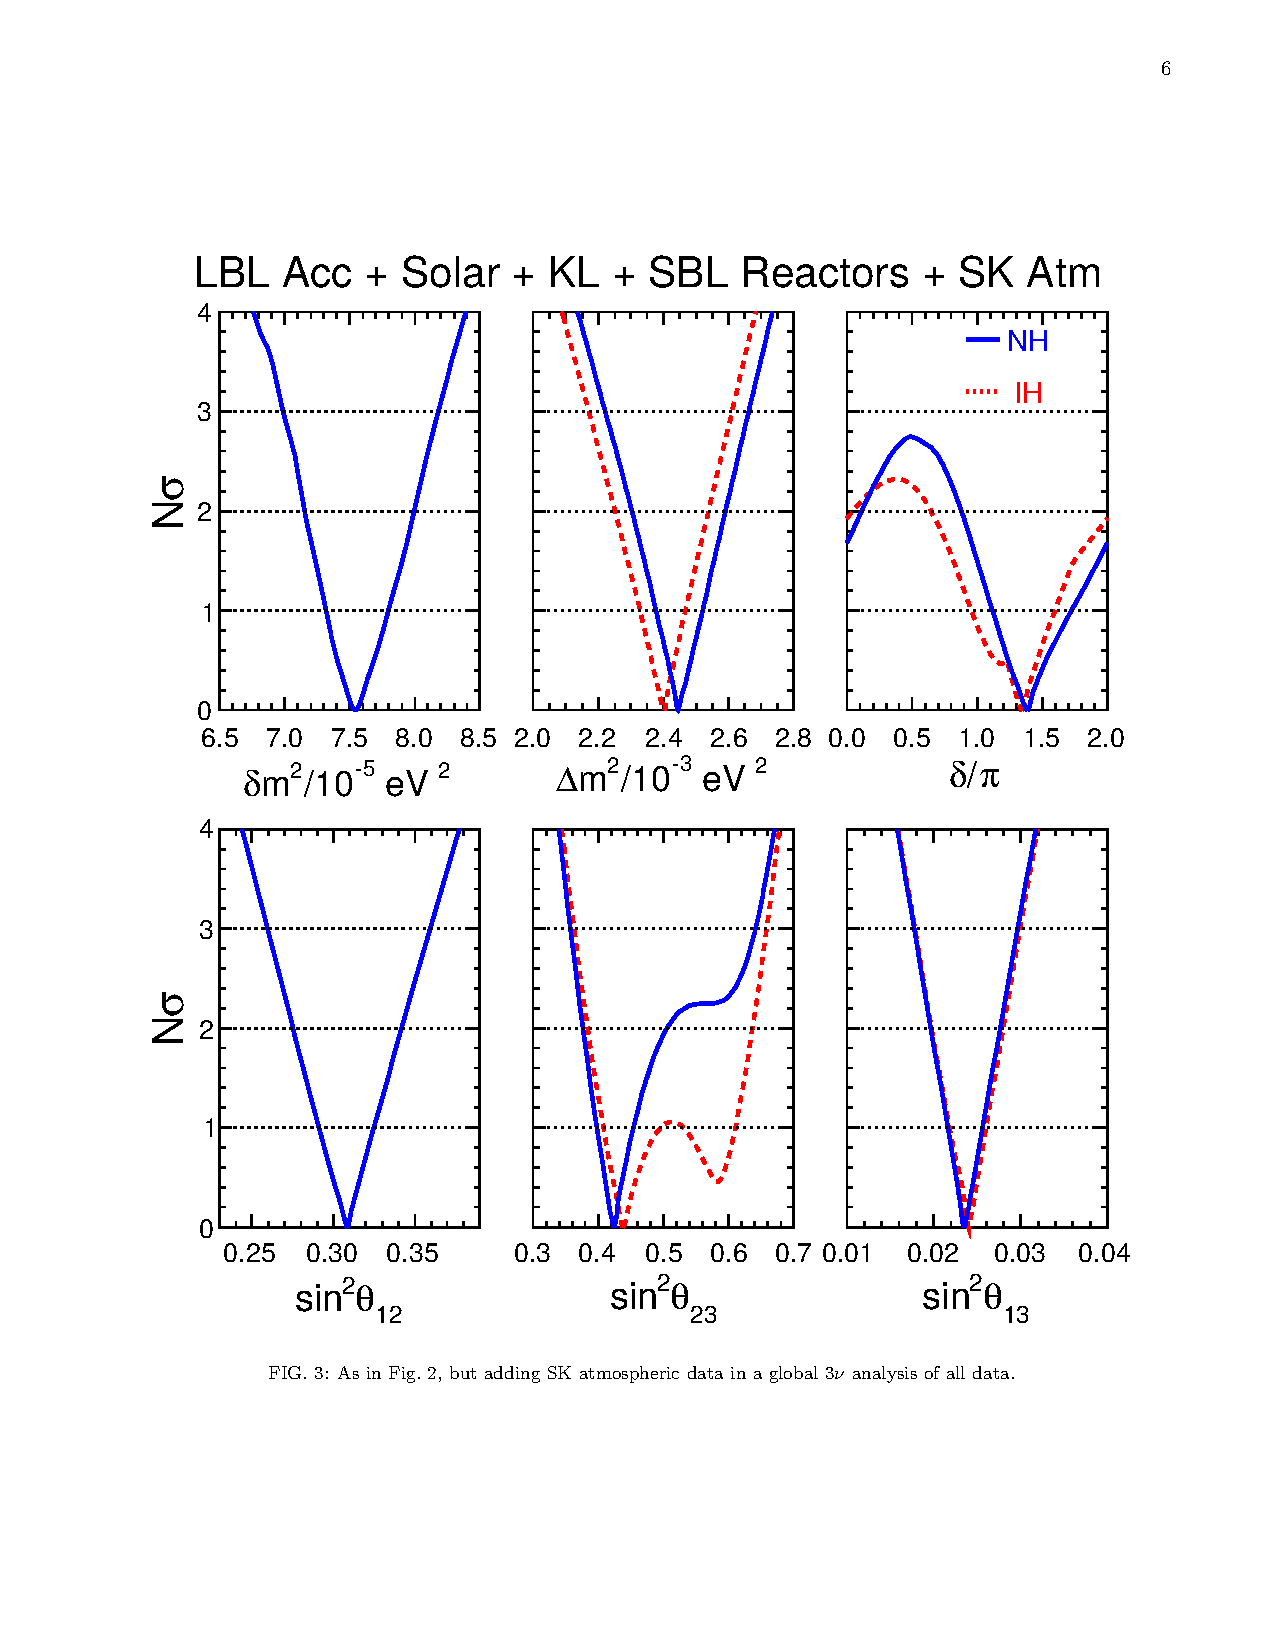
\includegraphics[width=0.8\textwidth,clip,trim=2cm 50mm 2cm 4cm]{figs/fogli13_chisq.pdf}
  \caption[Measurement of the mixing parameters from Capozzi
  {\em et al.}]{Results of the 2013 global analysis from Capozzi {\em et al.} shown as
  N$\sigma$ bounds on the six parameters governing three $\nu$ flavor 
  oscillations. Blue (solid)
    and red (dashed) curves refer to NH and IH, respectively. 
    Figure is from \cite{Capozzi:2013csa}.}
  \label{fig:fogli2013pdfs}
\end{figure}
%


\section{Calculation of Experimental Sensitivities using GLoBES}
\label{sect:globes}
The sensitivity of LBNE to the mass hierarchy, CP violation, and the
octant of $\thetatwothree$ are calculated using the 
GLoBES~\cite{Huber:2004ka,Huber:2007ji}
package to simulate the detector
response using ``true'' values of the oscillation parameters based on the global
fit, smearing based on a simple resolution or on a GENIE\cite{Andreopoulos:2009zz} 
simulation, and detector efficiency values
based on results from ICARUS\cite{icarus-url} and earlier simulation efforts.  
The oscillation parameters used in GLoBES are shown in Table~\ref{tab:oscpar_inputs}.
The detector efficiencies and the energy resolution for $\nu_e$ charged current (CC) 
and $\nu_{\mu}$ CC interactions used in GLoBES are shown in 
Table~\ref{tab:lar-nuosc-totaltable}.
The smearing matrices for $\nu_{\mu}$ neutral current (NC) and $\nu_{\tau}$
interactions are shown in Fig.~\ref{fig:smear_inputs}.
%
\begin{table}[!htb]
\caption{Oscillation parameter inputs used in GLoBES sensitivity calculations.
Central values are taken from the global fit in \cite{Capozzi:2013csa}. 
Angles are in radians.
Relative uncertainty is defined using 1/6 of the full 3$\sigma$ range 
from \cite{Capozzi:2013csa}. In the case of $\theta_{13}$, the relative uncertainty
is based on the current systematic uncertainty in $\sin^22\theta_{13}$ 
from Daya Bay~\cite{An:2013zwz} as an approximation of the ultimate precision of the 
current generation of reactor experiments.}
\begin{center}
\begin{tabular}{l|c|c|c}
\hline\hline
Parameter & Hierarchy & Central Value & Relative Uncertainty \\ \hline \hline
$\Delta m^2_{21}$/10$^{-5}$ eV$^2$ & NH/IH & 7.54 & 3\% \\ \hline
$\theta_{12}$                      & NH/IH & 0.588 & 3\% \\ \hline
$\Delta m^2_{31}$/10$^{-3}$ eV$^2$ & NH    & 2.48 & 3\% \\
                                   & IH    & -2.36 & 3\% \\ \hline
$\theta_{13}$                      & NH    & 0.154 & 3\% \\
                                   & IH    & 0.155 & 3\% \\ \hline
$\theta_{23}$                      & NH    & 0.710 & 7\% \\
                                   & IH    & 0.722 & 7\% \\ \hline
$\delta_{CP}$                      & NH/IH & scan  & no constraint \\ \hline
\end{tabular}
\end{center}
\label{tab:oscpar_inputs}
\end{table}
%
\begin{table}[!htb]
\caption{Signal and background effienciencies, normalization uncertainties, and
  energy resolutions, 
  which are obtained from ICARUS and earlier simulation efforts, used in the GLoBES 
  sensitivity calculations.}
\label{tab:lar-nuosc-totaltable}
\begin{center}
\begin{tabular}{l|c}
\hline \hline
Parameter & Value Used for  LBNE Sensitivities\\  \hline\hline
& For $\nu_e$-CC appearance \\ \hline
$\nu_e$-CC efficiency          & 80\%   \\ 
$\nu_\mu$-NC mis-identification rate  & 1\%   \\ 
$\nu_\mu$-CC mis-identification rate  & 1\%   \\ 
Other background                 & 0\% \\ 
Signal normalization error       & 1\% \\ 
Background normalization error   & 5\% \\  \hline
& For $\nu_\mu$-CC disappearance \\ \hline
$\nu_\mu$-CC efficiency          & 85\%   \\ 
$\nu_\mu$-NC mis-identification rate  & 1\%   \\ 
Other background                 & 0\% \\ 
Signal normalization error       & 5\% \\ 
Background normalization error   & 10\% \\ \hline
& Neutrino Energy Resolutions \\ \hline
$\nu_e$ CC energy resolution & $15\%/\sqrt{E(GeV)}$ \\
$\nu_{\mu}$ CC energy resolution & $15\%/\sqrt{E(GeV)}$ \\ \hline
\end{tabular}
\end{center} 
\end{table}
%
\begin{figure}[!htb]
  \centering
  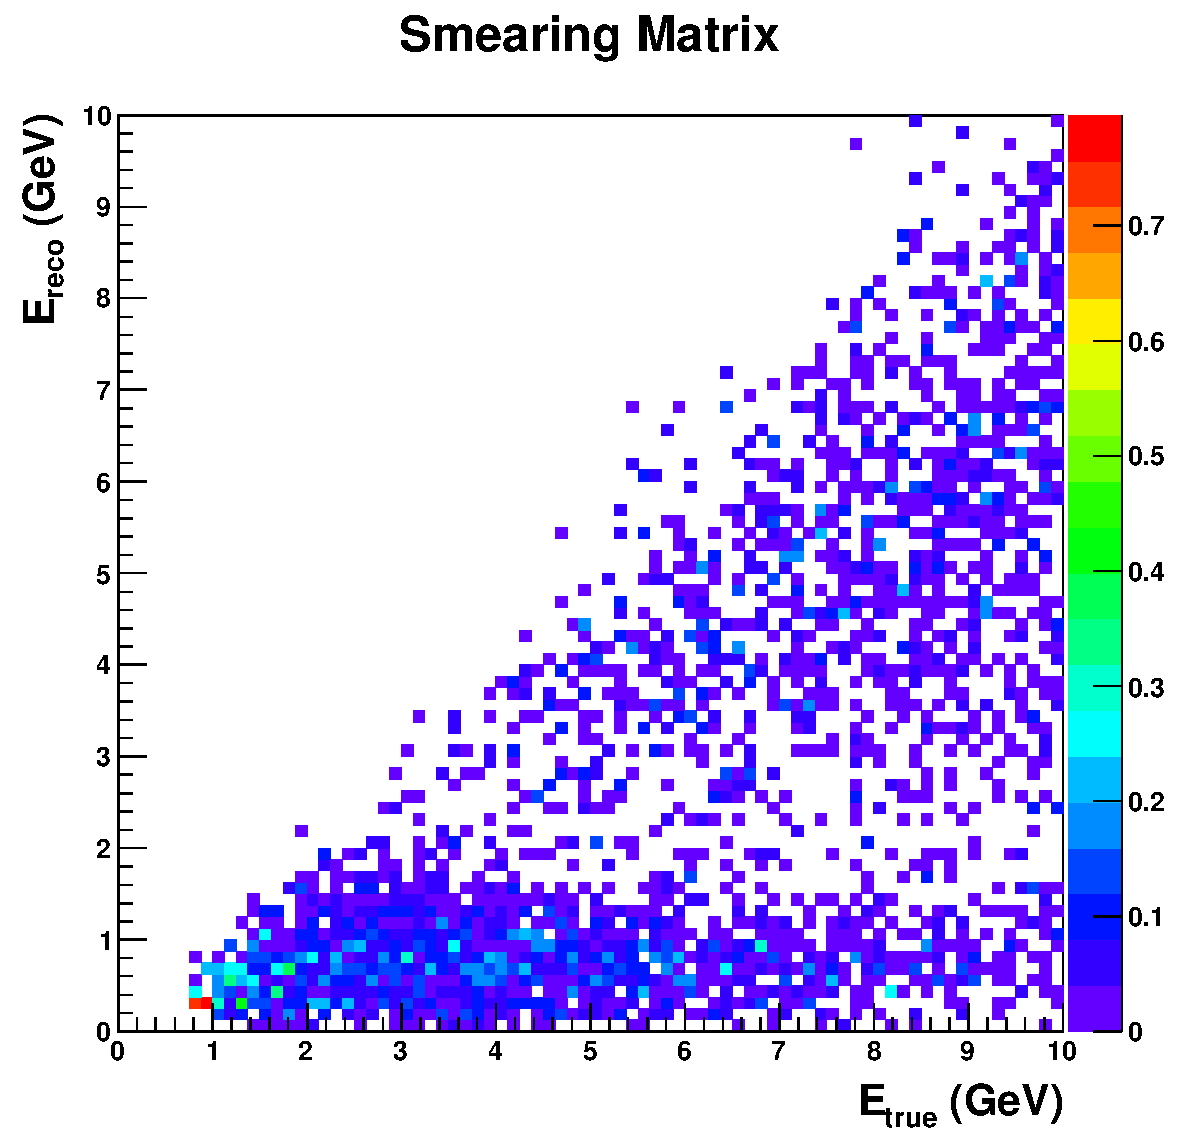
\includegraphics[width=0.45\textwidth]{figs/LBNE_smear_NC_all.pdf}
  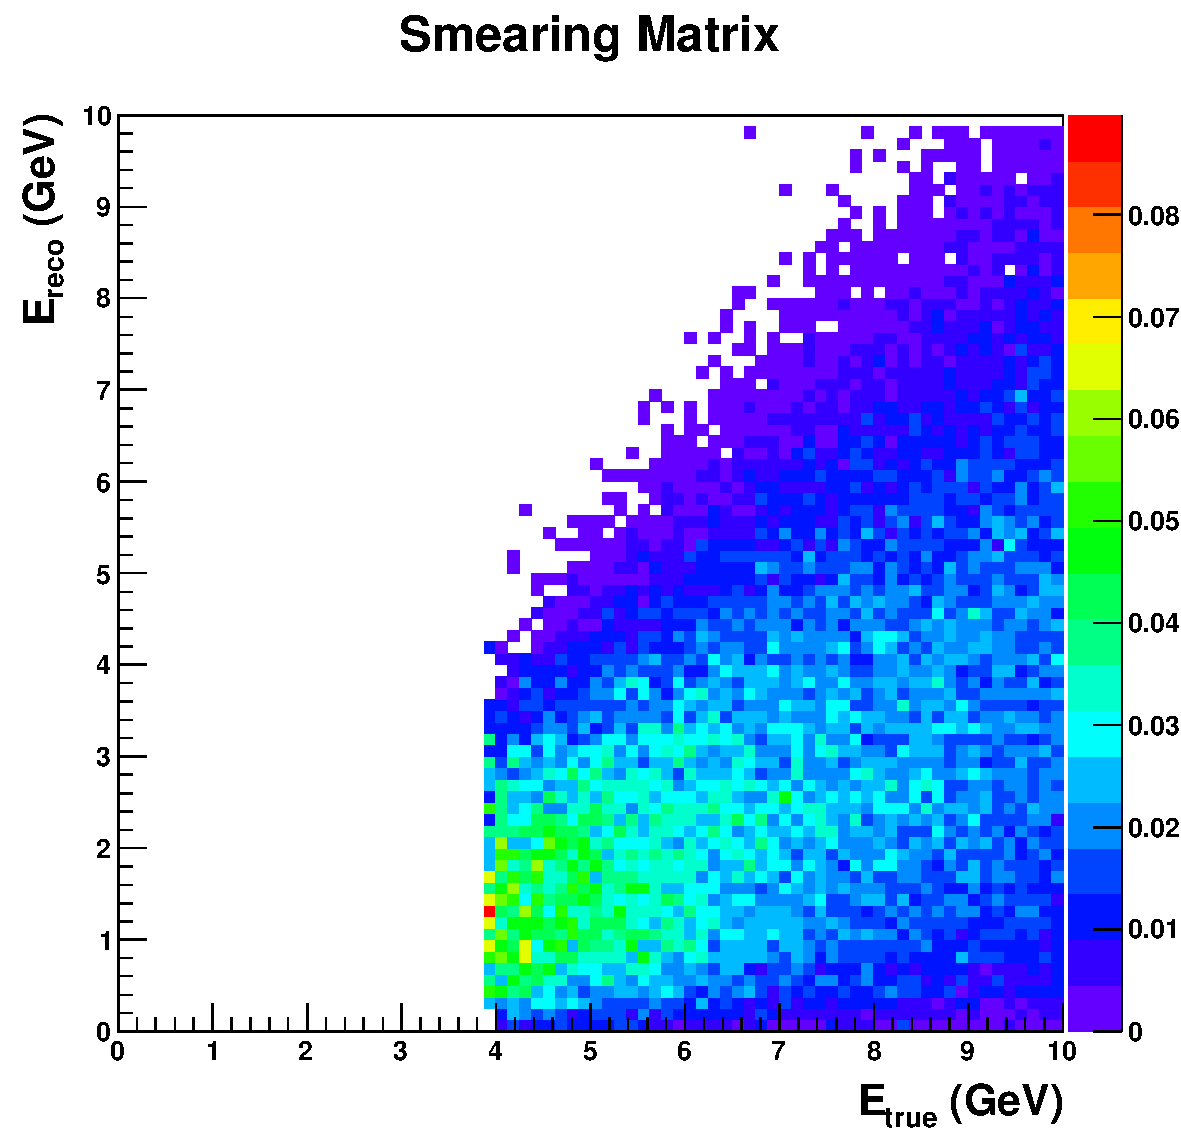
\includegraphics[width=0.45\textwidth]{figs/tau_smear_prd.pdf}
  \caption{$\nu_{\mu}$ NC (left) and $\nu_{\tau}$ energy smearing matrices, produced
  using a GENIE simulation, used in the GLoBES senstivitiy calculations.}
  \label{fig:smear_inputs}
\end{figure}

Estimates of experimental sensitivity are obtained in GLoBES
by simultaneously fitting the $\nu_\mu \rightarrow \nu_\mu$,
$\overline{\nu}_\mu \rightarrow \overline{\nu}_\mu$, $\nu_\mu \rightarrow \nu_e$, 
and  $\overline{\nu}_\mu \rightarrow \overline{\nu}_e$ oscillated spectra, examples of
which are shown in Figure~\ref{fig:example_spectra}.
In these calculations, experimental sensitivity is
quantified using $\Delta\chi^2$ parameters, which are determined
by comparing the predicted spectra for various scenarios. 
These quantities are defined, differently for neutrino MH, CP-violation, and octant 
sensitivity, to be:
\begin{eqnarray}
\Delta\chi^2_{MH} & = & |\chi^2_{MH^{test}=IH} - \chi^2_{MH^{test}=NH}|, \\
\Delta\chi^2_{CPV} & = & \min\left(\Delta\chi^2_{CP}(\delta_{CP}^{test}=0),\Delta\chi^2_{CP}(\delta_{CP}^{test}=\pi)\right)\mbox{, where} \\
\Delta\chi^2_{CP} & = & \chi^2_{\delta_{cp}^{test}} - \chi^2_{\delta_{CP}^{true}}\mbox{, and} \\
\Delta\chi^2_{octant} & = & |\chi^2_{\theta_{23}^{test}>45^\circ} - \chi^2_{\theta_{23}^{test}<45^\circ}|. \\ \nonumber
\end{eqnarray}
These sensitivities are evaluated separately for true NH and IH. 
Since the true value of $\delta_{CP}$ is unknown, a scan is  performed over
all possible values of $\delta_{CP}^{true}$. For the case of the octant sensitivity,
the value of $\theta_{23}$ in the ``wrong'' octant is constrained only to have a value 
within the ``wrong'' octant, i.e., it is not required to have the same value of 
$\sin^22\theta_{23}$ as the true value.
The individual $\chi^2$ values are calculated using
\begin{equation}
\chi^2({\bf n}^{true},{\bf n}^{test},f) = 2 \sum_{i}^{N_{reco}} (n_i^{true} ln\frac{n_i^{true}}{n_i^{test}(f)} + n_i^{test}(f) - n_i^{true}) + f^2,
\label{eq:globes_chisq}
\end{equation}
where {\bf n} are event rate vectors in $N_{reco}$ bins of reconstructed energy and $f$ represents
a nuisance parameter 
to be profiled. Nuisance parameters include the values of mixing angles, 
mass splittings, and signal and
background normalization. The nuisance parameters are constrained by Gaussian priors; 
in the
case of the oscillation parameters, the Gaussian prior has standard deviation
determined by taking 1/6 of the 3$\sigma$ range allowed by the global 
fit~\cite{Fogli:2012ua}. 
\begin{figure}[!htb]
  \centering
  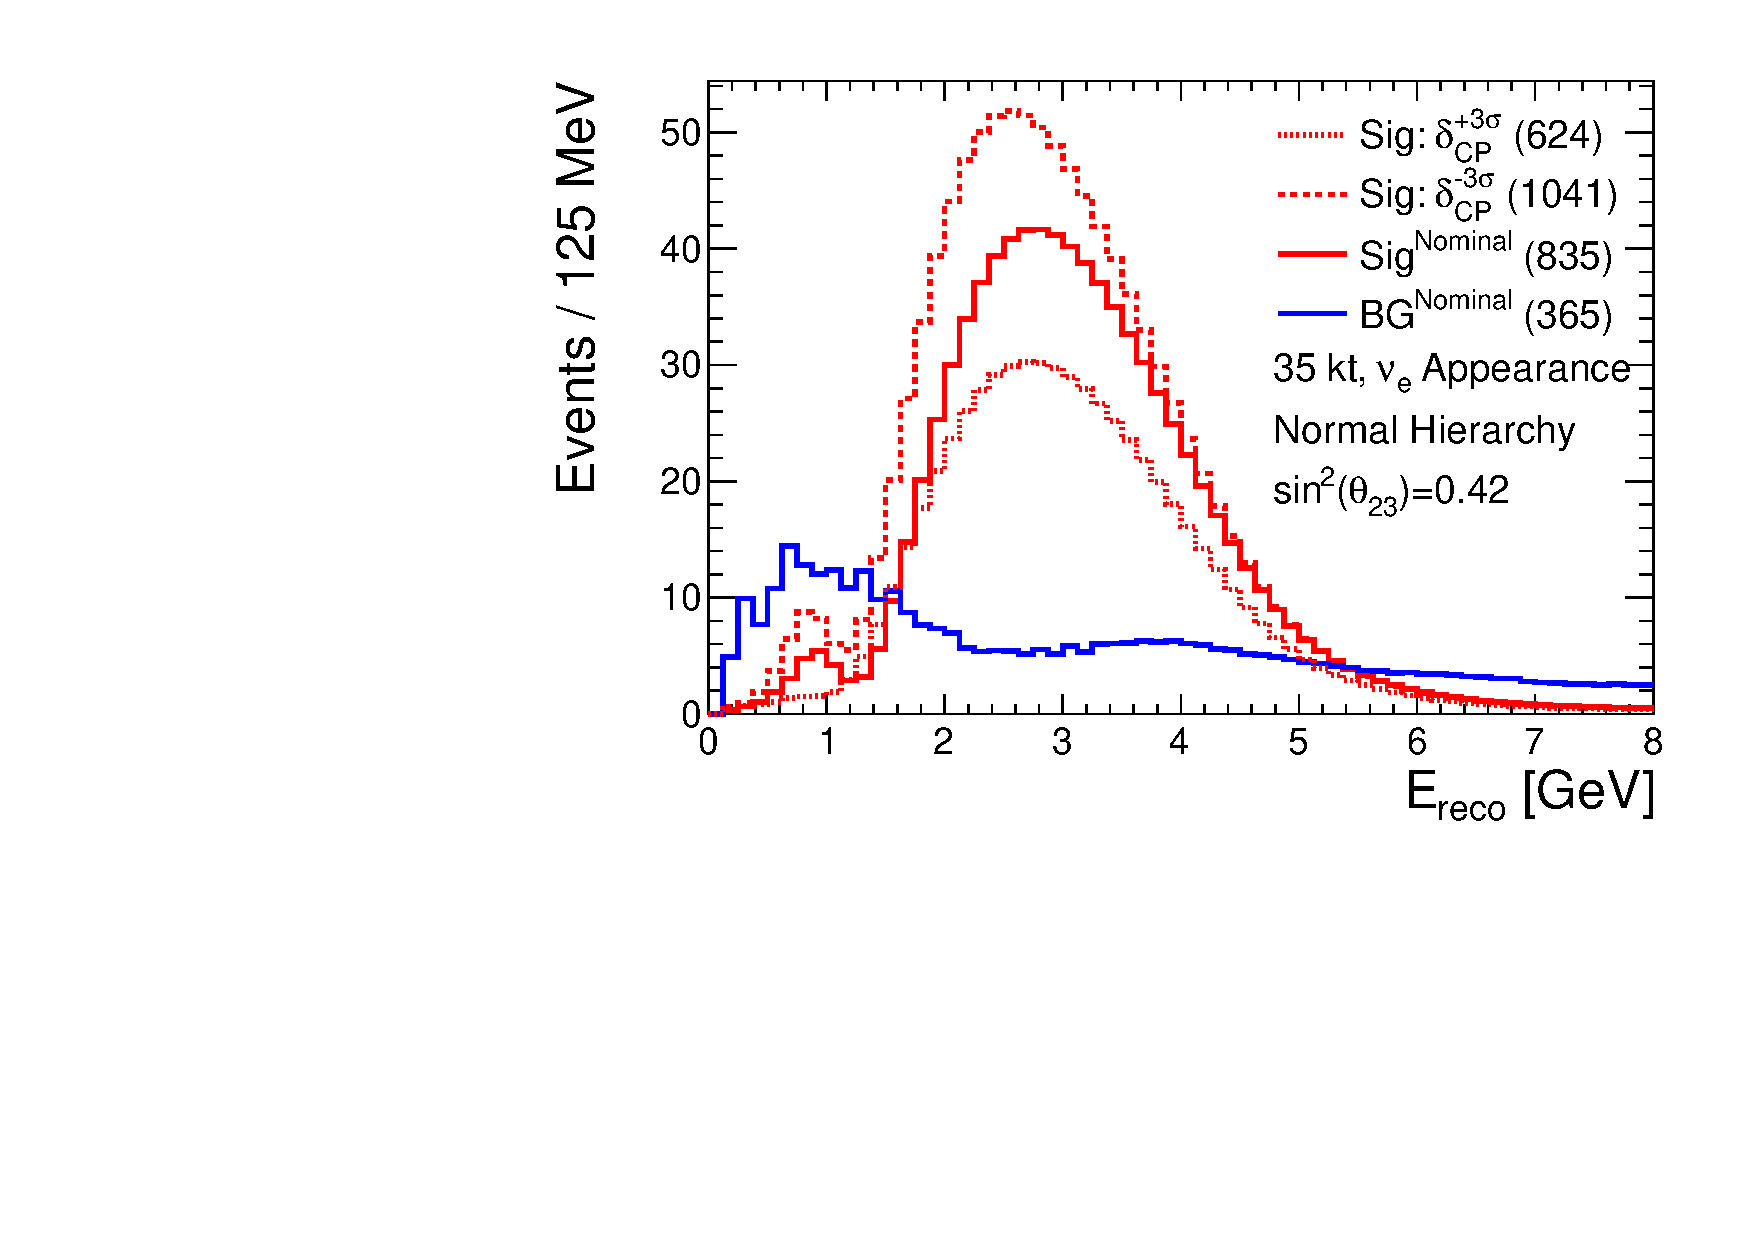
\includegraphics[width=0.45\textwidth]{figs/spectra_35kt_nue_dcpvar_nh.pdf}
  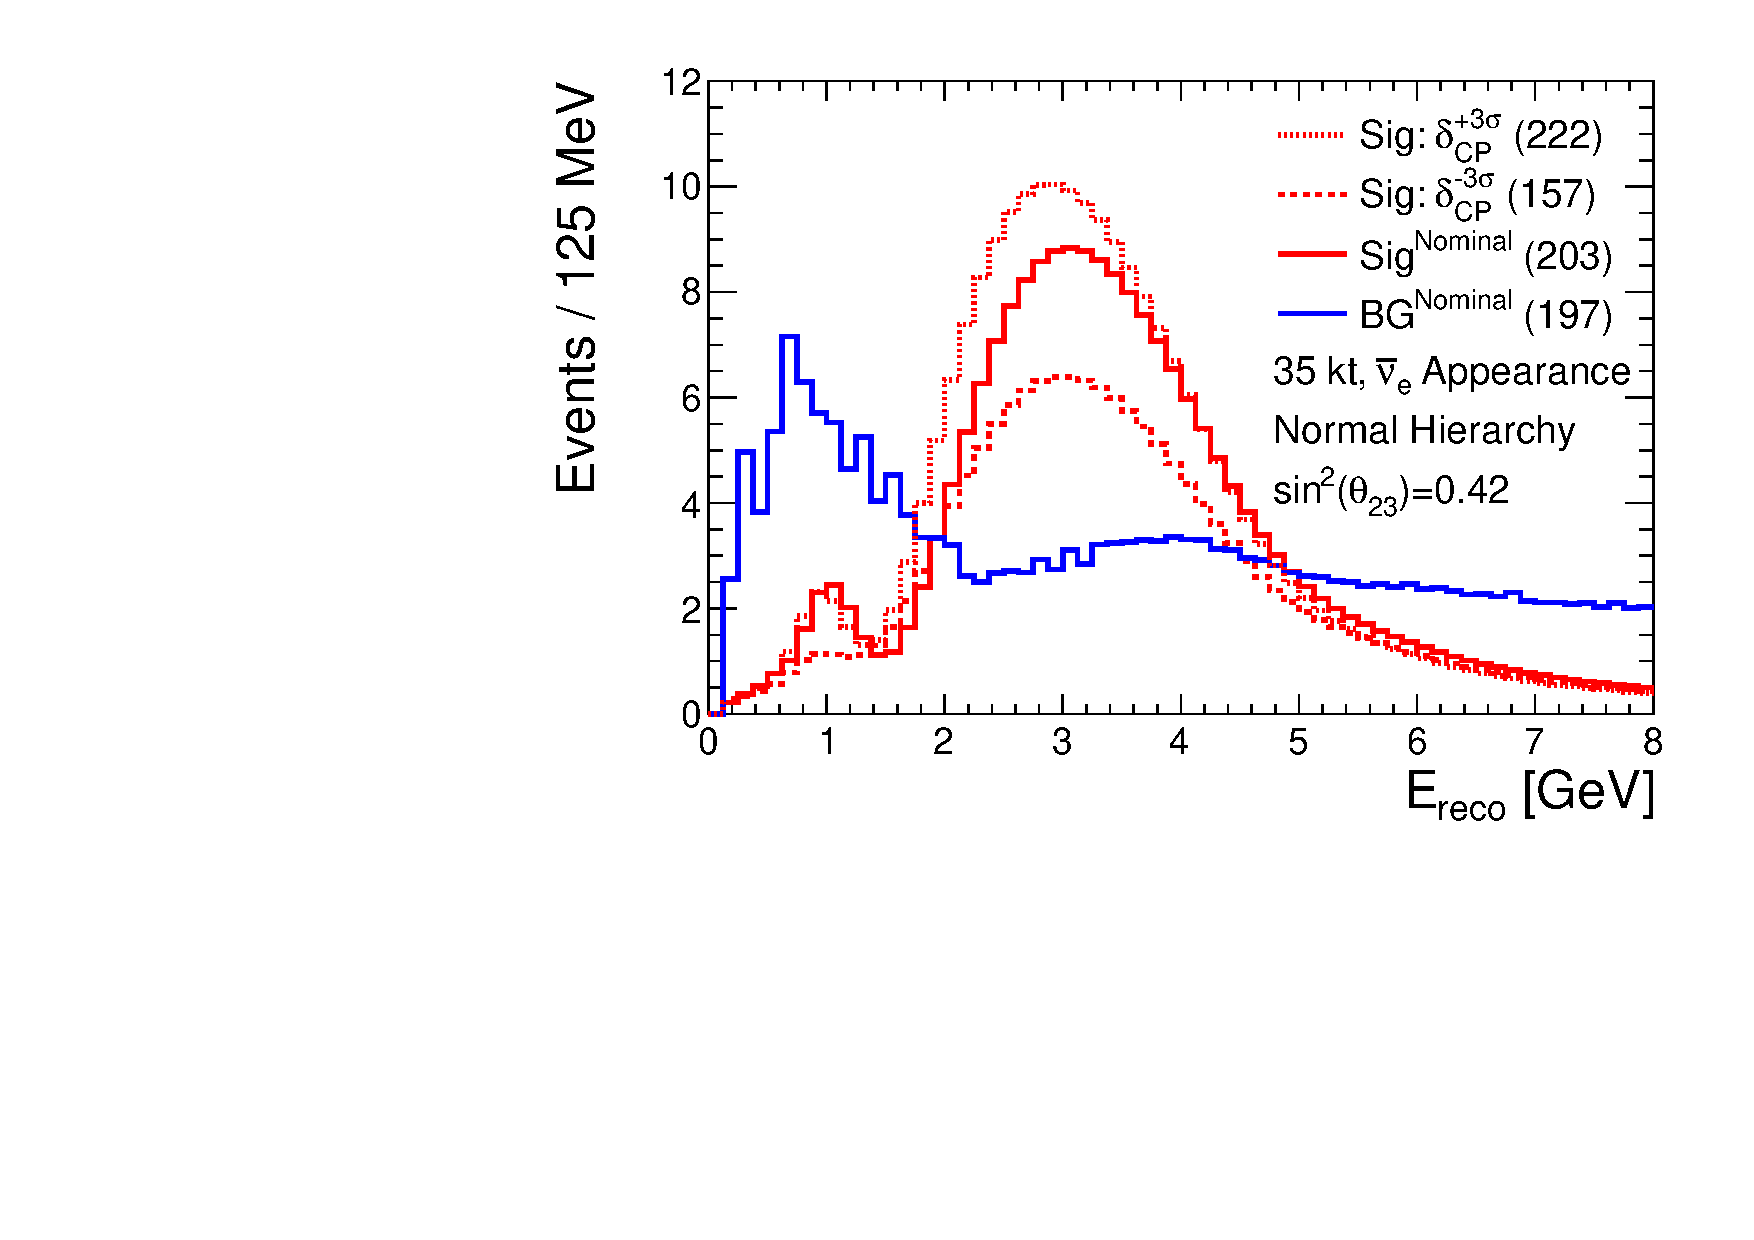
\includegraphics[width=0.45\textwidth]{figs/spectra_35kt_nuebar_dcpvar_nh.pdf}
  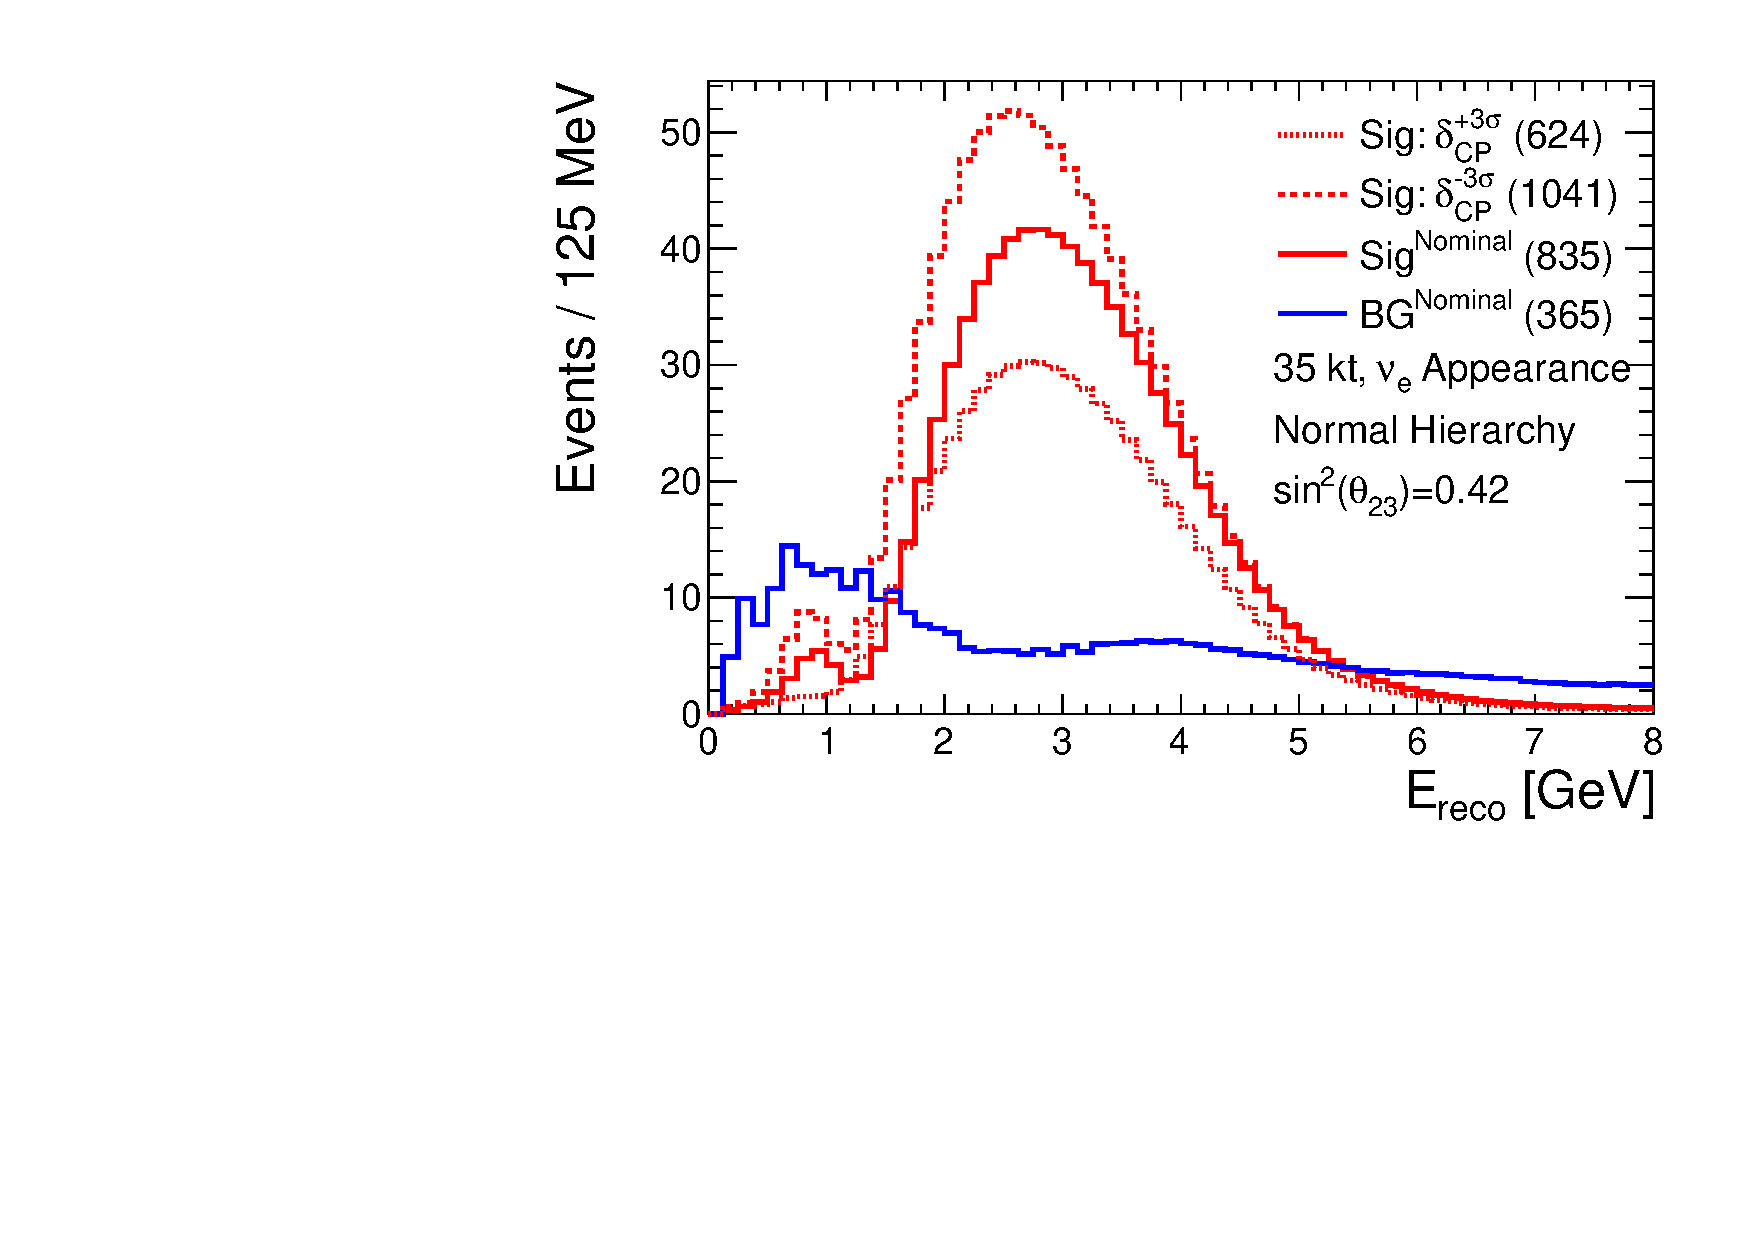
\includegraphics[width=0.45\textwidth]{figs/spectra_35kt_nue_dcpvar_nh.pdf}
  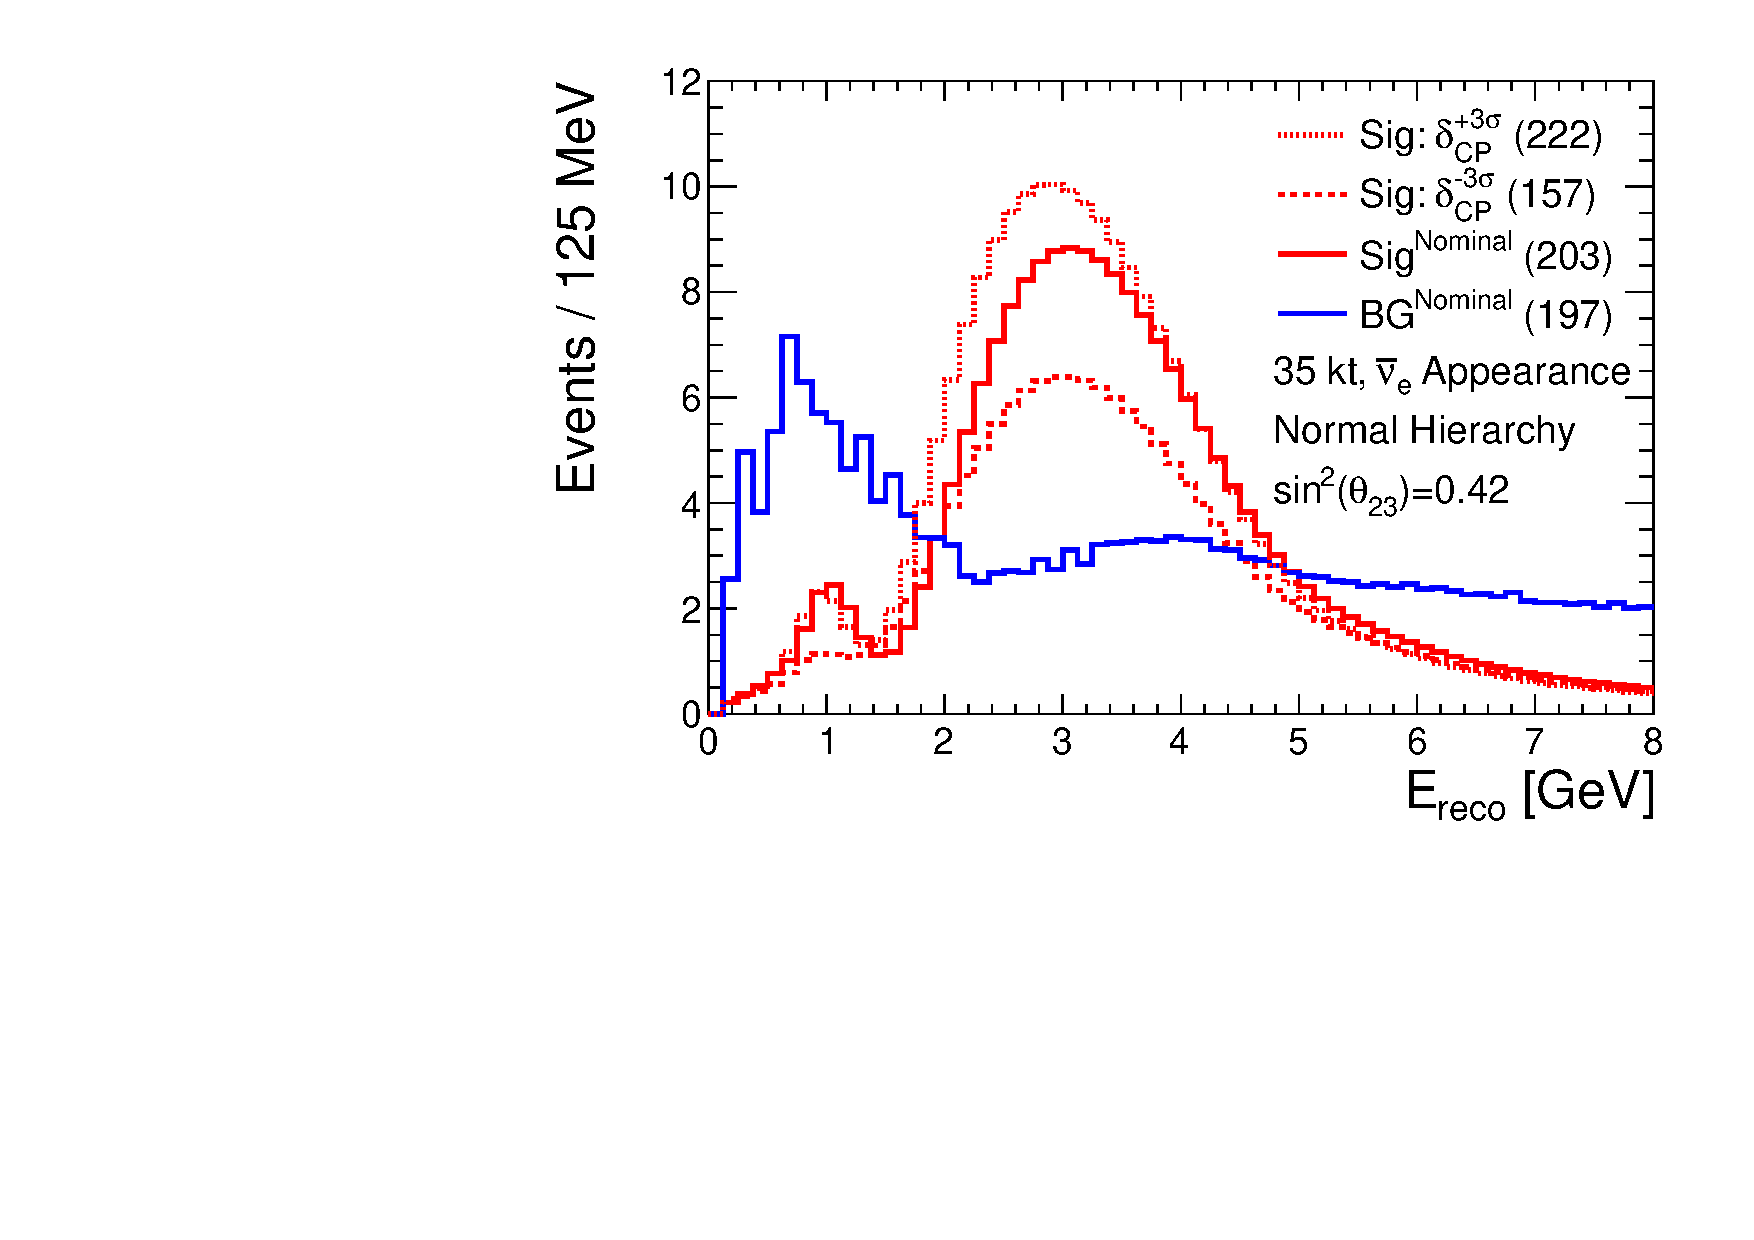
\includegraphics[width=0.45\textwidth]{figs/spectra_35kt_nuebar_dcpvar_nh.pdf}
  \caption{FIXME: Get real disappearance plots.
  Examples of spectra produced by GLoBES for a 35-kt LArTPC with 3 years of 
  exposure in an 80-GeV, 1.2-MW beam, for the case of true NH. 
  $\nu_{\mu}$~disappearance (top left),
  $\overline{\nu}_{\mu}$~disappearance (top right), $\nu_e$~appearance (bottom left),
  and $\overline{\nu}_e$~appearance (bottom right). The effect of varying the true
  value of $\delta_{CP}$ from -$\pi/2$ to zero to $\pi/2$ is shown. The total background,
  which does not depend on $\delta_{CP}$, is overlaid on the signal. The total number
  of signal and background events are indicated in parenthesis.}
  \label{fig:example_spectra}
\end{figure}

LBNE's sensitivity to MH and CPV is based on observation of the neutrino-antineutrino 
asymmetry,
\begin{equation}
A_{CP} = \frac{P(\nu_\mu \rightarrow \nu_e) -
  P(\overline{\nu}_\mu \rightarrow \overline{\nu}_e)}{P(\nu_\mu \rightarrow
  \nu_e) + P(\overline{\nu}_\mu \rightarrow \overline{\nu}_e)}.
\end{equation}
This asymmetry contains contributions both from 
the different effective masses of neutrinos and antineutrinos as they propagate 
in matter and from CP violation related to $\delta_{CP}$.
Figure~\ref{fig:cpasymm} shows the total asymmetry at 1300 km for the first
and second oscillation nodes, for both NH and IH.
There is a nearly degenerate value for the asymmetries at $\delta_{CP}\sim\pi/2$, 
true NH and at $\delta_{CP}\sim-\pi/2$, true IH in the first oscillation node. This
is the reason for the decrease in MH sensitivity for long-baseline experiments in
the region near $\delta_{CP}\sim\pi/2$. Shorter baseline experiments also see
degradation of CPV sensitivity in this region \cite{NOVA/T2K}, but in LBNE, the MH
will be resolved with sufficient precision that the CPV sensitivity is not strongly
affected by degeneracies. Fig.~\ref{fig:cpasymm} also highlights the critical importance
of experimental access to the second oscillation node, where the CP asymmetry is larger,
so no such degeneracy with the matter effect is present. 
%
\begin{figure}[!htb]
  \centering
  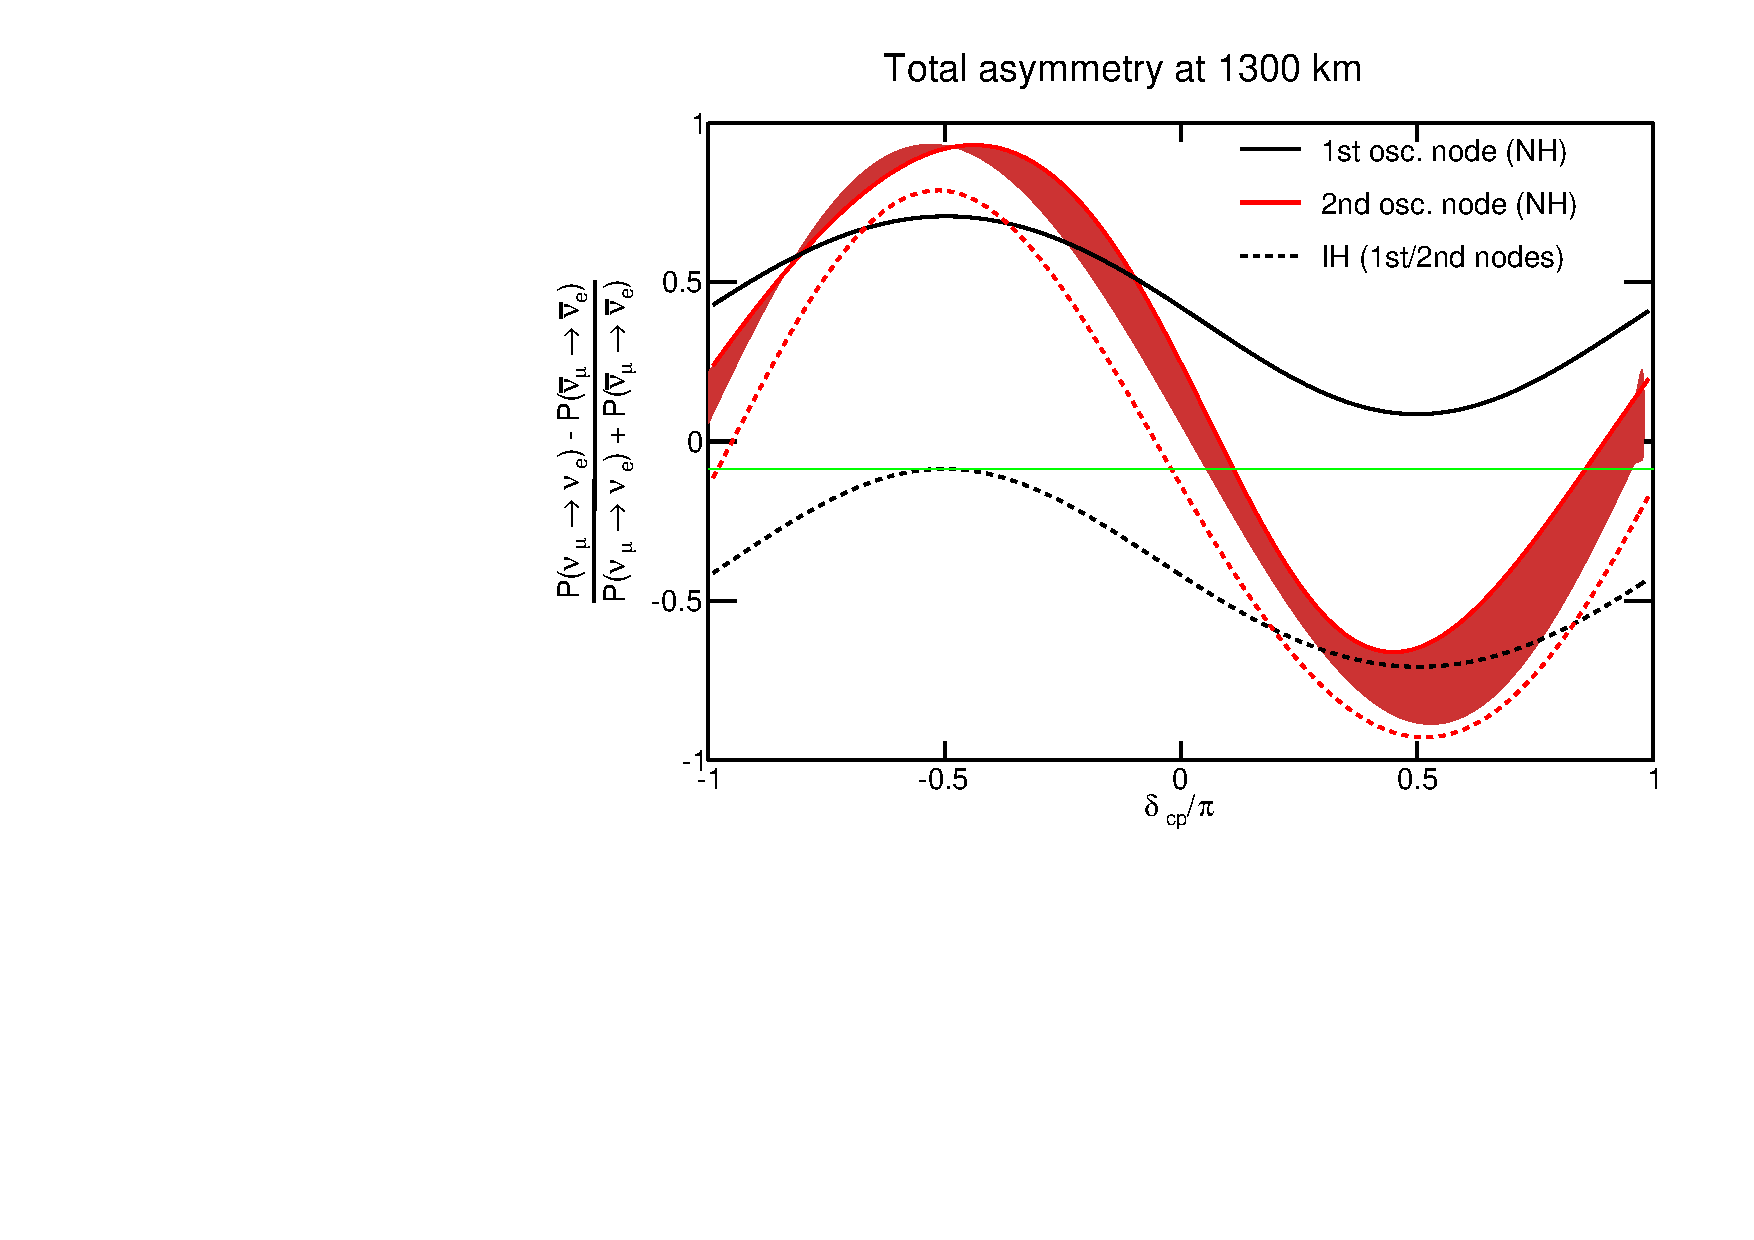
\includegraphics[width=0.75\textwidth]{figs/asym_vs_dcp_1300km.pdf}
  \caption{Neutrino-antineutrino asymmetry as a function of $\delta_{CP}$ for
  the first (black) and second (red) oscillation nodes, for NH (solid) and IH (dashed),
  at the LBNE baseline of 1300 km.} 
  \label{fig:cpasymm}
\end{figure}

\section{Sensitivity Dependence on $\thetaonethree$}
\label{sect:t13}

Figure \ref{fig:th13spec} shows the variation in $\nu_e$ and $\overline{\nu}_e$
appearance signal when the true value of $\theta_{13}$ is varied within its 3$\sigma$
allowed range. 
\begin{figure}[!htb]
  \centering
  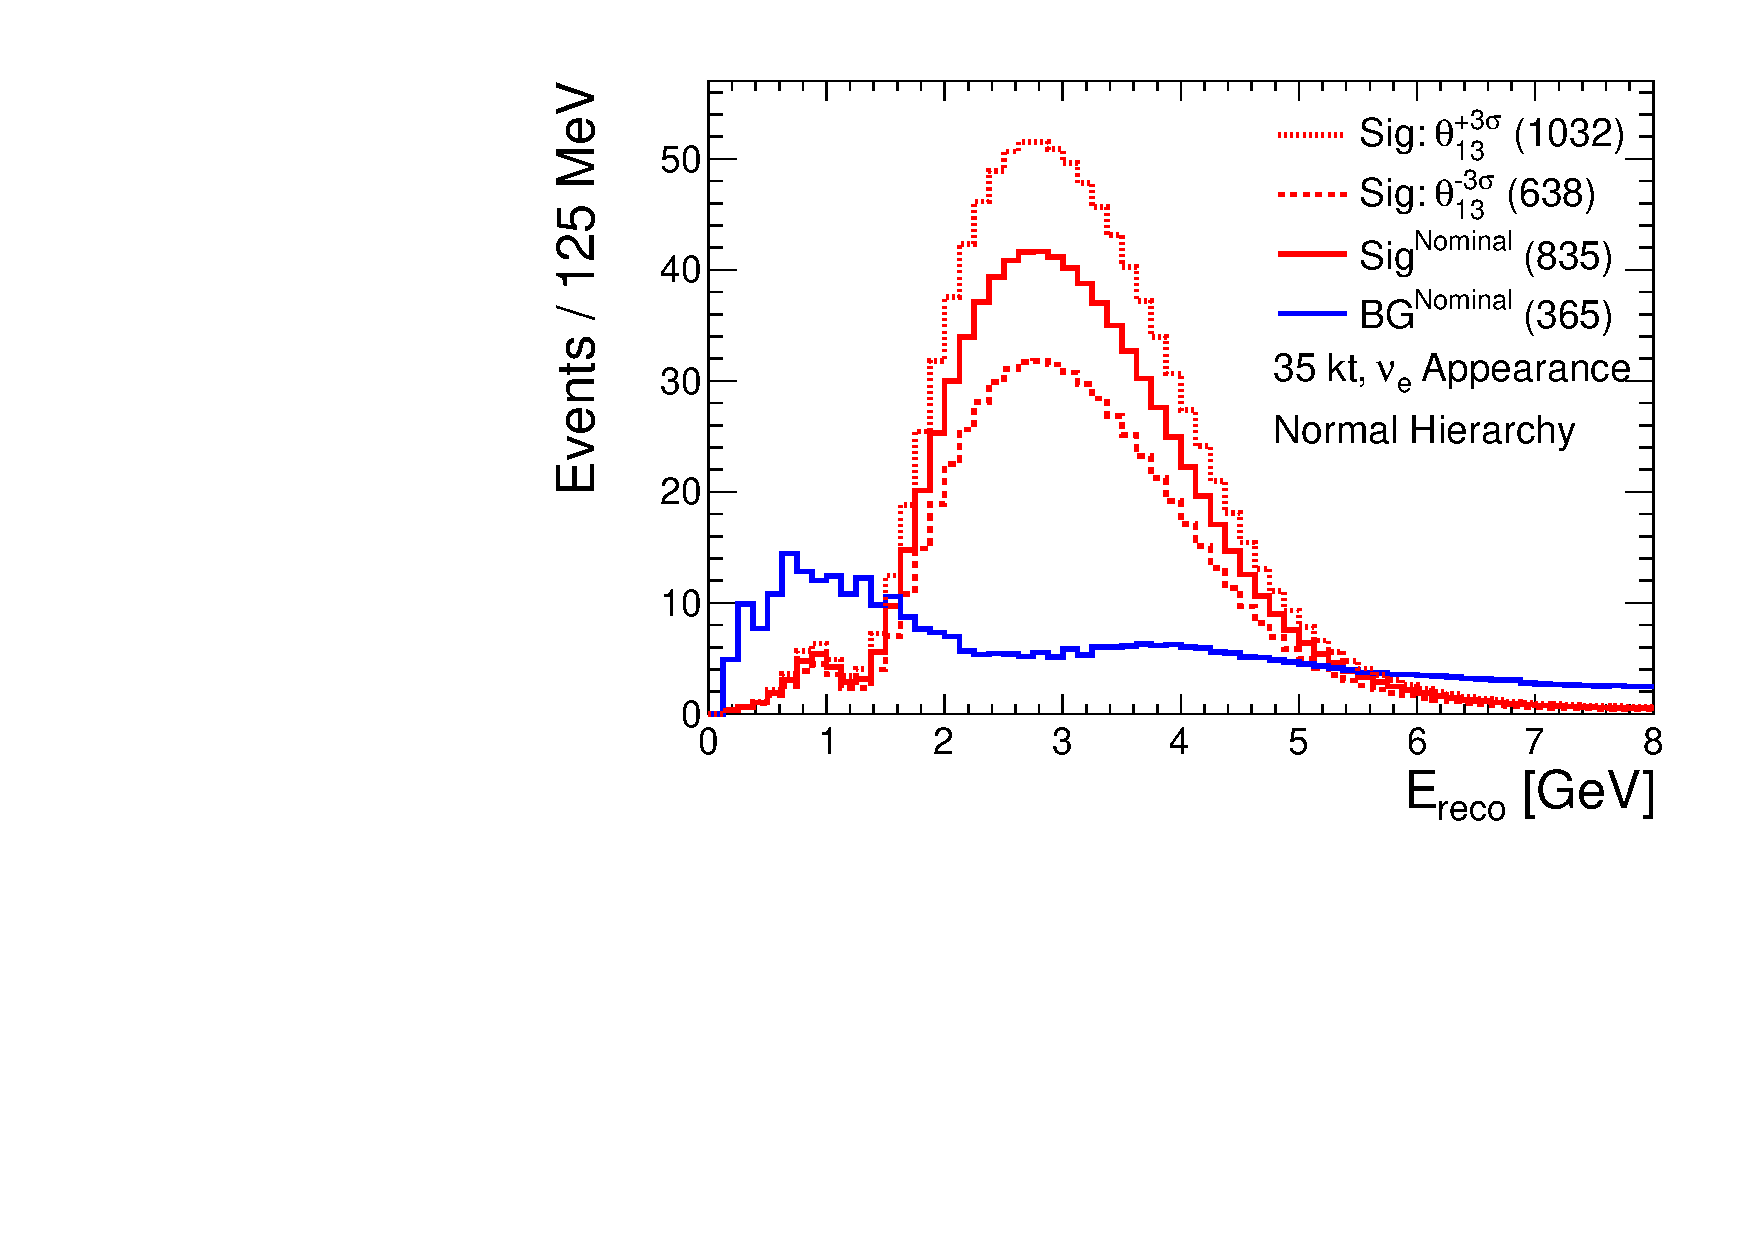
\includegraphics[width=0.45\textwidth]{figs/spectra_35kt_nue_th13var_nh.pdf}
  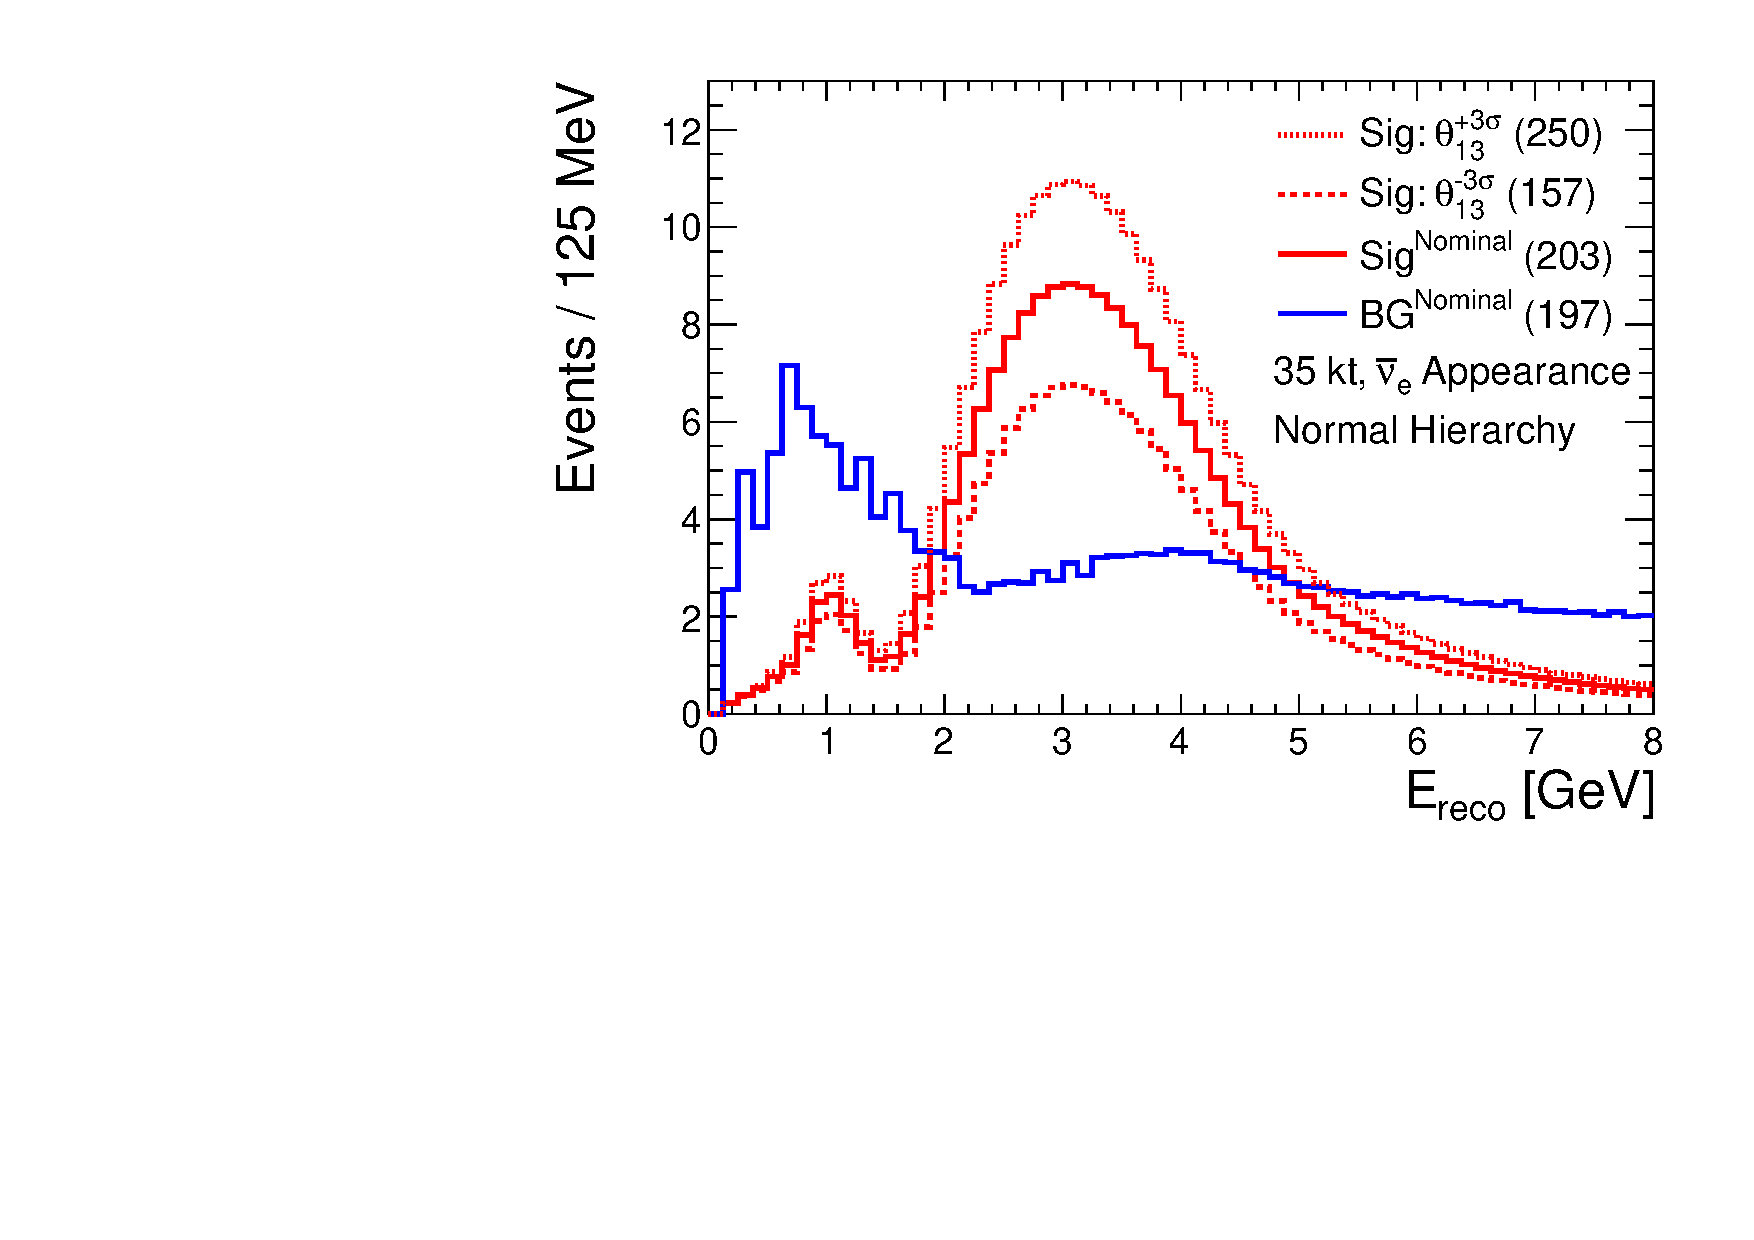
\includegraphics[width=0.45\textwidth]{figs/spectra_35kt_nuebar_th13var_nh.pdf}
  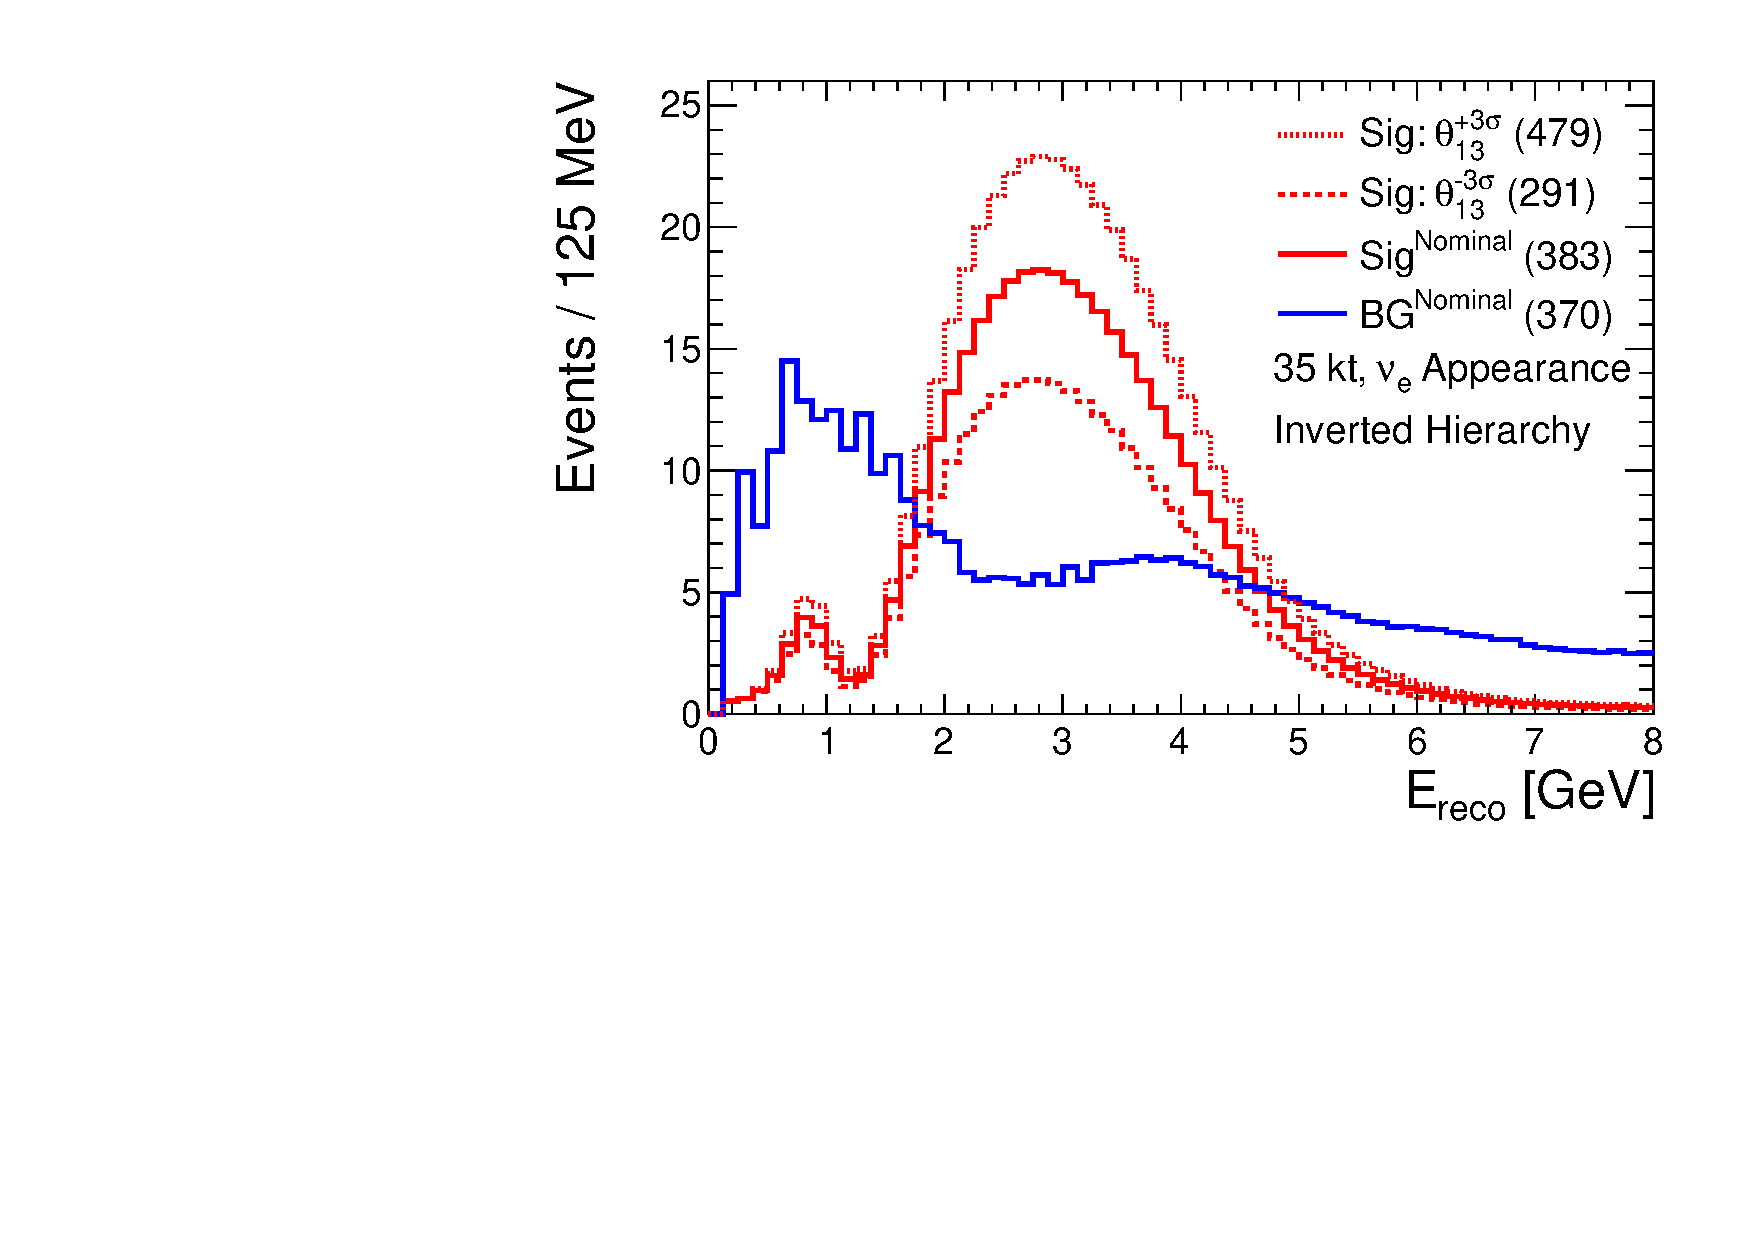
\includegraphics[width=0.45\textwidth]{figs/spectra_35kt_nue_th13var_ih.pdf}
  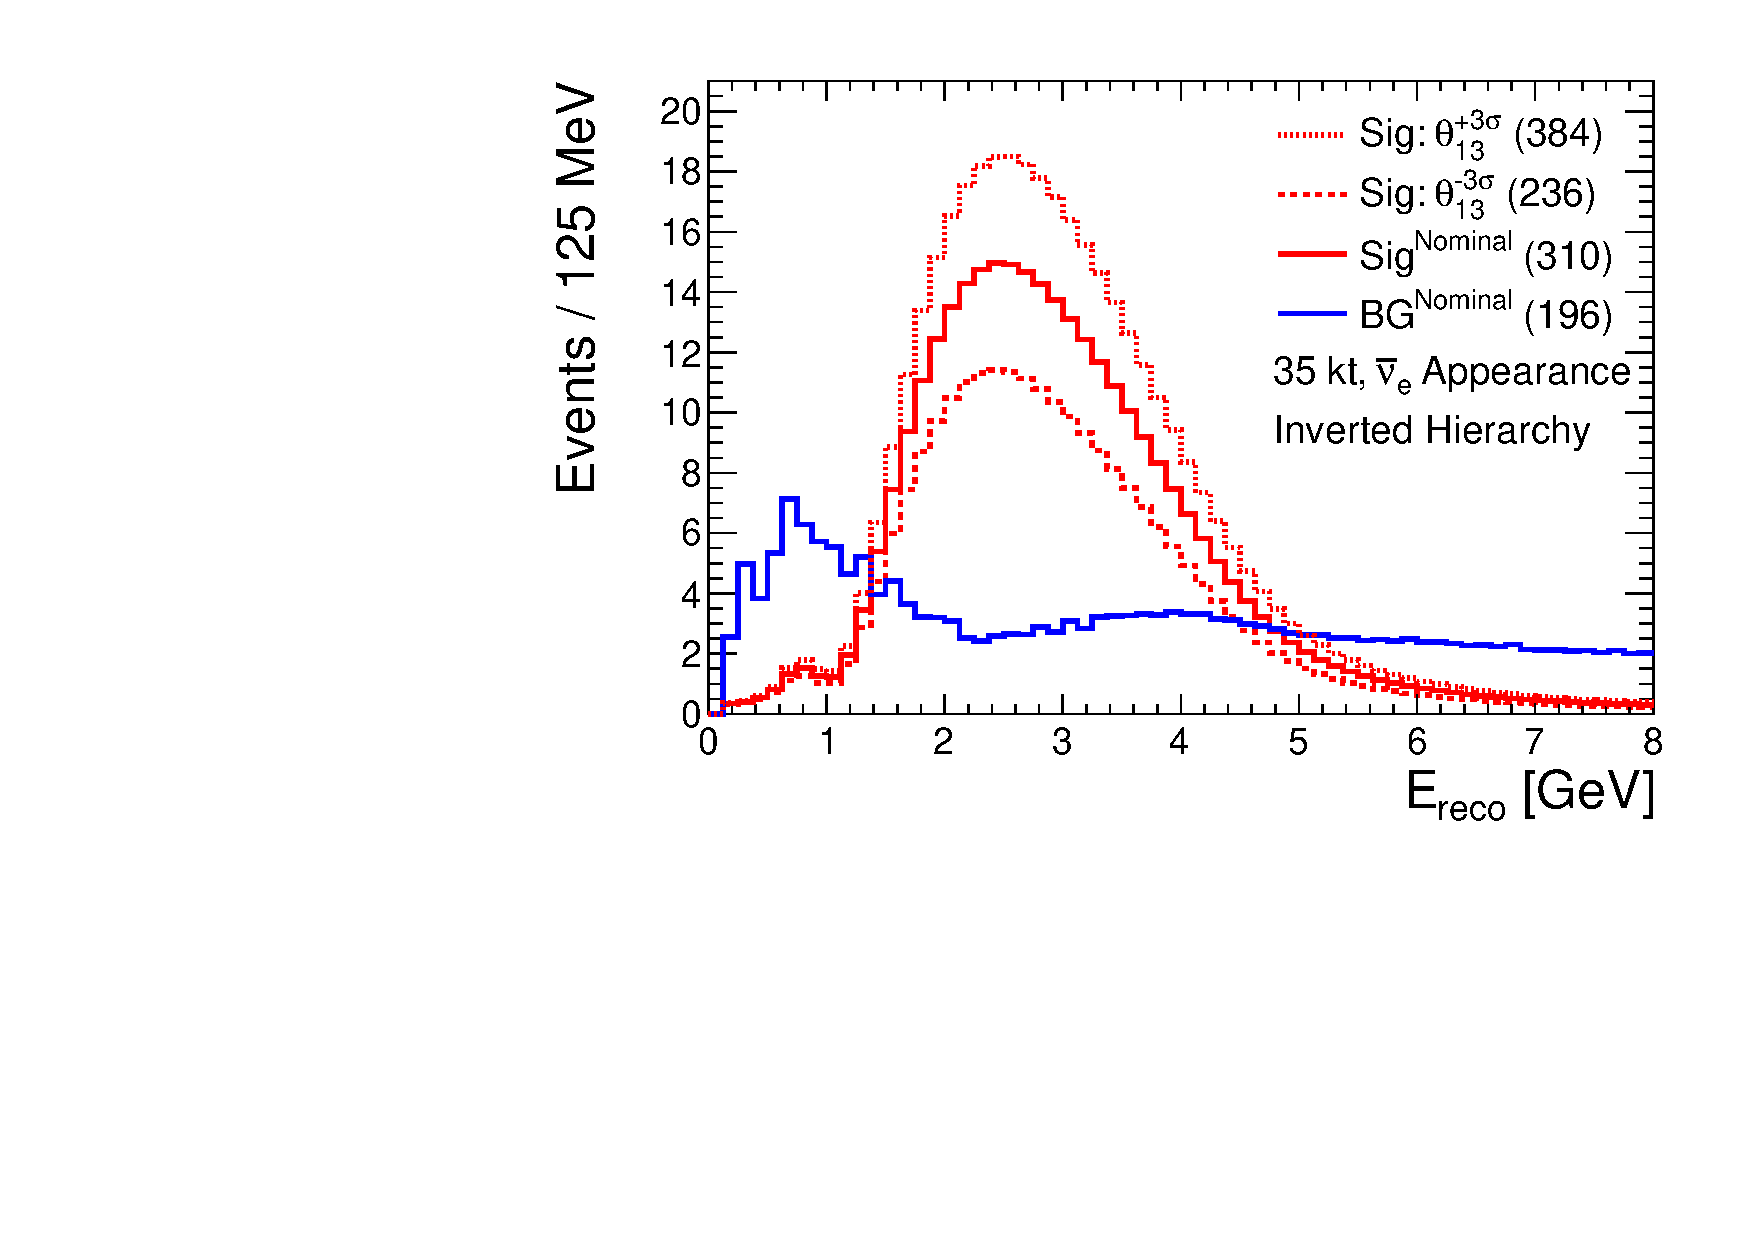
\includegraphics[width=0.45\textwidth]{figs/spectra_35kt_nuebar_th13var_ih.pdf}
  \caption{
  Variations in $\theta_{13}$: 
  $\nu_e$~appearance (left) and $\overline{\nu}_e$~appearance (right) spectra 
  produced by GLoBES for a 35-kt LArTPC with 3 years of 
  exposure in an 80-GeV, 1.2-MW beam,  for true NH (top) and true IH (bottom). 
  The effect of varying the true
  value of $\theta_{13}$ within its 3$\sigma$ allowed range is shown. 
  The total background, which does not depend on value of $\theta_{13}$ (CHECKME), 
  is overlaid on the signal. The total number
  of signal and background events are indicated in parenthesis.}
  \label{fig:th13spec}
\end{figure}
%
The effect of increasing $\theta_{13}$ is an increase in event rate with no change
to the spectral shape. This can be understood by inspection of 
Equation~\ref{eqn:papprox0}, in which $P_0$ includes a factor of $\sin^22\theta_{13}$.
Figure~\ref{fig:th13sens} shows the variation in MH and CPV sensitivity when $\theta_{13}$
is varied within its 1$\sigma$ and 3$\sigma$ allowed range. In each case, the 
nominal relative constraints on all oscillation parameters, including $\theta_{13}$, 
are applied and the normalization constraints are the nominal
1\% for signal and 5\% for background. The increased statistics from increasing
$\theta_{13}$ provides a modest increase in MH sensitivity for both true NH and IH.
The CPV sensitivity does not improve significantly. The slightly larger increase in
sensitivity in IH compared to NH can be understood because the statistics in true IH
are signficantly lower than in true IH, so increasing the sample size has a larger effect.
FIXME: Seems believeable but is this true?
%
\begin{figure}[!htb]
  \centering
  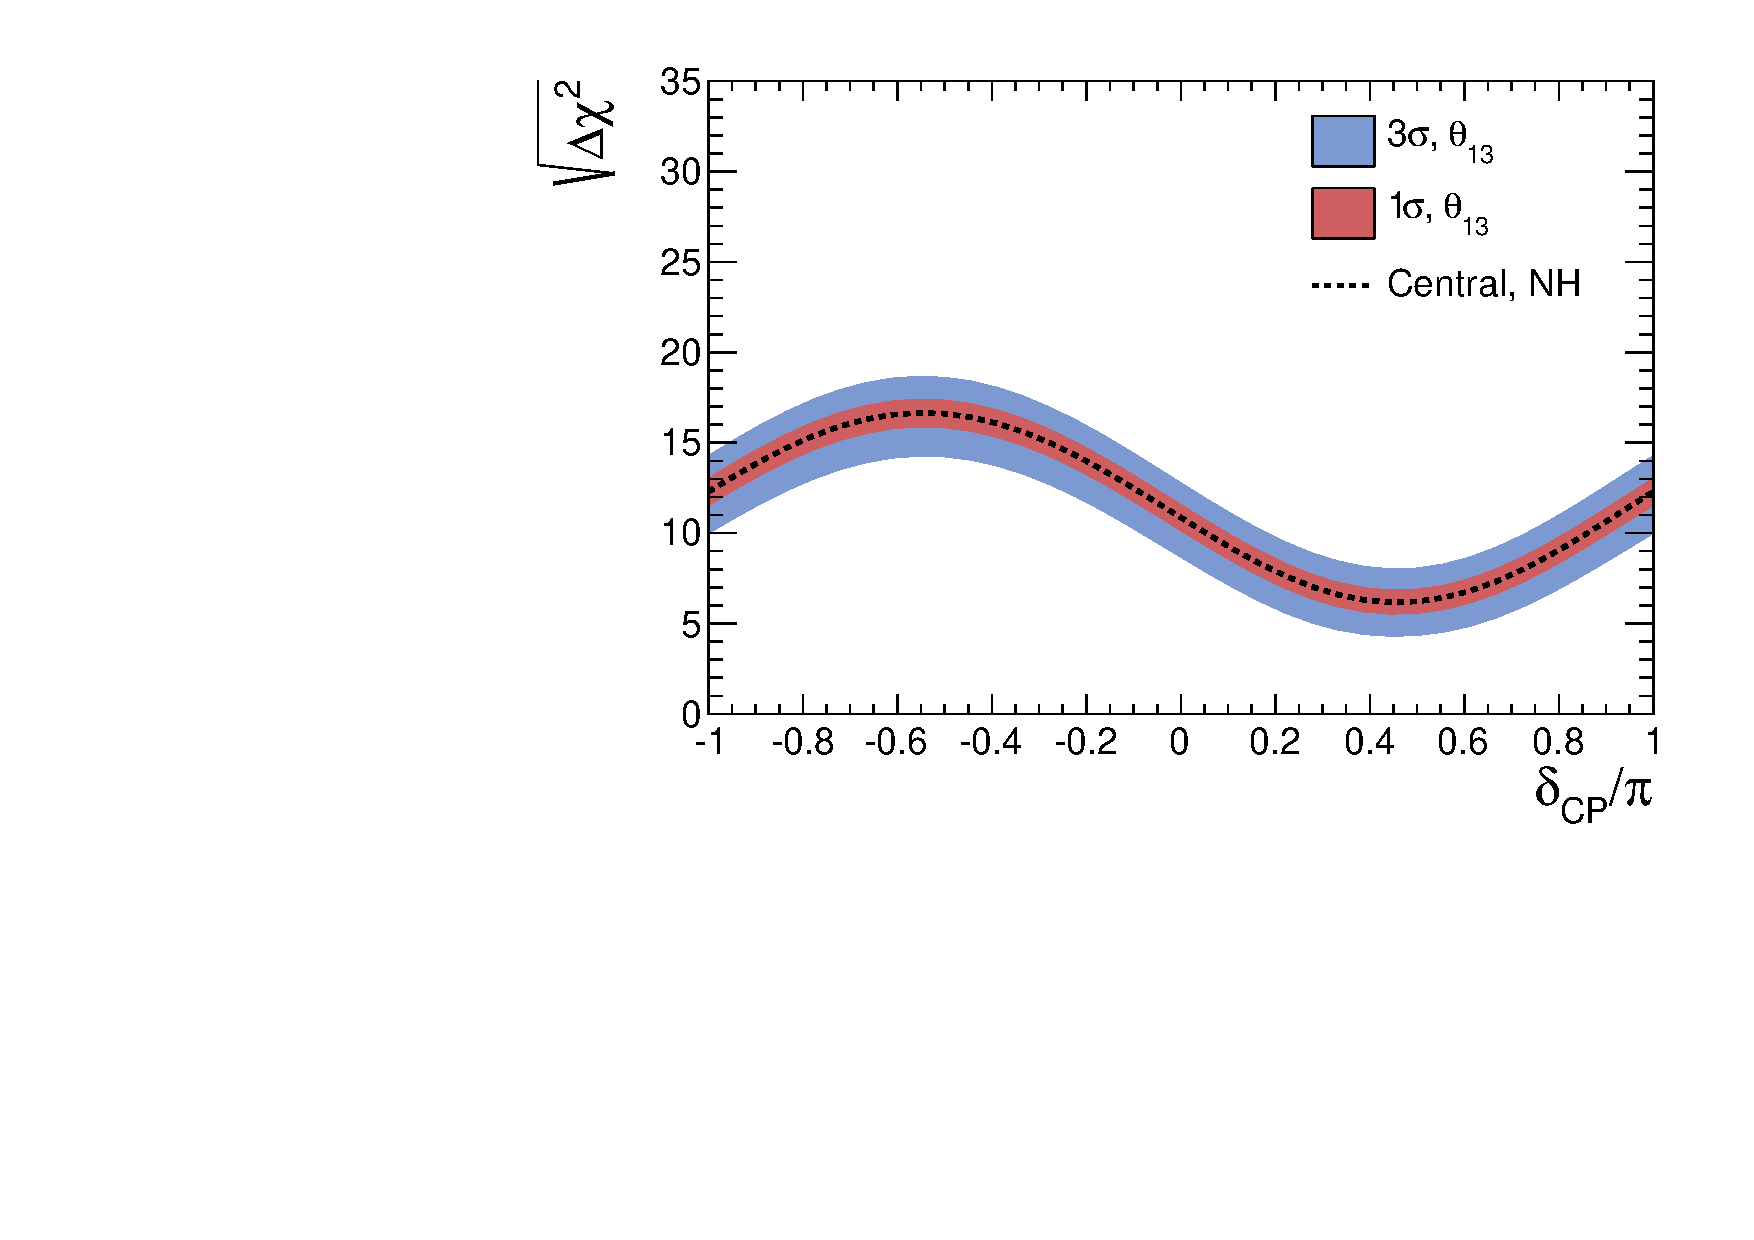
\includegraphics[width=0.45\textwidth]{figs/mh_35kt_nh_th13.pdf}
  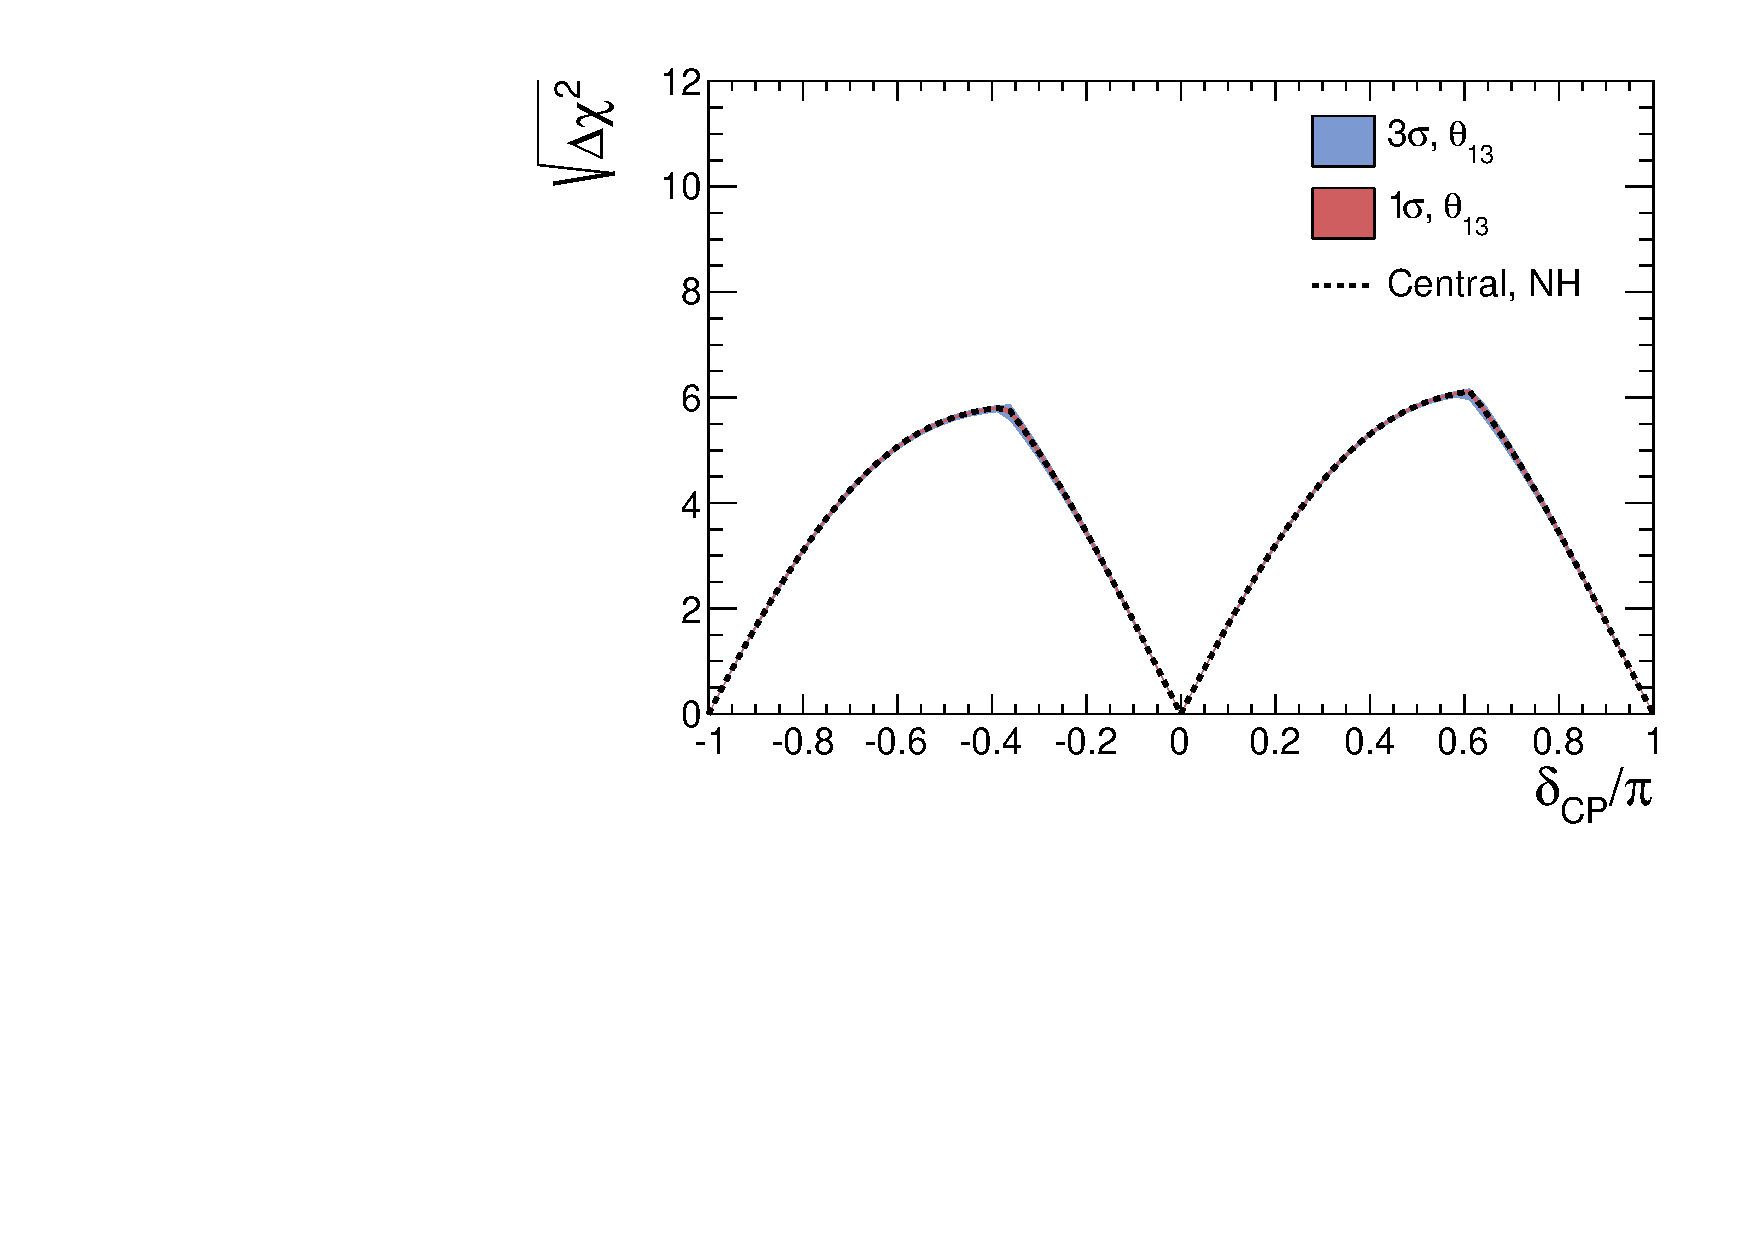
\includegraphics[width=0.45\textwidth]{figs/cpv_35kt_nh_th13.pdf}
  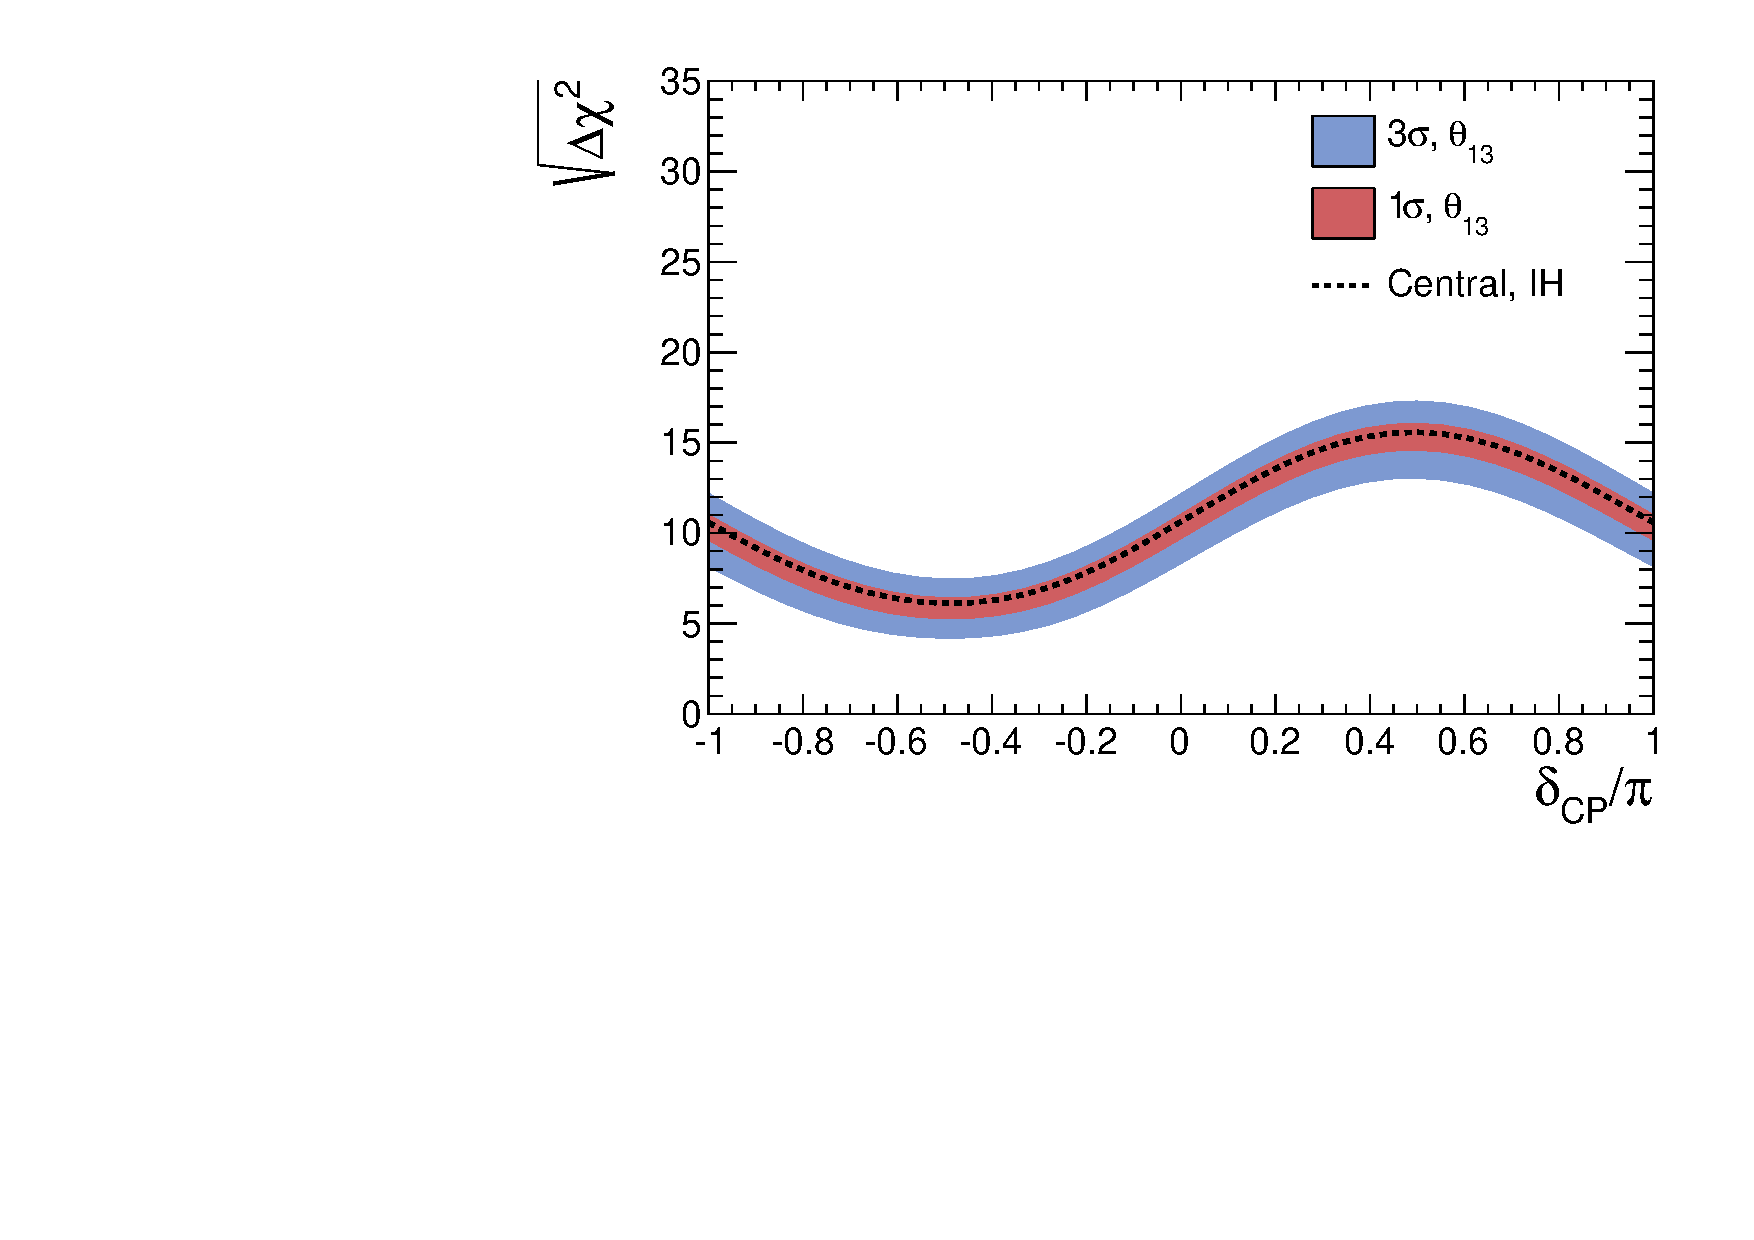
\includegraphics[width=0.45\textwidth]{figs/mh_35kt_ih_th13.pdf}
  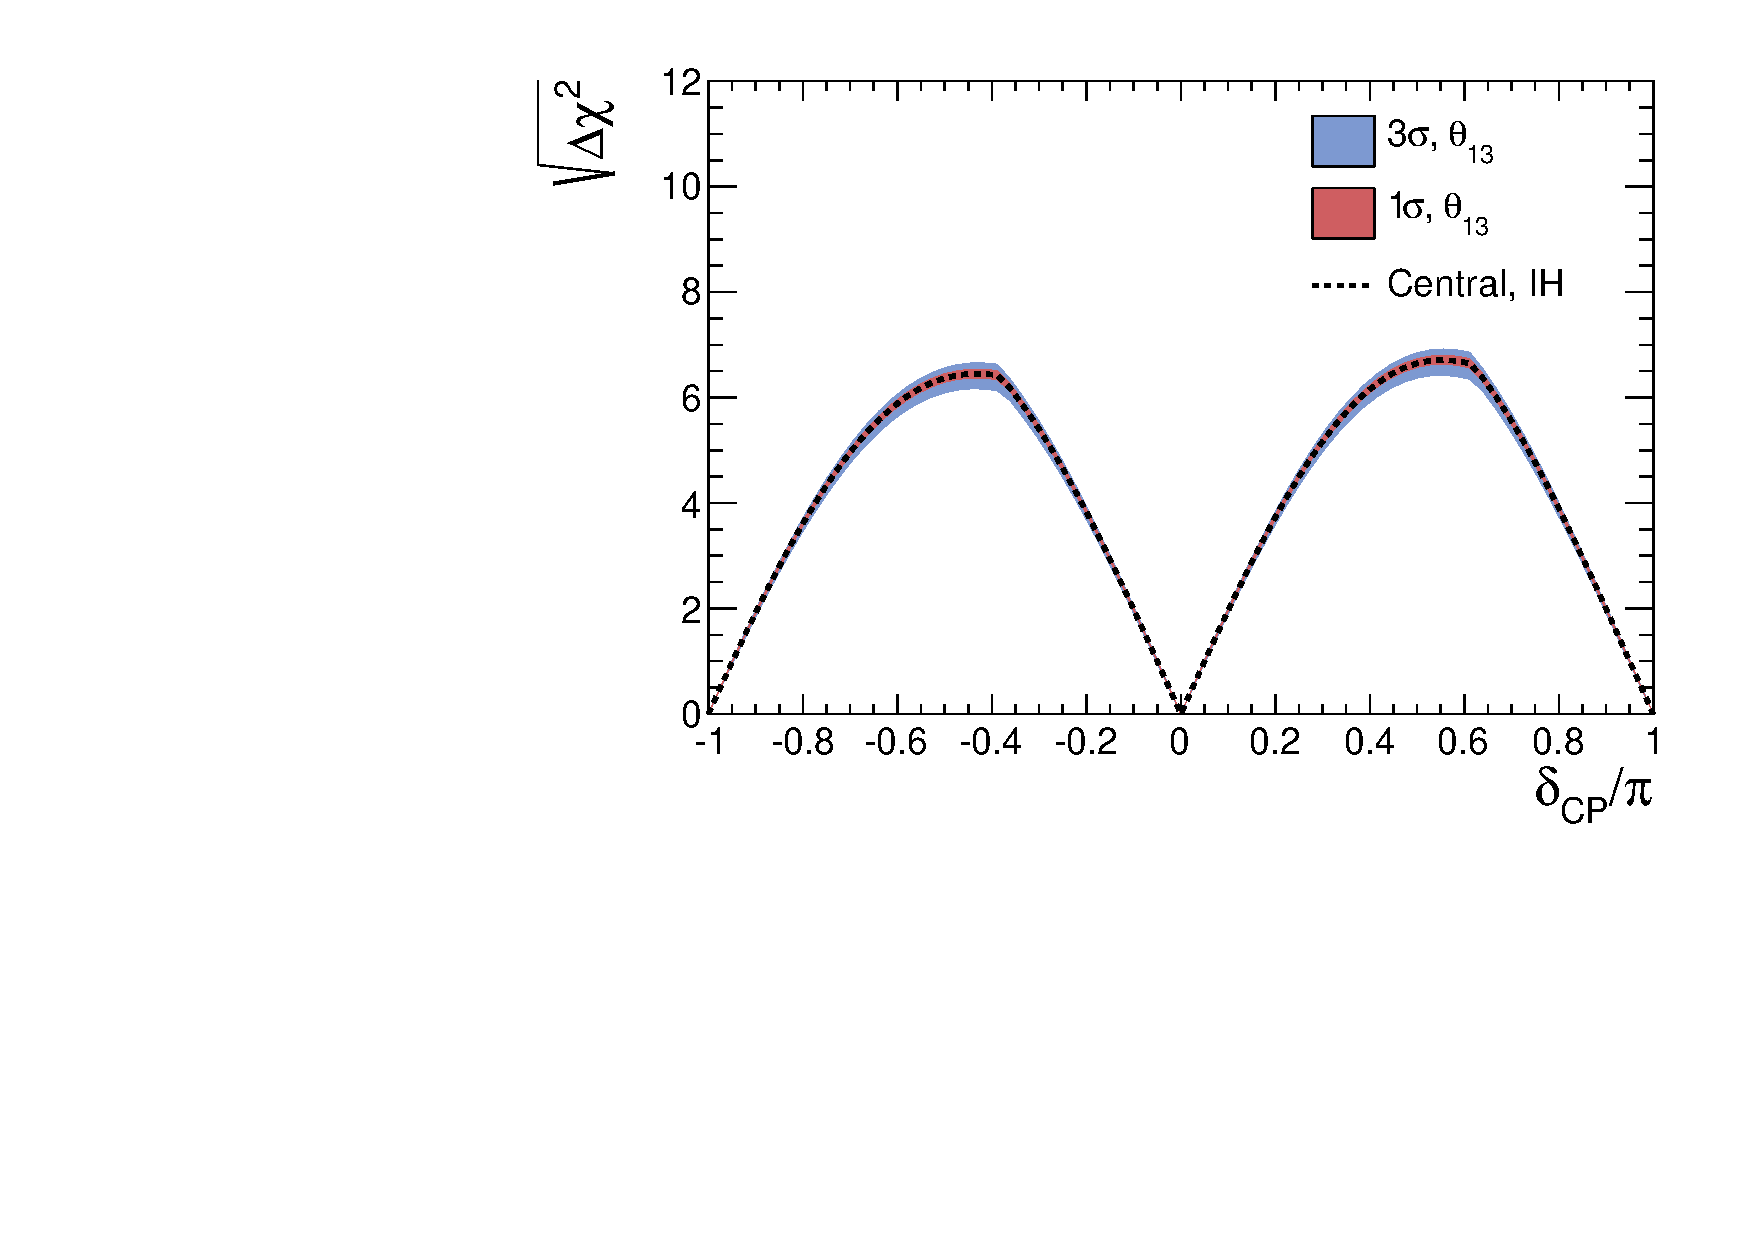
\includegraphics[width=0.45\textwidth]{figs/cpv_35kt_ih_th13.pdf}
  \caption{
  Variations in $\theta_{13}$: 
  MH (left) and CPV (right) sensitivities 
  produced by GLoBES for a 35-kt LArTPC with 3+3 ($\nu + \overline{\nu}$) years of 
  exposure in an 80-GeV, 1.2-MW beam,  for true NH (top) and true IH (bottom). 
  The effects of varying the true
  value of $\theta_{13}$ within its 1$\sigma$ (red band) and 3$\sigma$ (blue band)
  allowed ranges are shown.} 
  \label{fig:th13sens}
\end{figure}

\section{Sensitivity Dependence on $\thetatwothree$}
\label{sect:t23}

Figure \ref{fig:th23spec} shows the variation in $\nu_e$ and $\overline{\nu}_e$
appearance signal when the true value of $\theta_{23}$ is varied within its 3$\sigma$
allowed range. Increasing the true value of $\theta_{23}$ results in an increase in
$\nu_e$ appearance signal; this can be understood by inspection of 
Equation~\ref{eqn:papprox0}, where $P_0$ includes a factor of $\sin^2\theta_{23}$.
\begin{figure}[!htb]
  \centering
  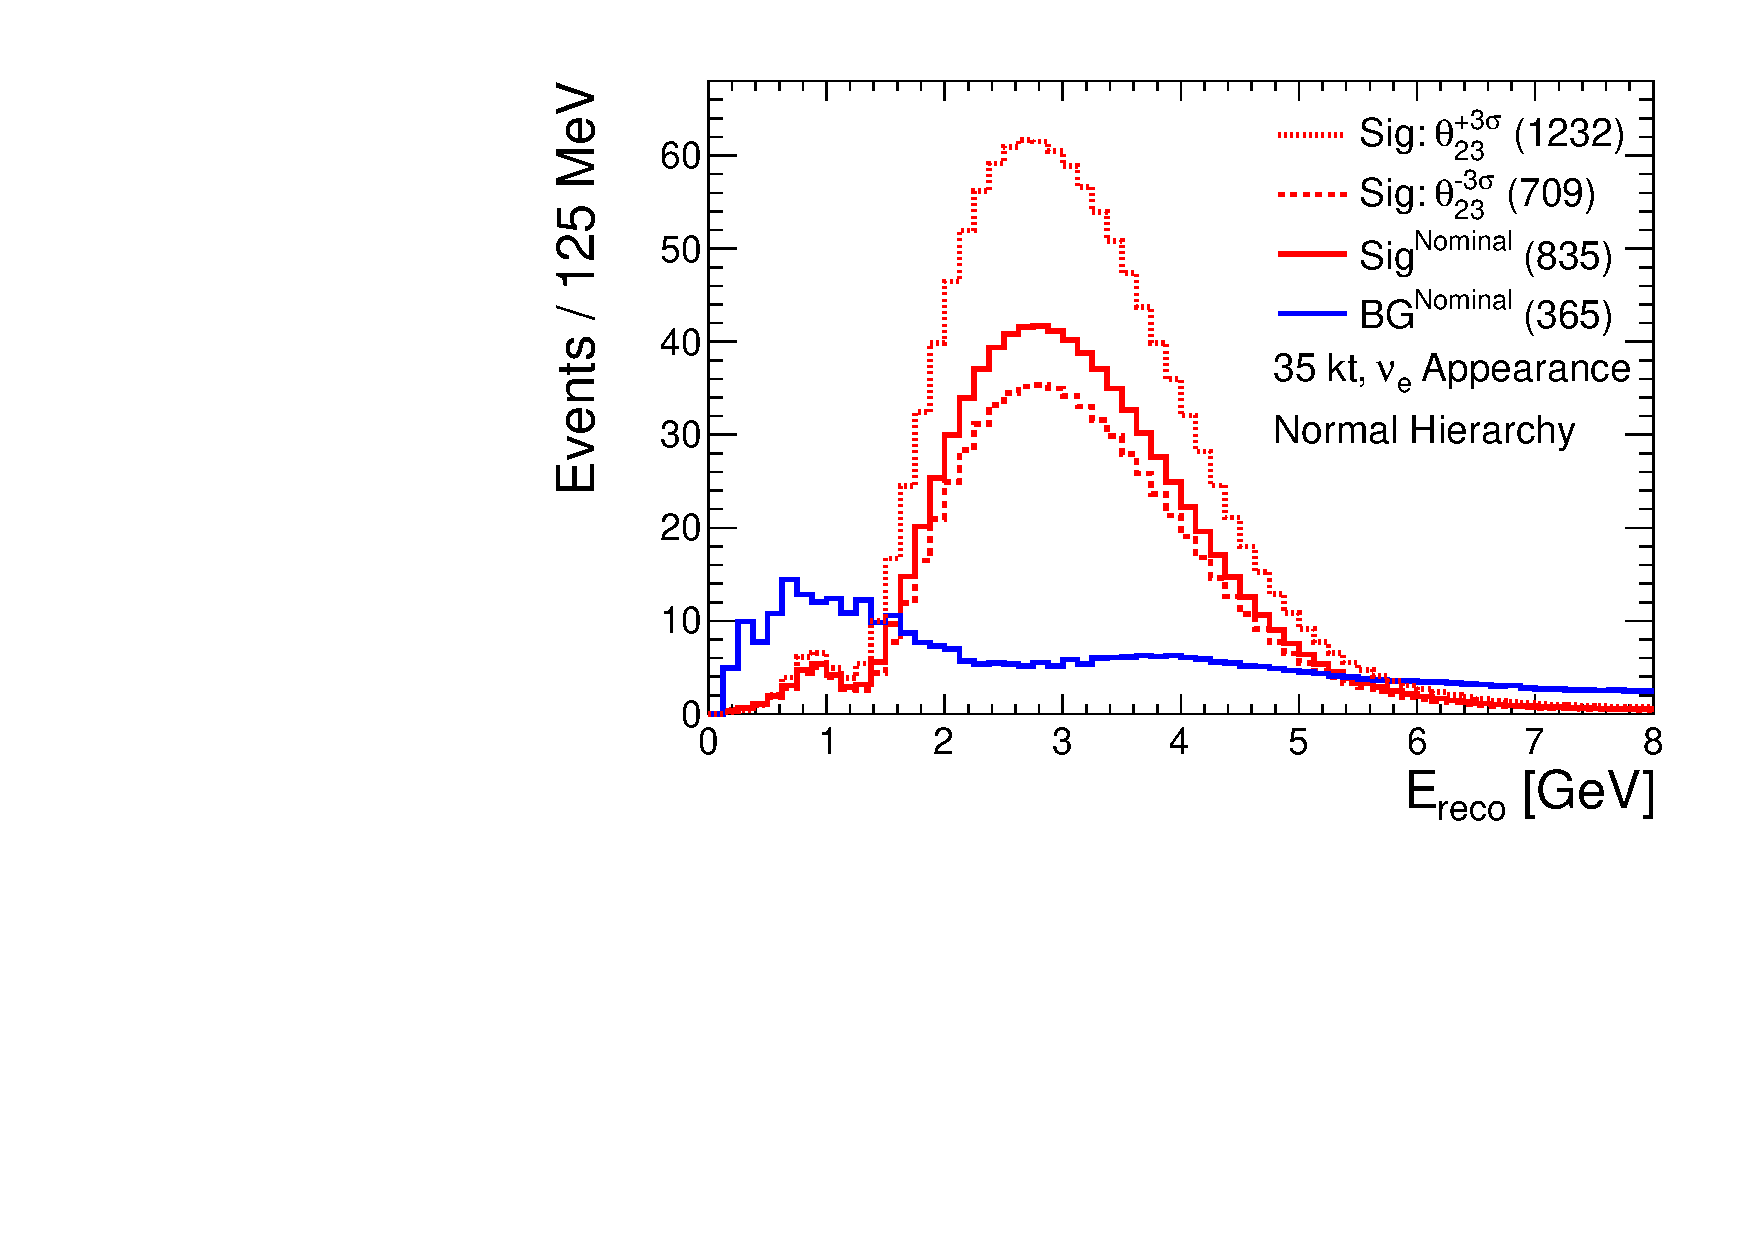
\includegraphics[width=0.45\textwidth]{figs/spectra_35kt_nue_th23var_nh.pdf}
  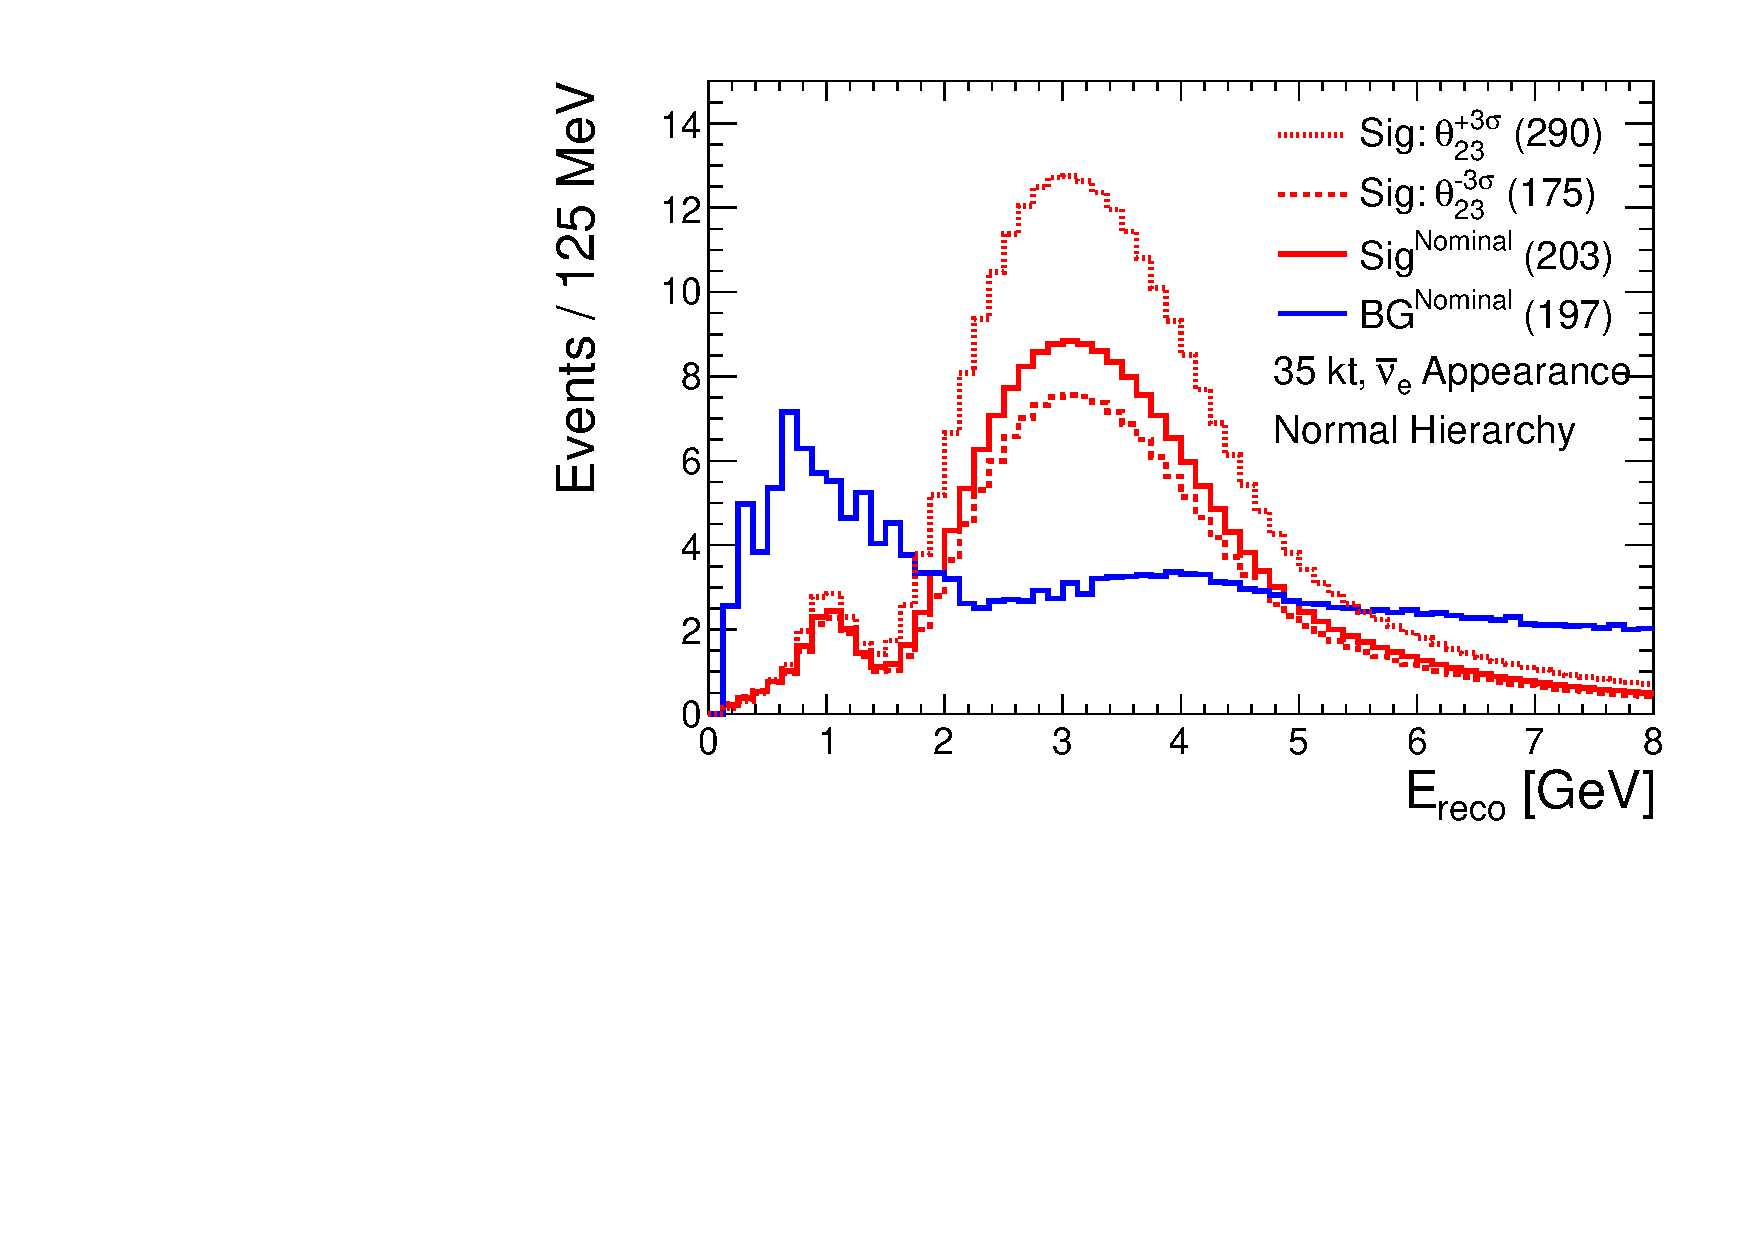
\includegraphics[width=0.45\textwidth]{figs/spectra_35kt_nuebar_th23var_nh.pdf}
  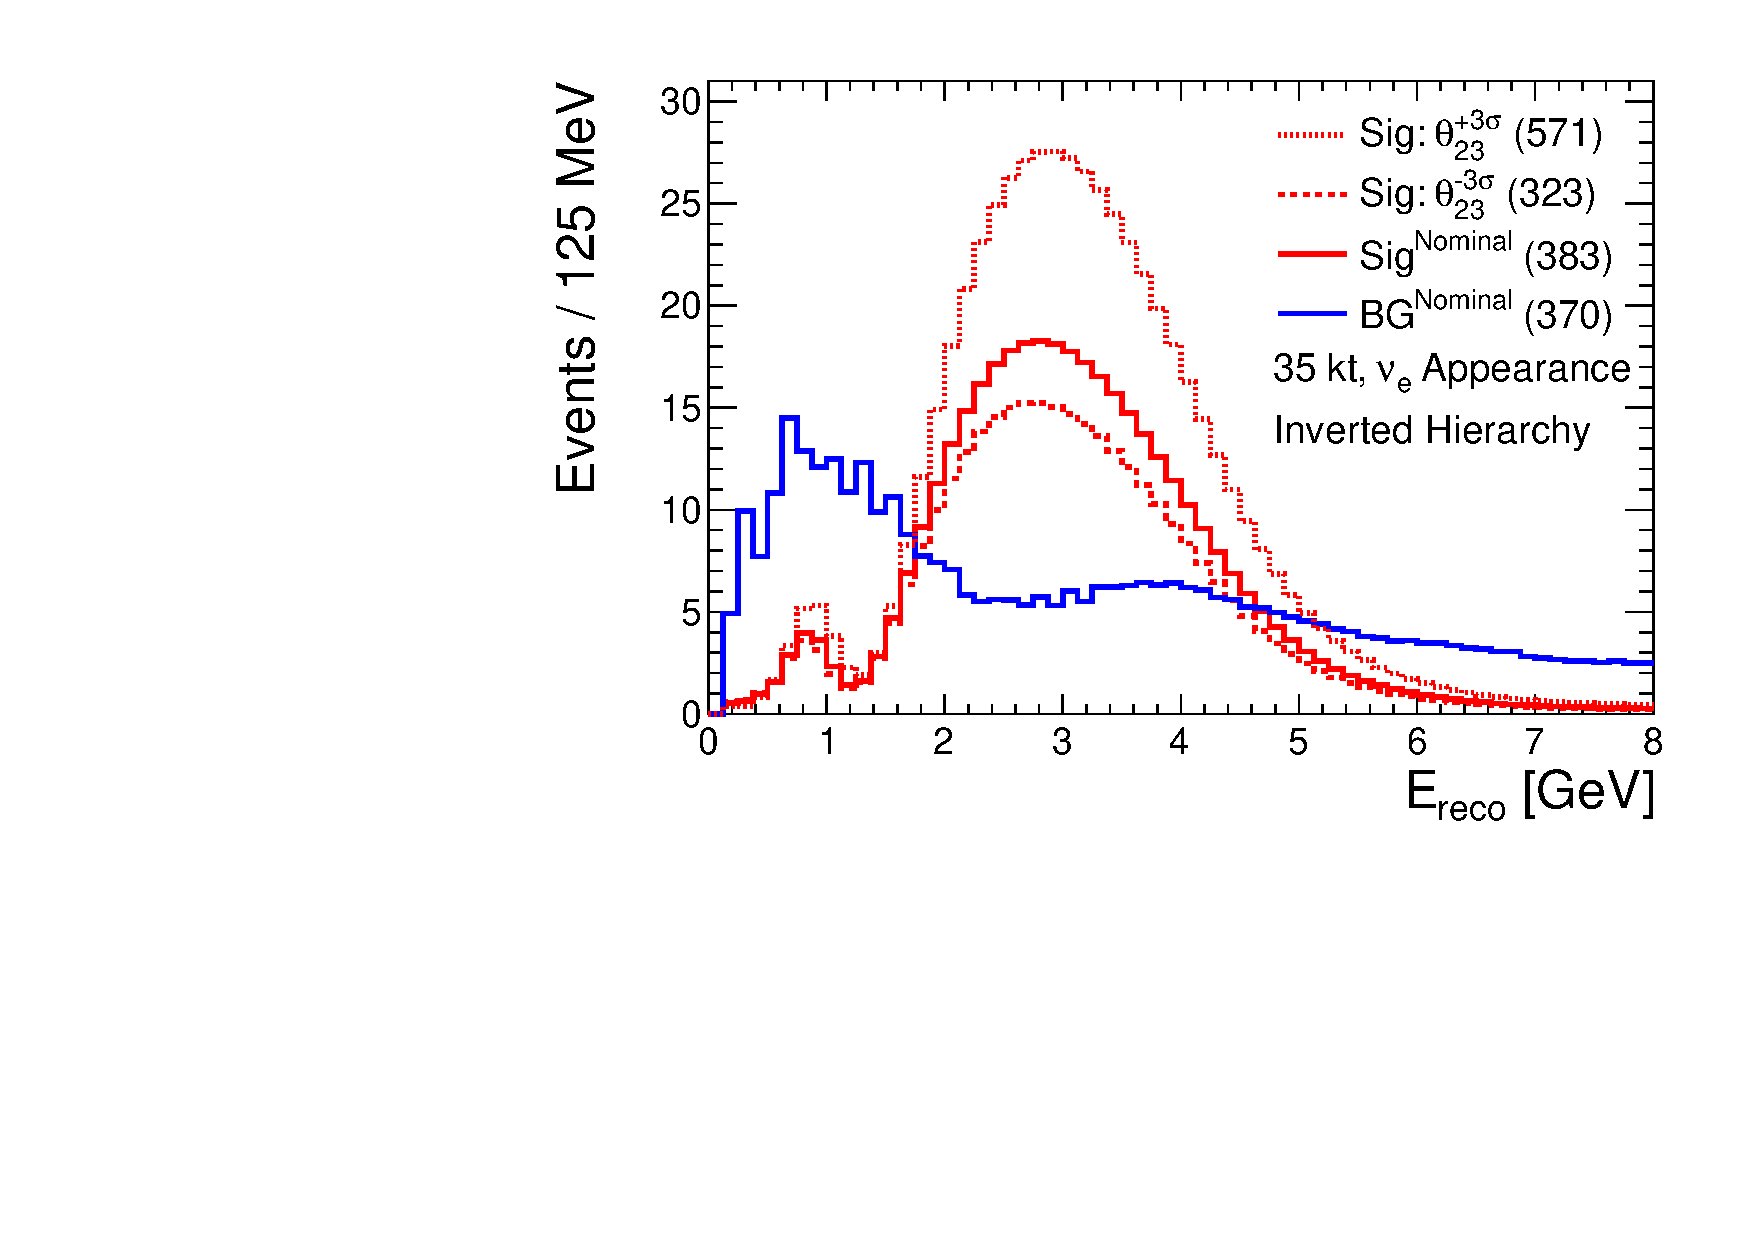
\includegraphics[width=0.45\textwidth]{figs/spectra_35kt_nue_th23var_ih.pdf}
  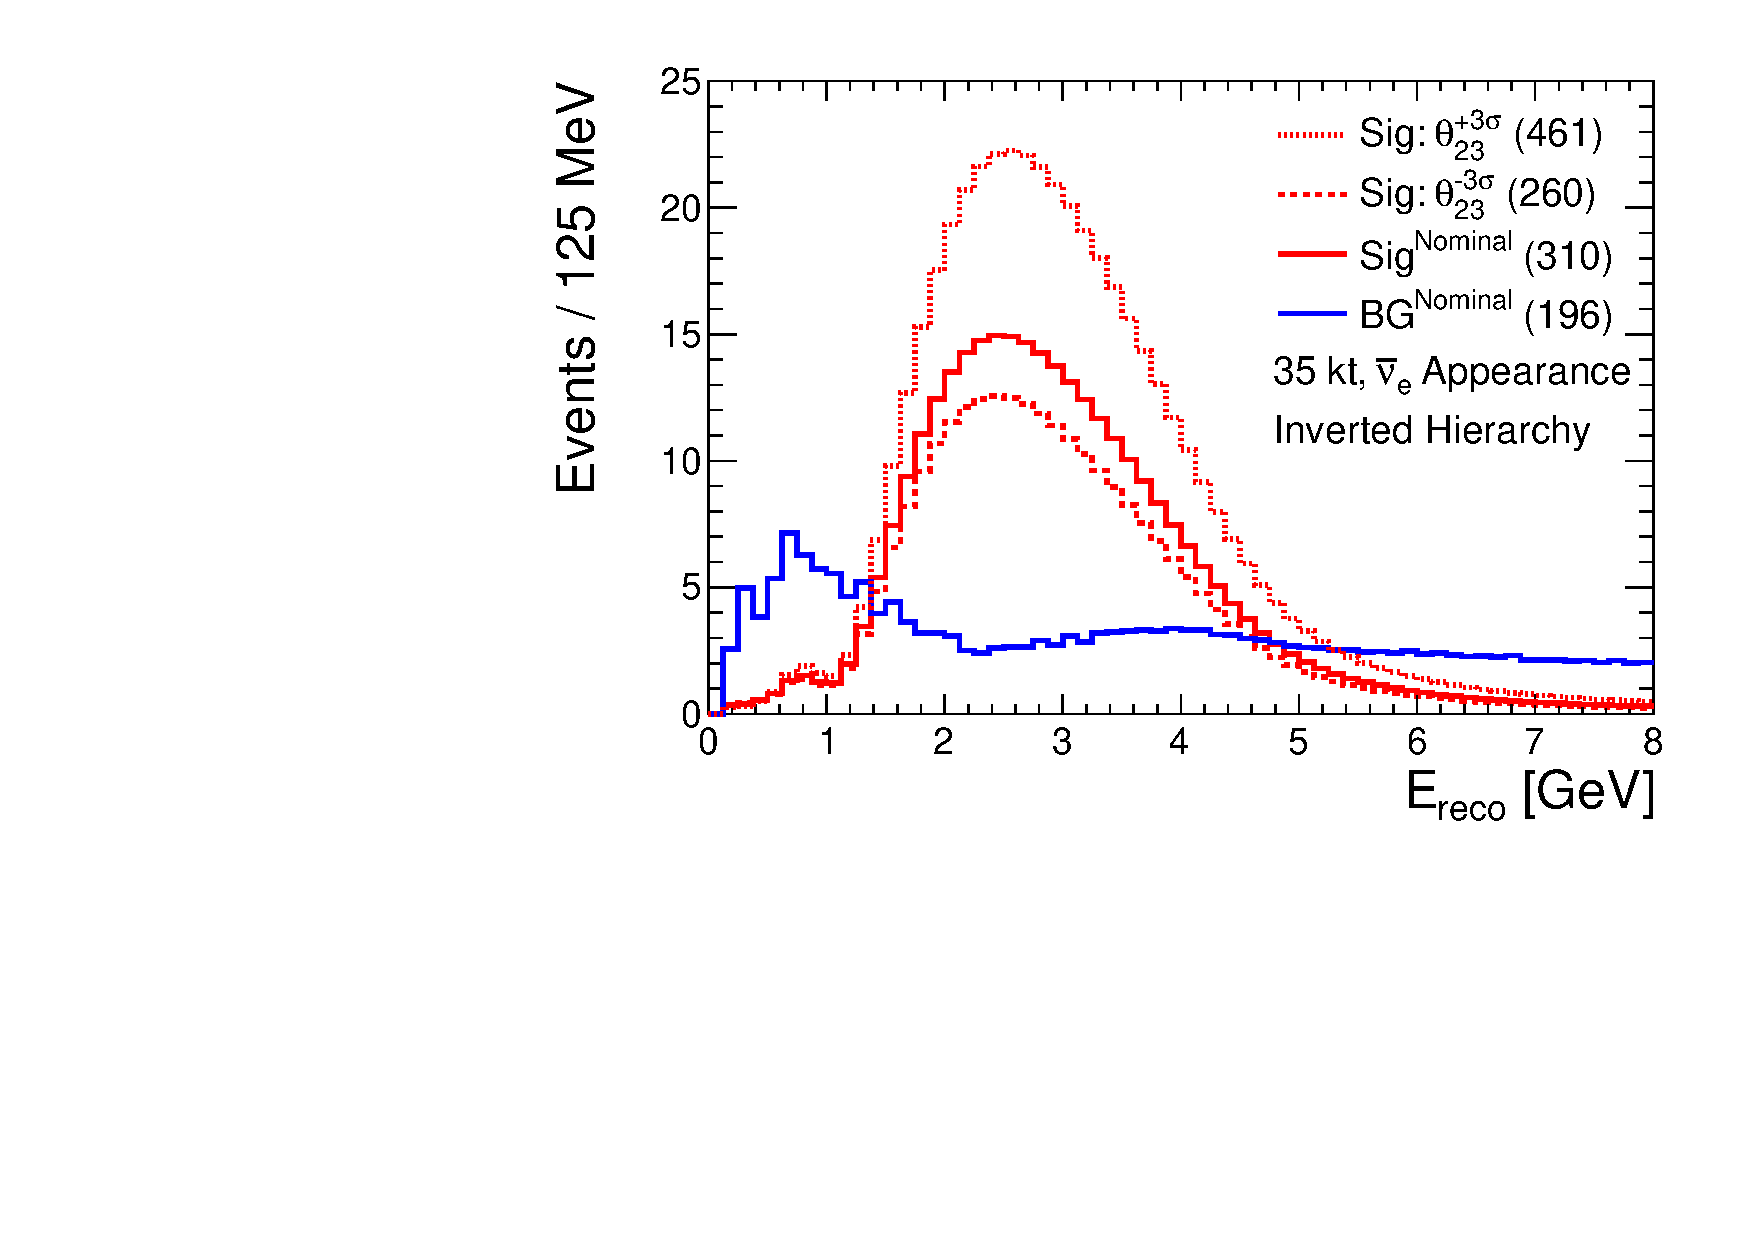
\includegraphics[width=0.45\textwidth]{figs/spectra_35kt_nuebar_th23var_ih.pdf}
  \caption{
  Variations in $\theta_{23}$:
  $\nu_e$~appearance (left) and $\overline{\nu}_e$~appearance (right) spectra 
  produced by GLoBES for a 35-kt LArTPC with 3 years of 
  exposure in an 80-GeV, 1.2-MW beam,  for true NH (top) and true IH (bottom).  
  The effect of varying the true
  value of $\theta_{23}$ within its 3$\sigma$ allowed range is shown. 
  The total background, which does not depend on value of $\theta_{23}$ (CHECKME), 
  is overlaid on the signal. The total number
  of signal and background events are indicated in parenthesis.}
  \label{fig:th23spec}
\end{figure}
Figure~\ref{fig:th23sens} shows the variation in MH and CPV sensitivity when $\theta_{23}$
is varied within its 1$\sigma$ and 3$\sigma$ allowed range. In each case, the 
nominal relative constraints on all oscillation parameters, including $\theta_{23}$, 
are applied and the normalization constraints are the nominal
1\% for signal and 5\% for background. It is clear from these figures that LBNE 
sensitivity to MH and CPV depends rather strongly on the true value of $\theta_{23}$.
As $\theta_{23}$ increases, sensitivity to CPV decreases while sensitivity to
MH increases. Starting from Equation~\ref{eqn:papprox0}, one can show
that the CP asymmetry measured by LBNE depends directly on
$\theta_{23}$:
\begin{equation}
\mathcal{A}_{CP} \sim \frac{\cos \theta_{23} \sin 2 \theta_{12}
  {\sin \delta_{CP}}}{\sin \theta_{23} \sin \theta_{13}}
\left(\frac{\Delta m^2_{21} L}{ 4 E_{\nu}}\right) + {\rm matter
  \ effects}.
\end{equation}
This asymmetry decreases with increasing $\theta_{23}$; sensitivity decreases
because the quantity being measured is smaller. The decrease in CP asymmetry also
explains the increase in MH sensitivity. The limiting factor to MH sensitivity
in the region where $\delta_{CP}>0$ is the degeneracy between CP and matter
asymmetries, described in Section~\ref{sect:nuosc}. The decrease in CP asymmetry
with increasing $\theta_{23}$ partially breaks this degeneracy, increasing MH
sensitivity. This effect is illustrated by the spectra in Fig.~\ref{fig:degspec}.
The explicit dependence of the MH sensitivity on $\theta_{23}$ is shown in 
Fig.~\ref{fig:mh_th23_dependance}.
%
\begin{figure}[!htb]
  \centering
  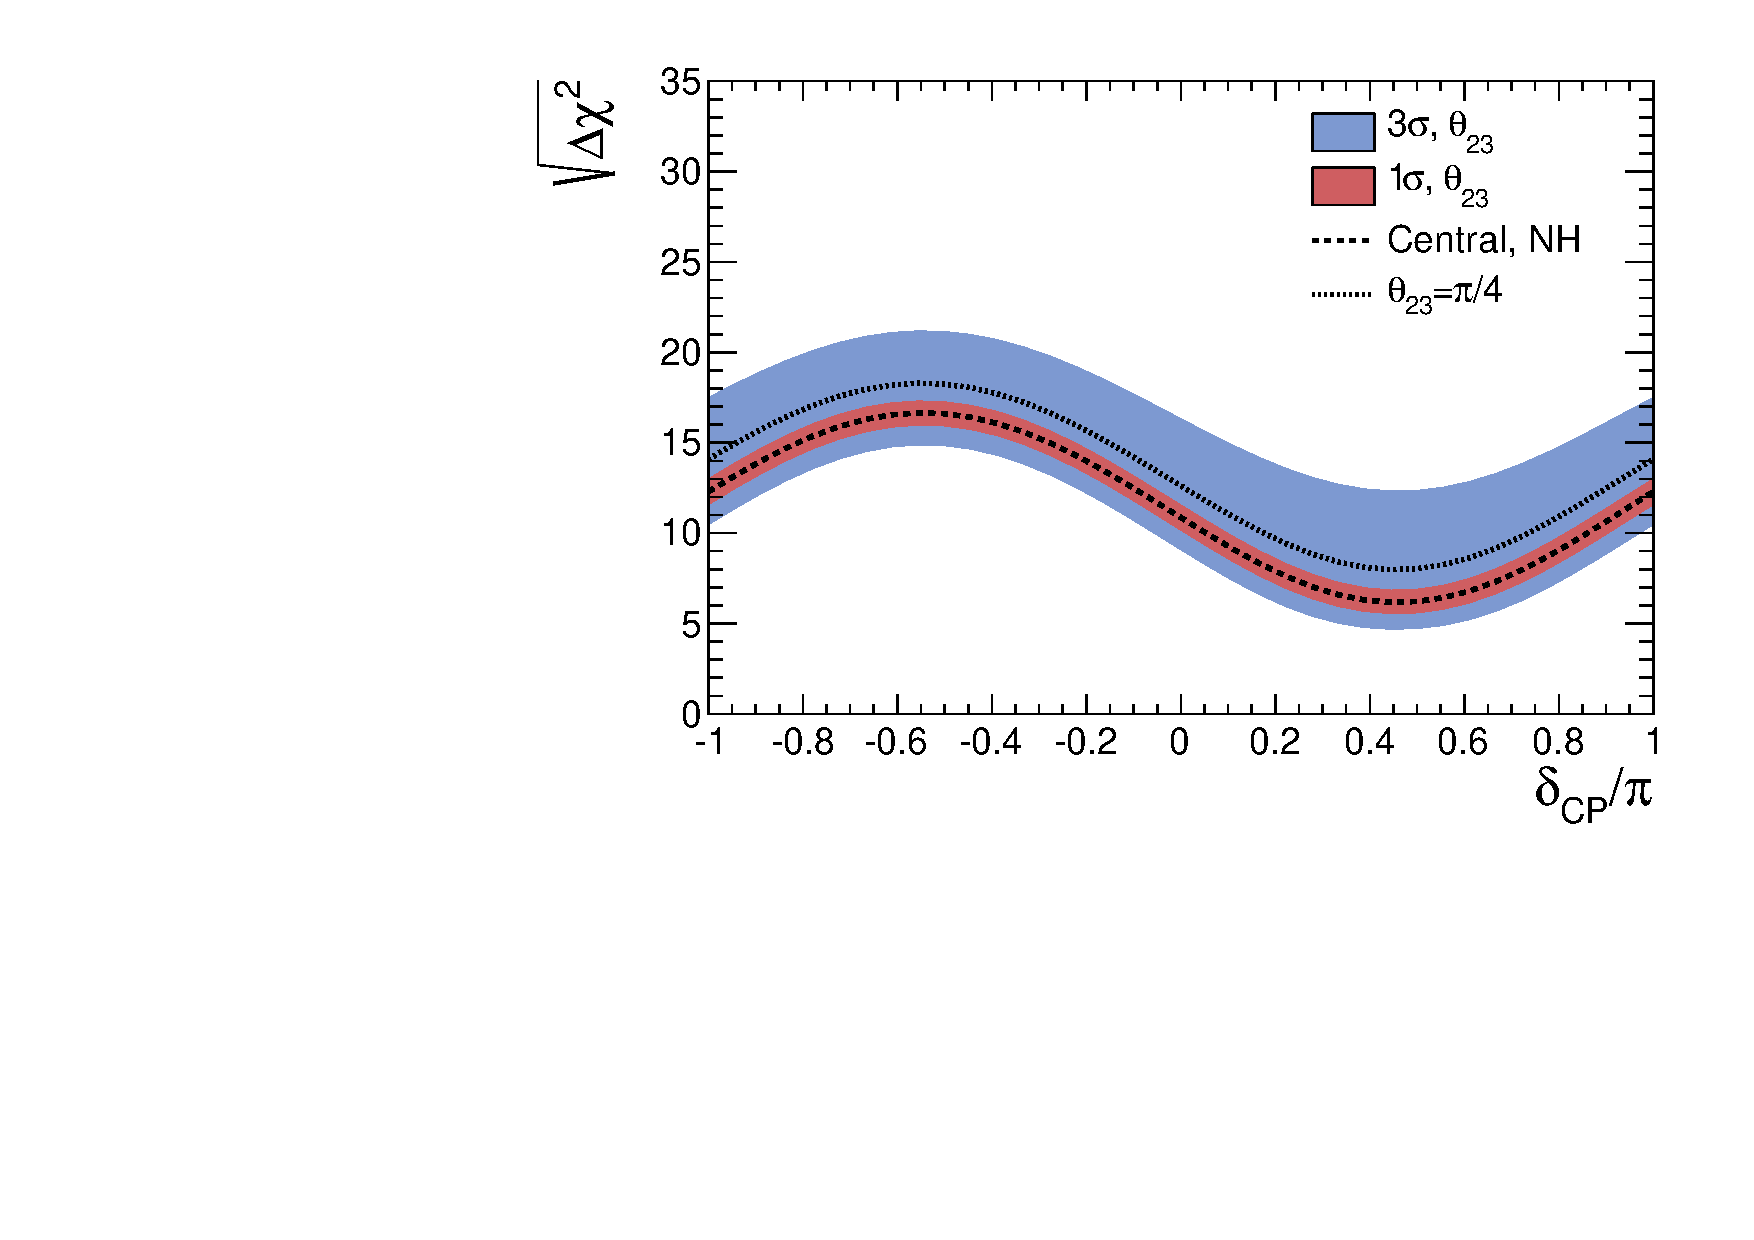
\includegraphics[width=0.45\textwidth]{figs/mh_35kt_nh_th23.pdf}
  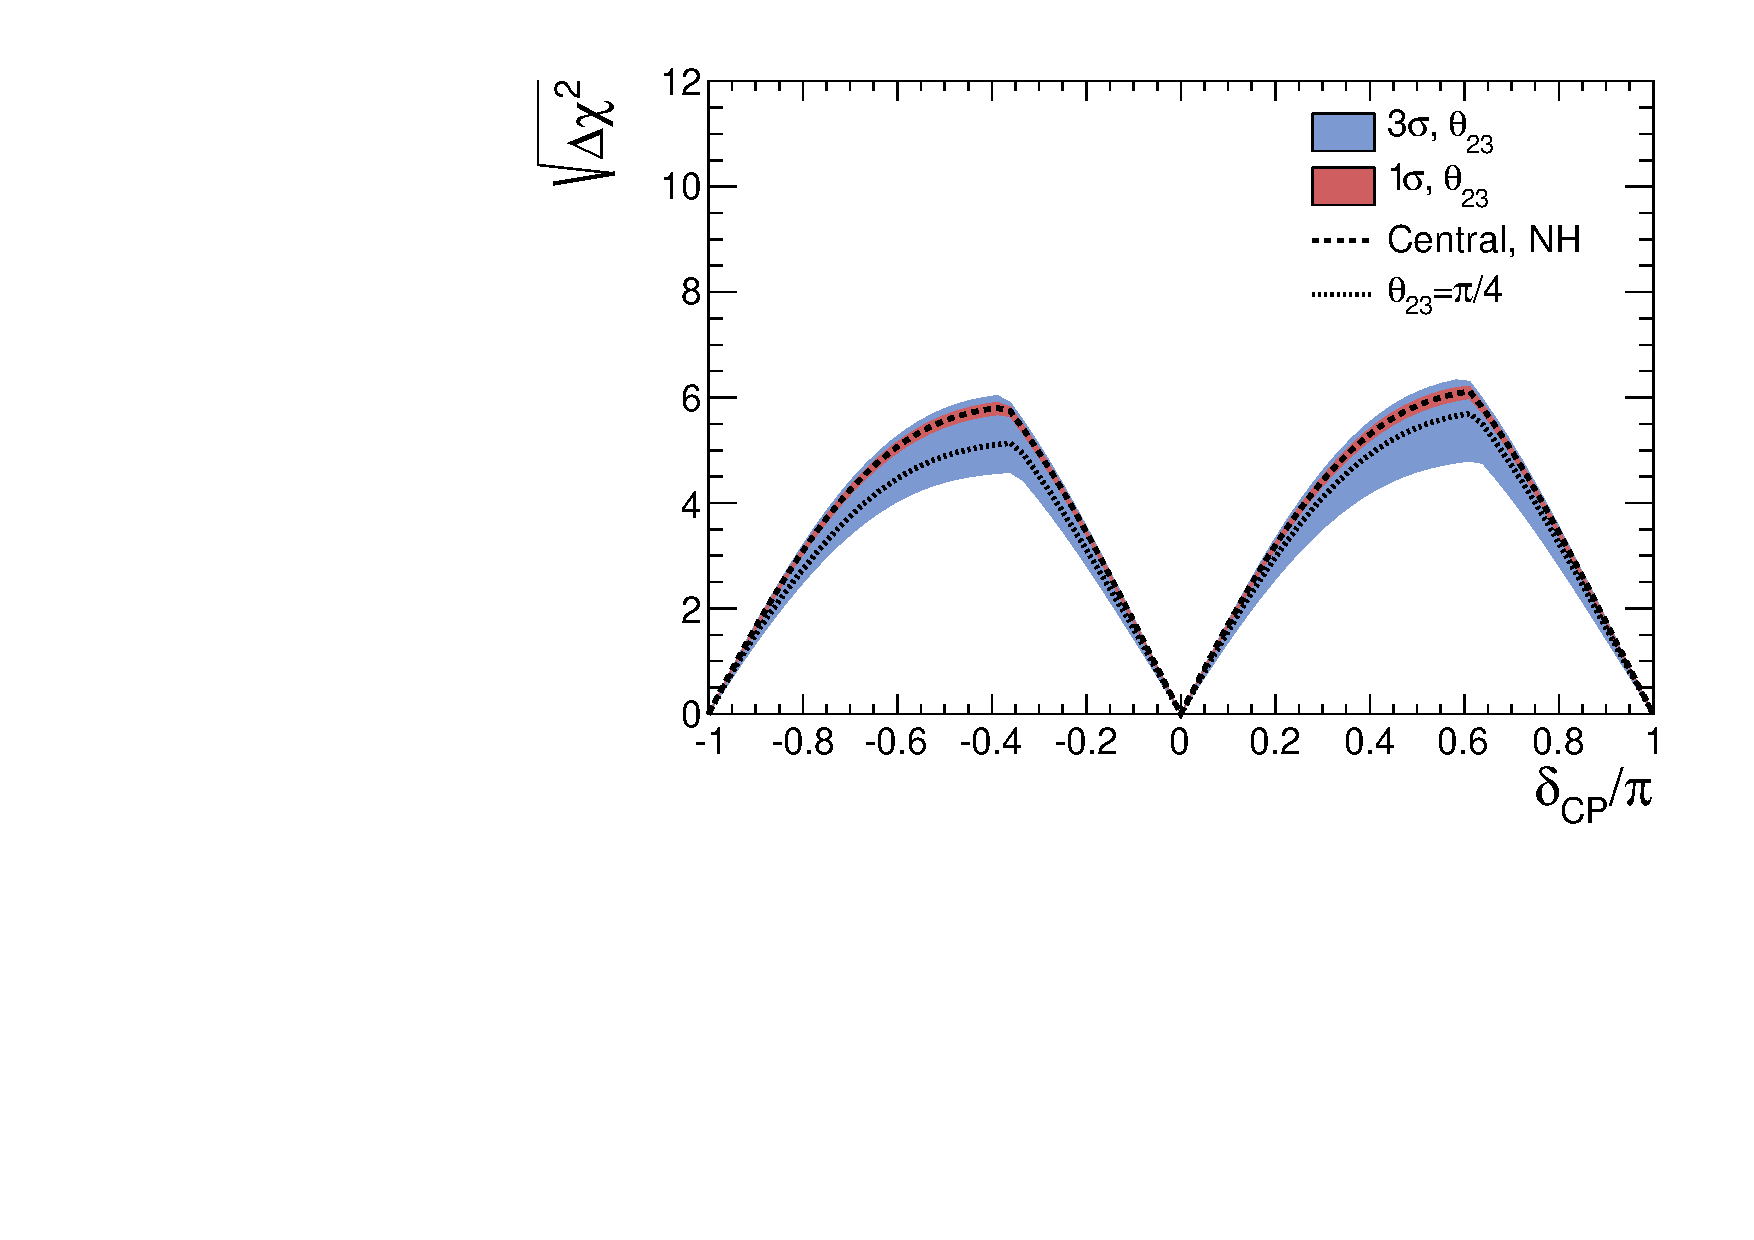
\includegraphics[width=0.45\textwidth]{figs/cpv_35kt_nh_th23.pdf}
  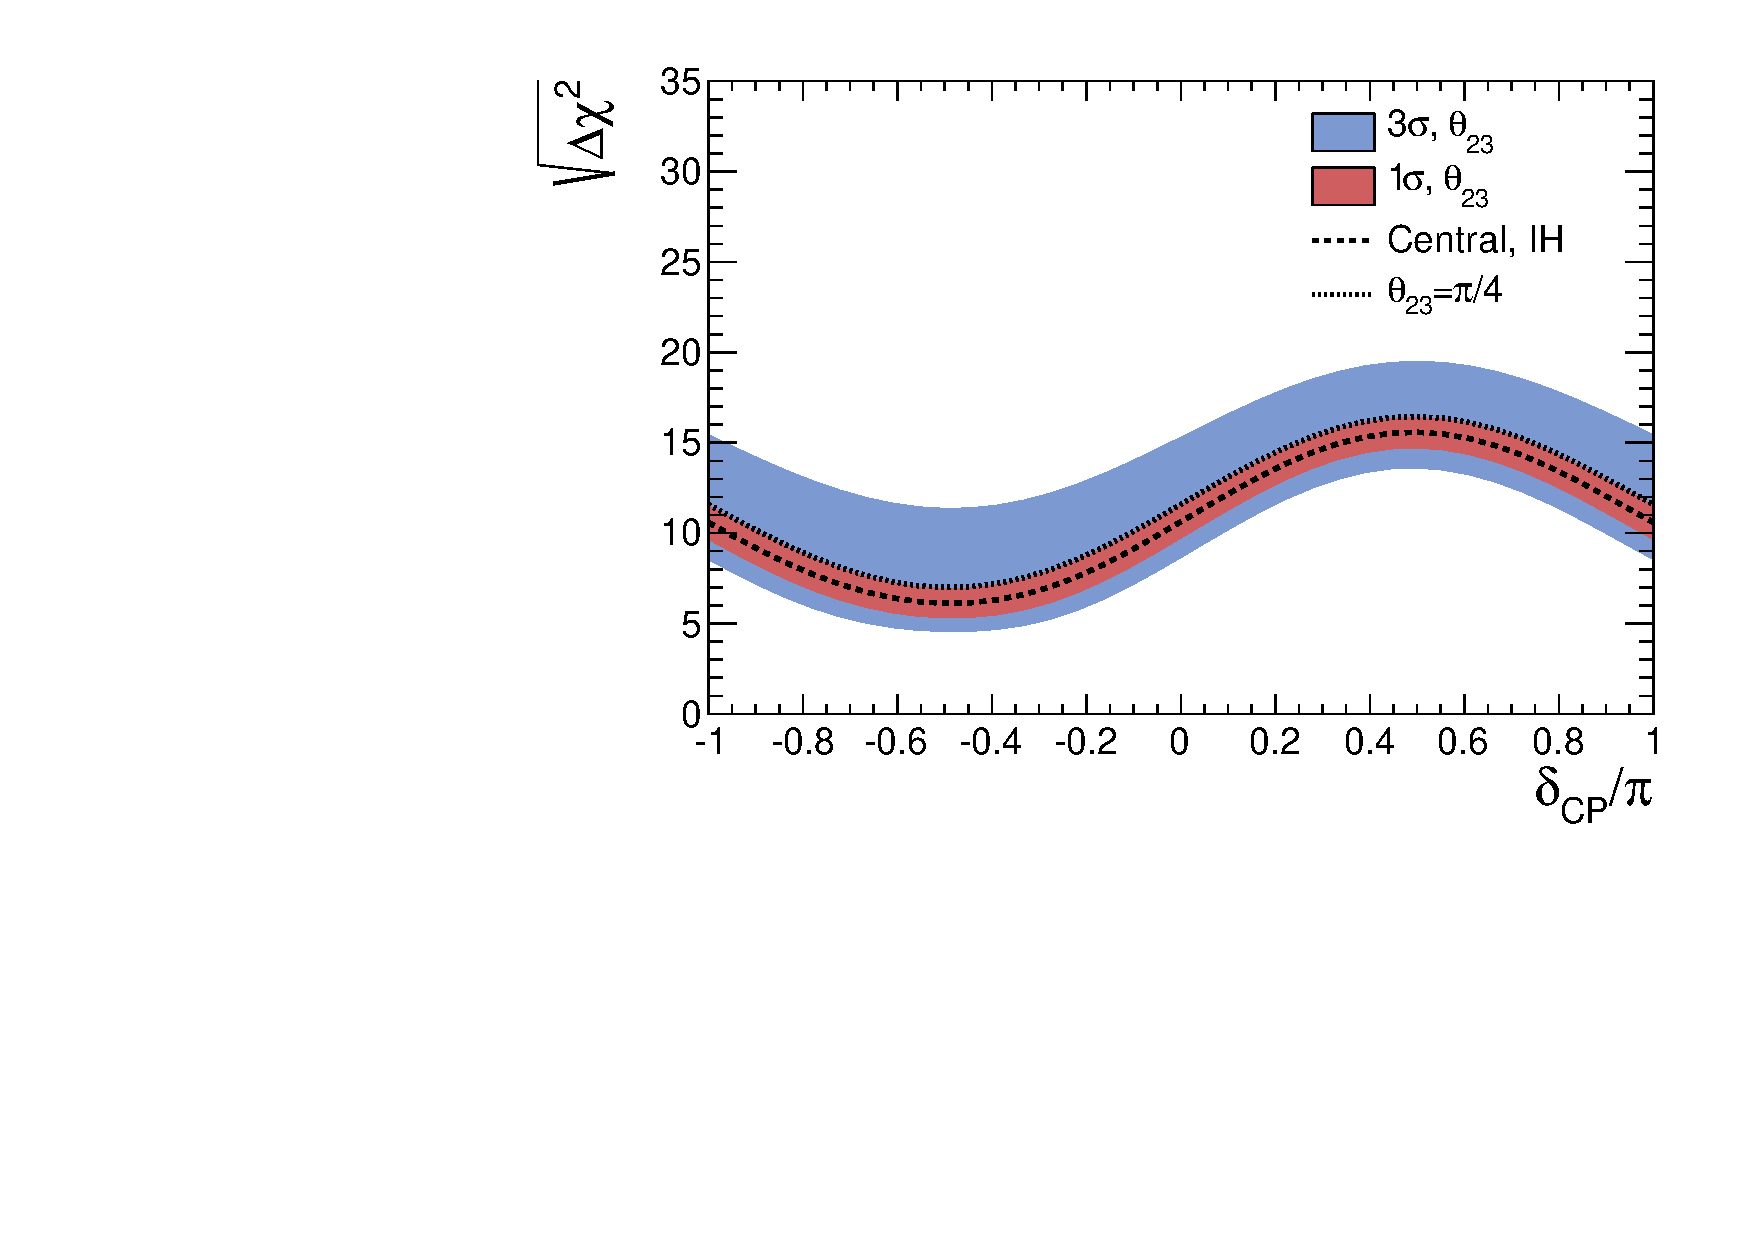
\includegraphics[width=0.45\textwidth]{figs/mh_35kt_ih_th23.pdf}
  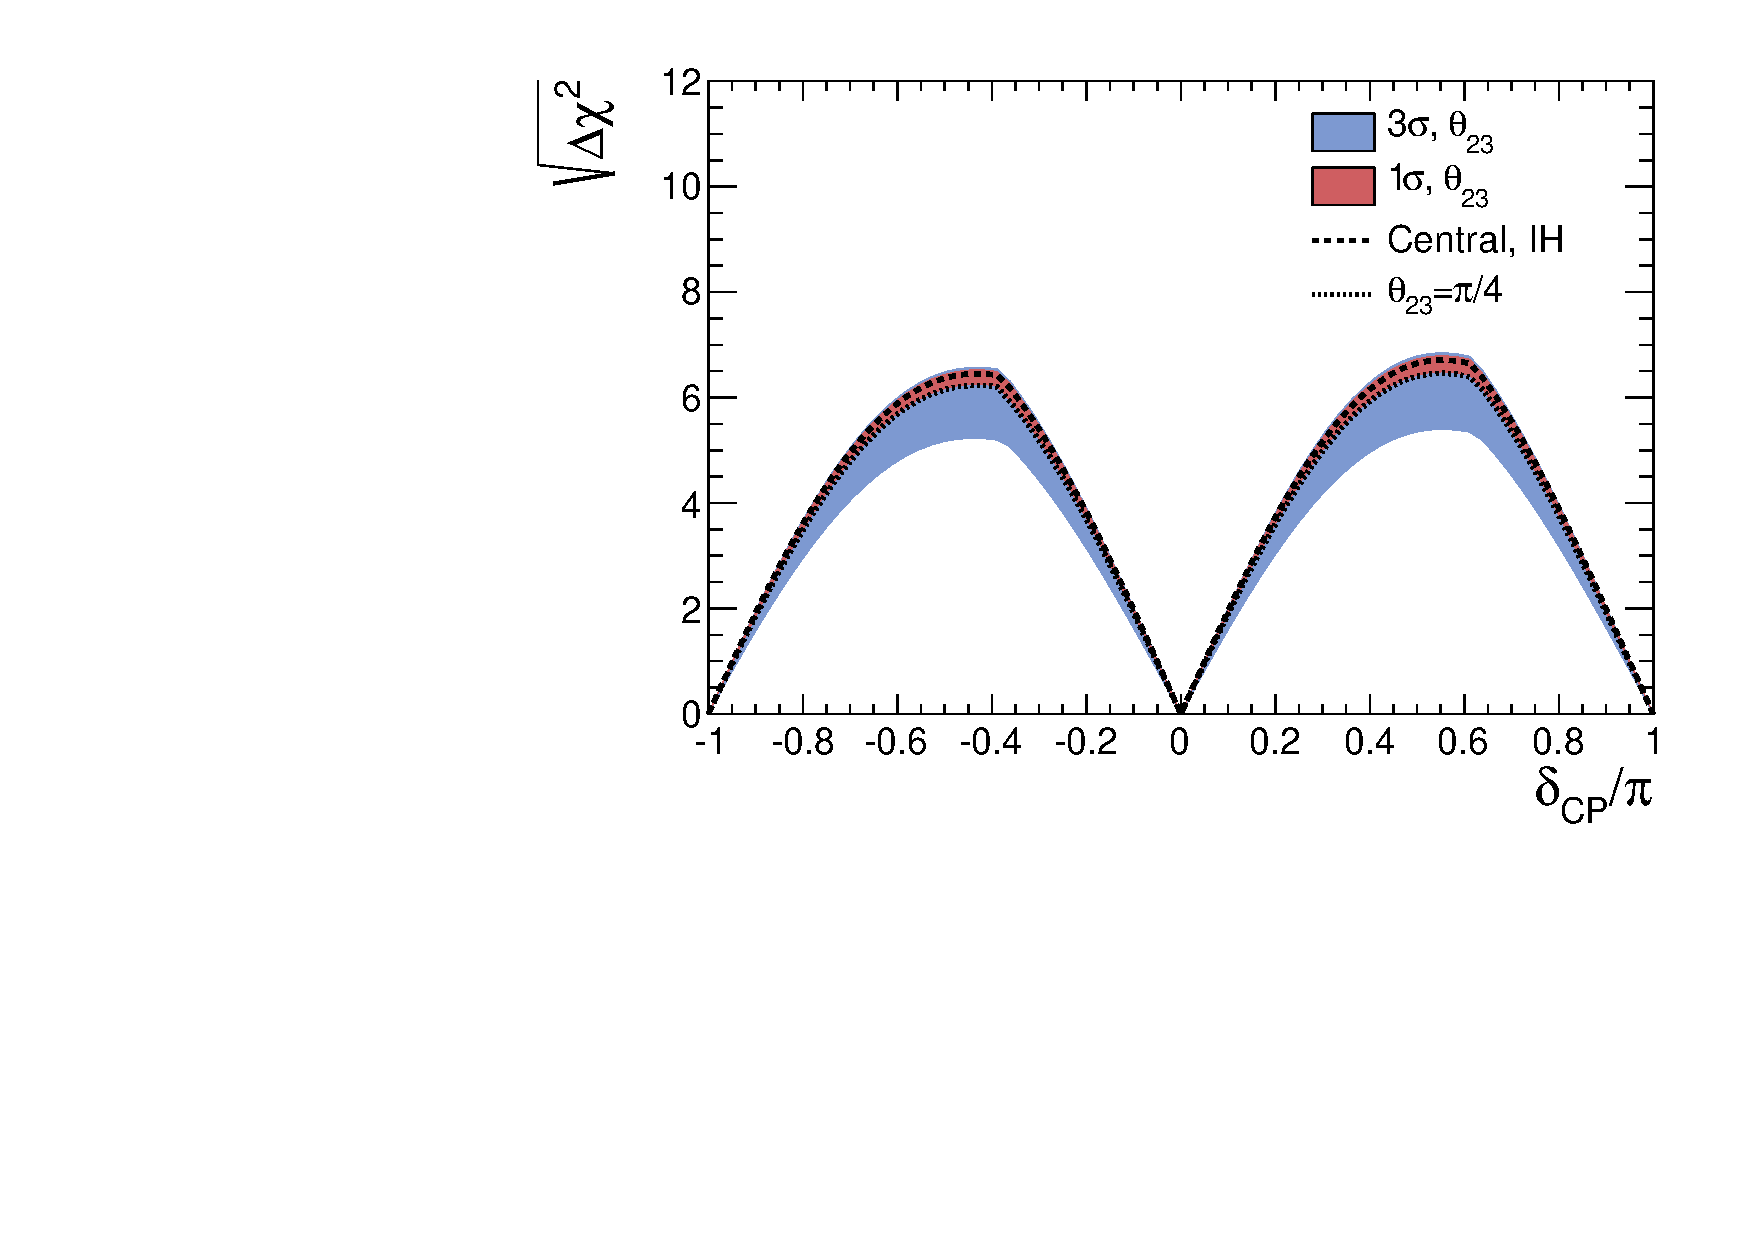
\includegraphics[width=0.45\textwidth]{figs/cpv_35kt_ih_th23.pdf}
  \caption{
  Variations in $\theta_{23}$: 
  MH (left) and CPV (right) sensitivities 
  produced by GLoBES for a 35-kt LArTPC with 3+3 ($\nu + \overline{\nu}$) years of 
  exposure in an 80-GeV, 1.2-MW beam,  for true NH (top) and true IH (bottom). 
  The effects of varying the true
  value of $\theta_{23}$ within its 1$\sigma$ (red band) and 3$\sigma$ (blue band)
  allowed ranges are shown. The sensitivities when $\theta_{23} = \pi/4$ (maximal
  mixing between $\nu_{\mu}$ and $\nu_{\tau}$) are also shown.} 
  \label{fig:th23sens}
\end{figure}
%
\begin{figure}[!htbp]
\centering
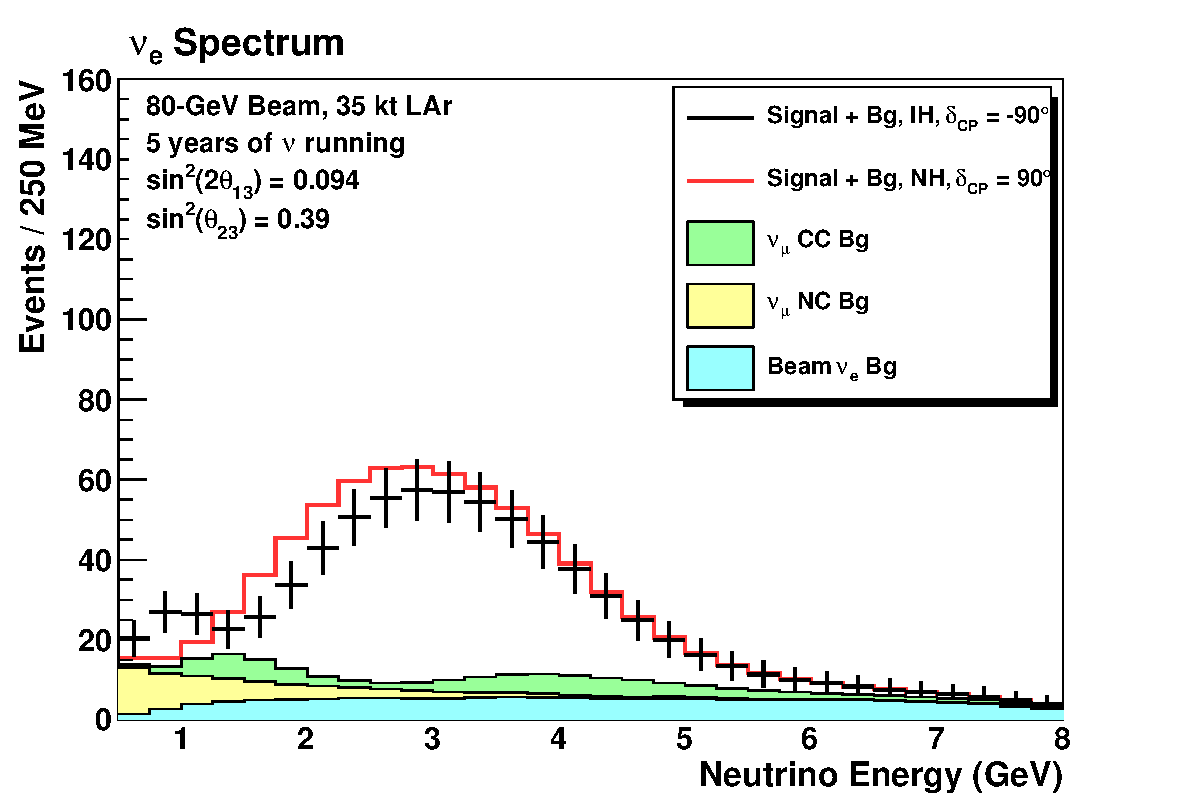
\includegraphics[width=0.45\linewidth]{figs/spec_nh90_ih-90_80gev.pdf}
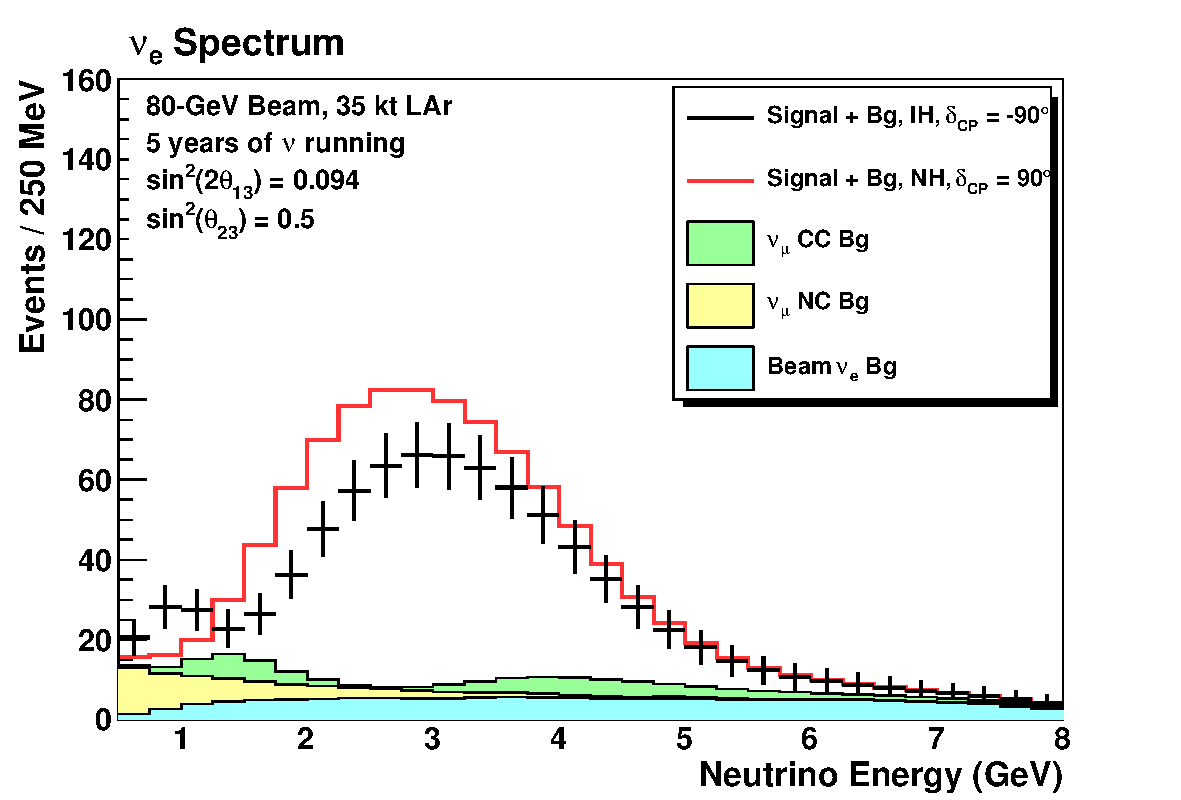
\includegraphics[width=0.45\linewidth]{figs/spec_nh90_ih-90_80gev_th23max.pdf}
\caption{Spectrum for true normal hierarchy and $\dcp=\pi/2$ (red) compared to the
spectrum for true inverted hierarchy and $\dcp=-\pi/2$ (black), 
for $\sthetatwothree=0.39$
(left) and $\sthetatwothree=0.5$ (right). For the smaller value of $\thetatwothree$
shown on the left, the spectra are quite degenerate. For the larger value 
of $\thetatwothree$ shown on the right, the degeneracy is broken.
Neutrino event spectra are shown for illustration; the degeneracy is also broken
in antineutrino spectra.}
\label{fig:degspec}
\end{figure}

\section{Sensitivity Dependence on $\Dmsq$}
\label{sect:Dmsq}

Figure \ref{fig:dmspec} shows the variation in $\nu_e$ and $\overline{\nu}_e$
appearance signal when the true value of $\Delta m^2_{31}$ is varied within its 3$\sigma$
allowed range. 
\begin{figure}[!htb]
  \centering
  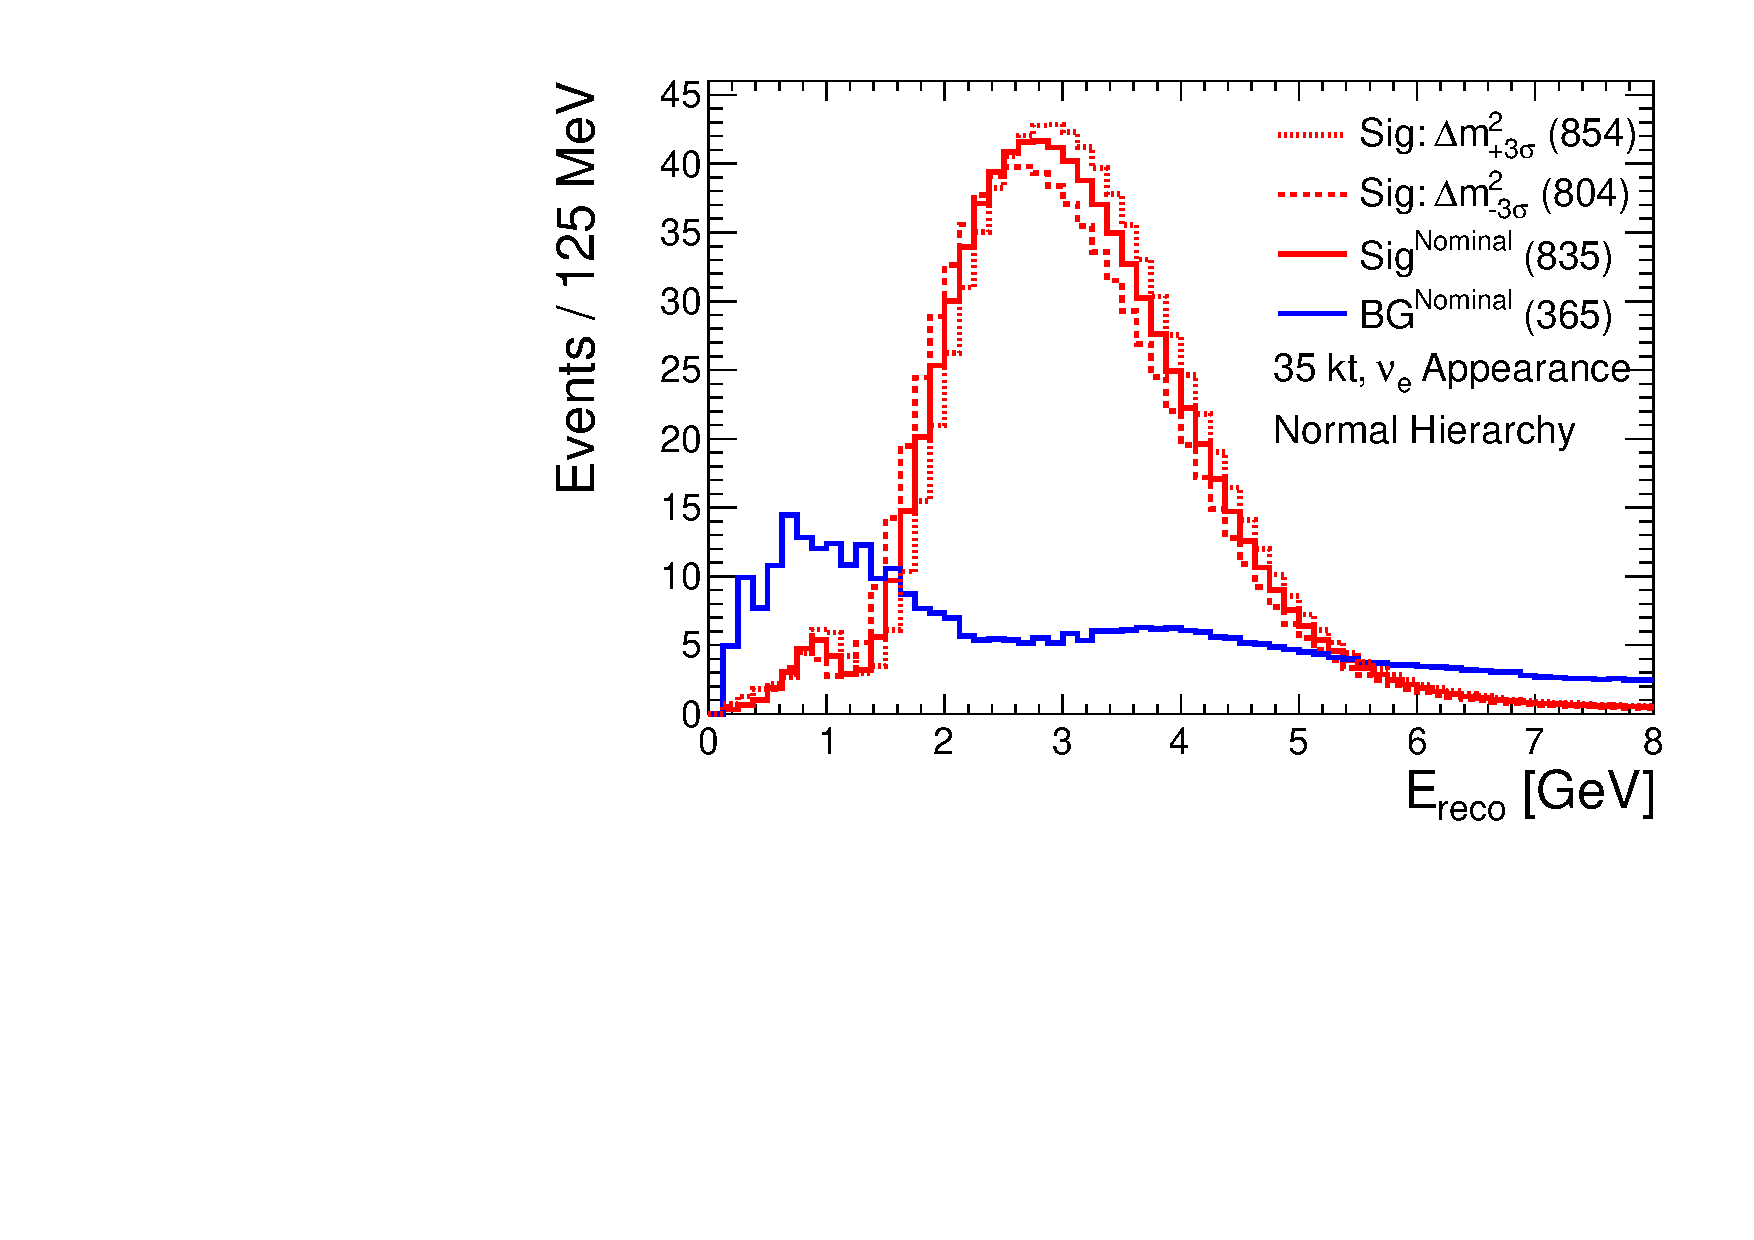
\includegraphics[width=0.45\textwidth]{figs/spectra_35kt_nue_dmvar_nh.pdf}
  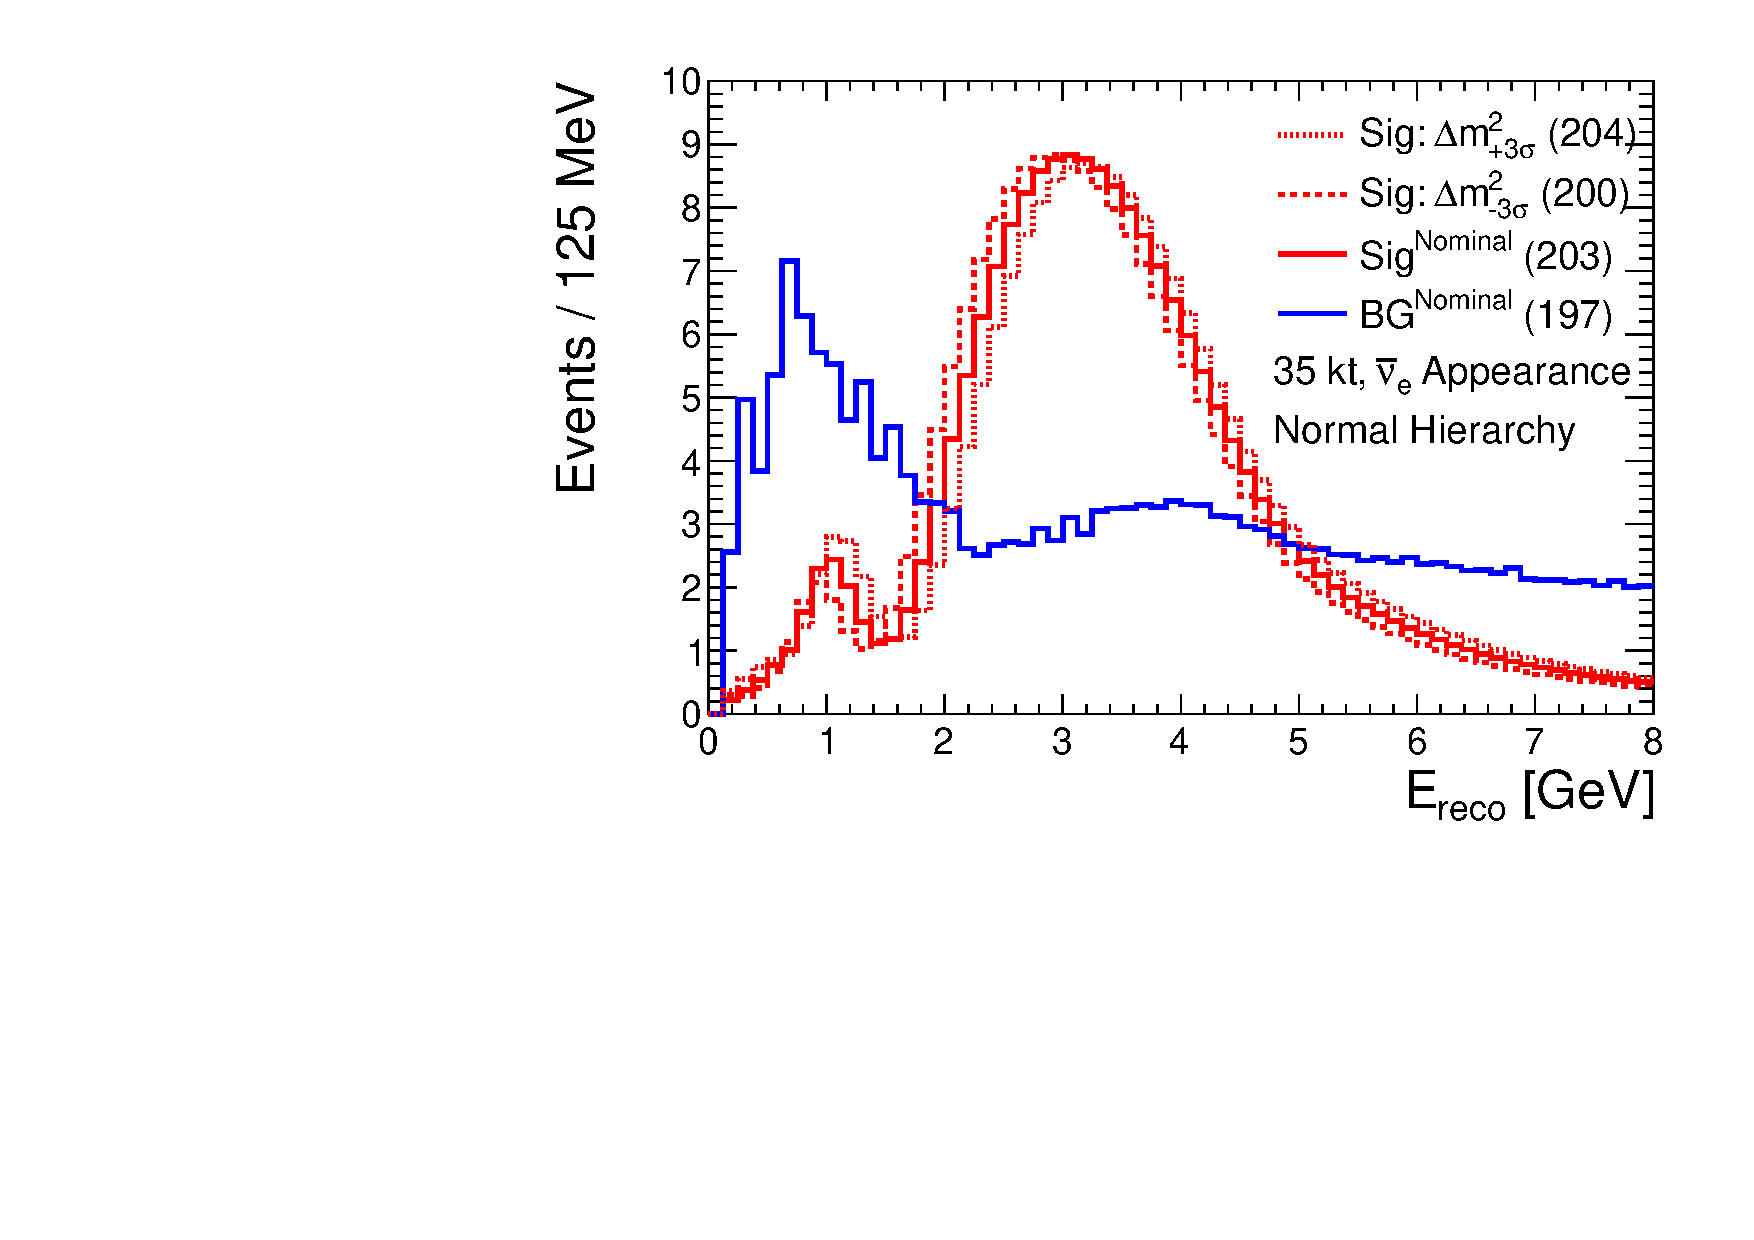
\includegraphics[width=0.45\textwidth]{figs/spectra_35kt_nuebar_dmvar_nh.pdf}
  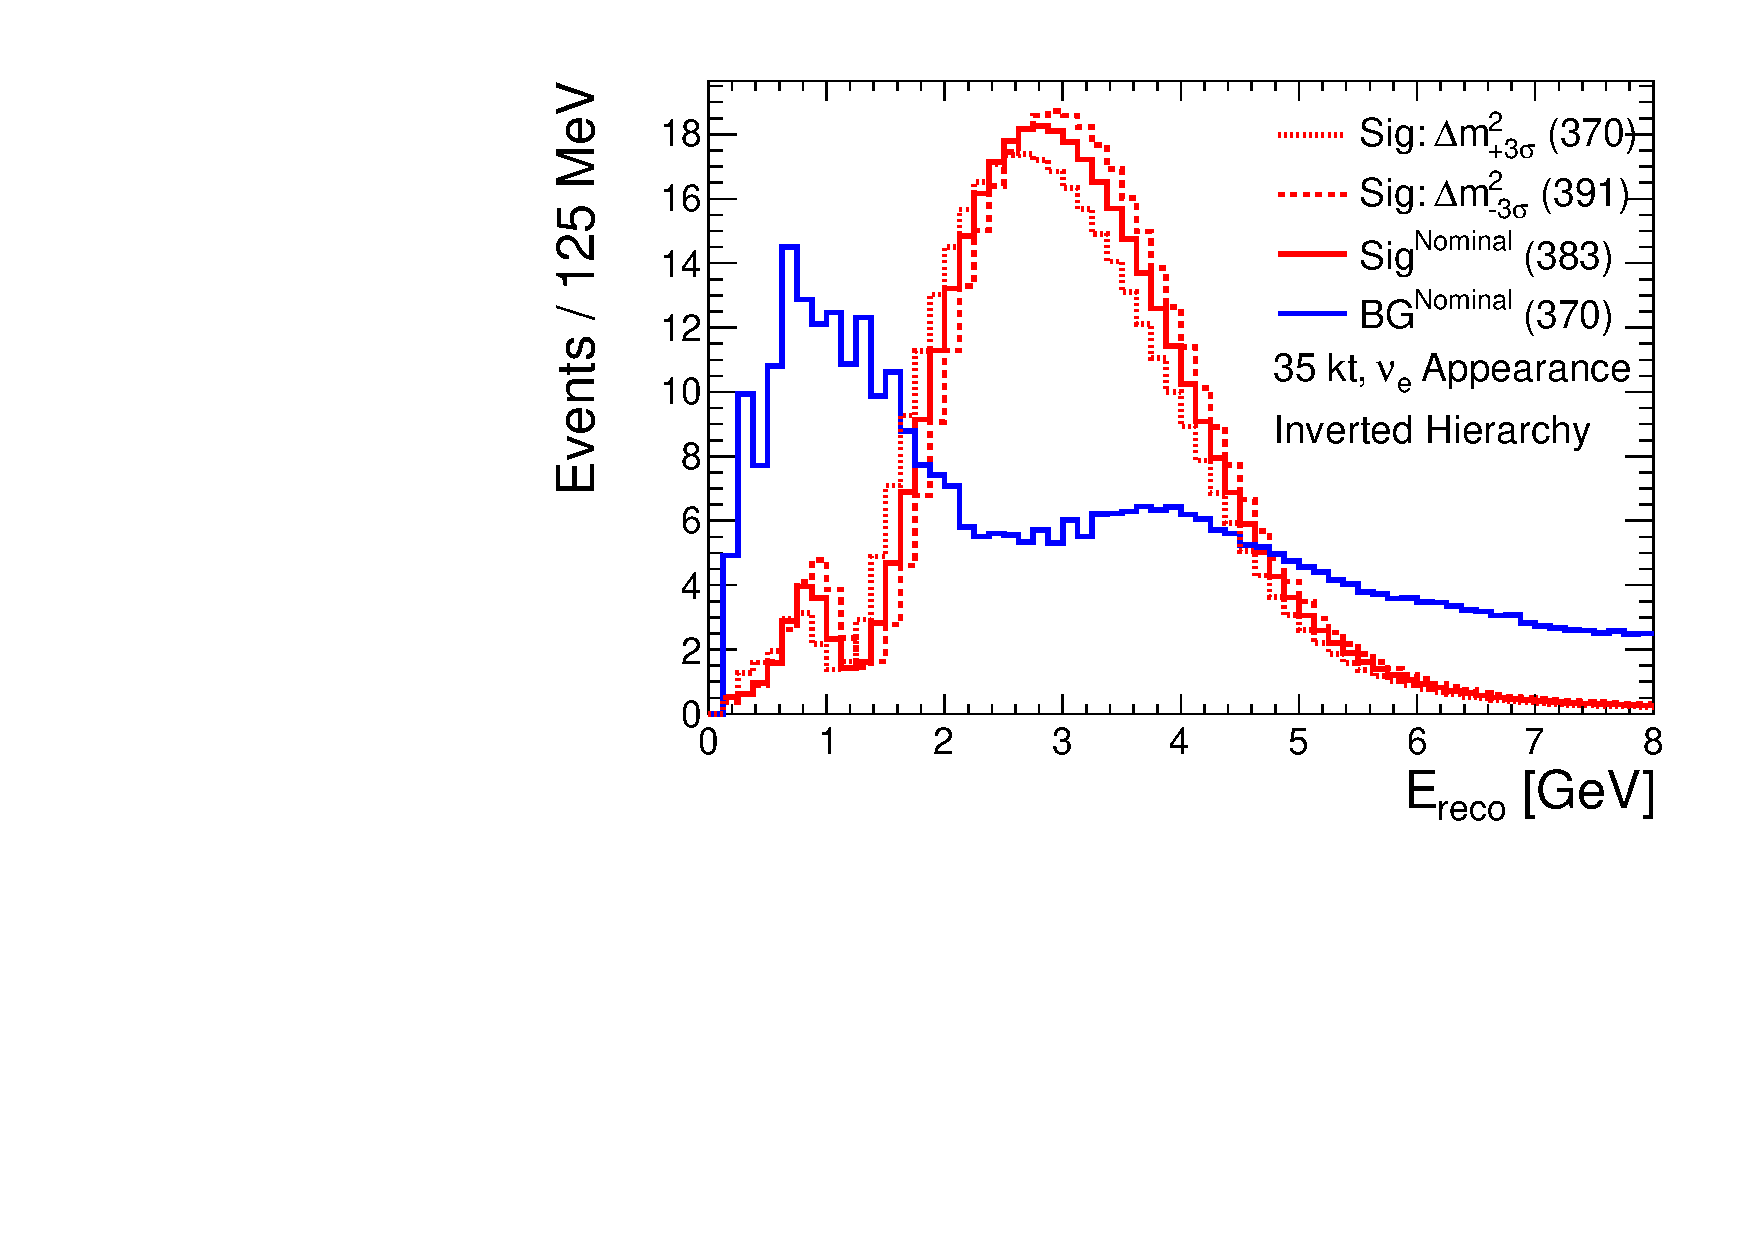
\includegraphics[width=0.45\textwidth]{figs/spectra_35kt_nue_dmvar_ih.pdf}
  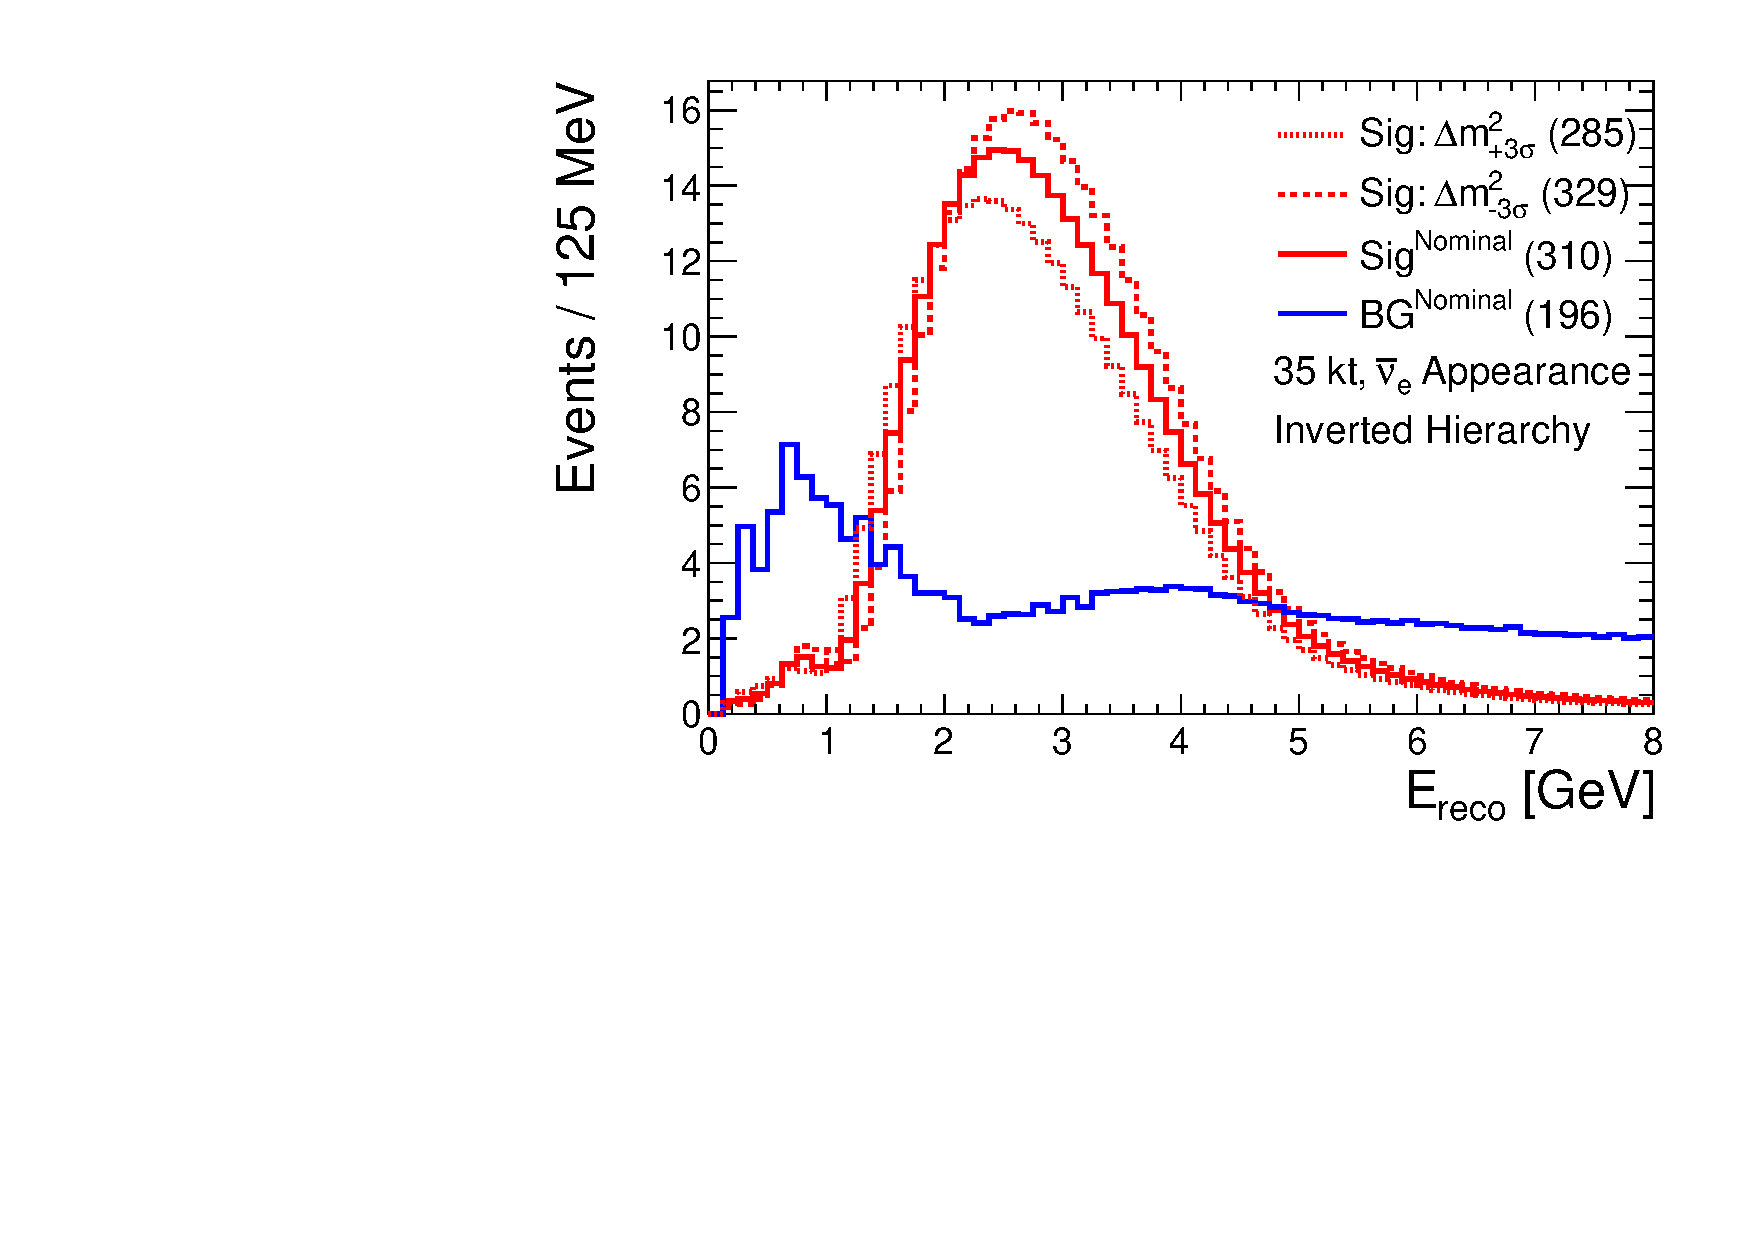
\includegraphics[width=0.45\textwidth]{figs/spectra_35kt_nuebar_dmvar_ih.pdf}
  \caption{
  Variations in $\delta m^2_{31}$:
  $\nu_e$~appearance (left) and $\overline{\nu}_e$~appearance (right) spectra 
  produced by GLoBES for a 35-kt LArTPC with 3 years of 
  exposure in an 80-GeV, 1.2-MW beam,  for true NH (top) and true IH (bottom). 
  The effect of varying the true
  value of $\Delta ,^2_{31}$ within its 3$\sigma$ allowed range is shown. 
  The total background, which does not depend on value of $\Delta m^2_{31}$ (CHECKME), 
  is overlaid on the signal. The total number
  of signal and background events are indicated in parenthesis.}
  \label{fig:dmspec}
\end{figure}
Figure~\ref{fig:dmsqsens} shows the variation in MH and CPV sensitivity when 
$\Delta m^2_{31}$
is varied within its 1$\sigma$ and 3$\sigma$ allowed range. In each case, the 
nominal relative constraints on all oscillation parameters, including $\Delta m^2_{31}$,
are applied and the normalization constraints are the nominal
1\% for signal and 5\% for background.
\begin{figure}[!htb]
  \centering
  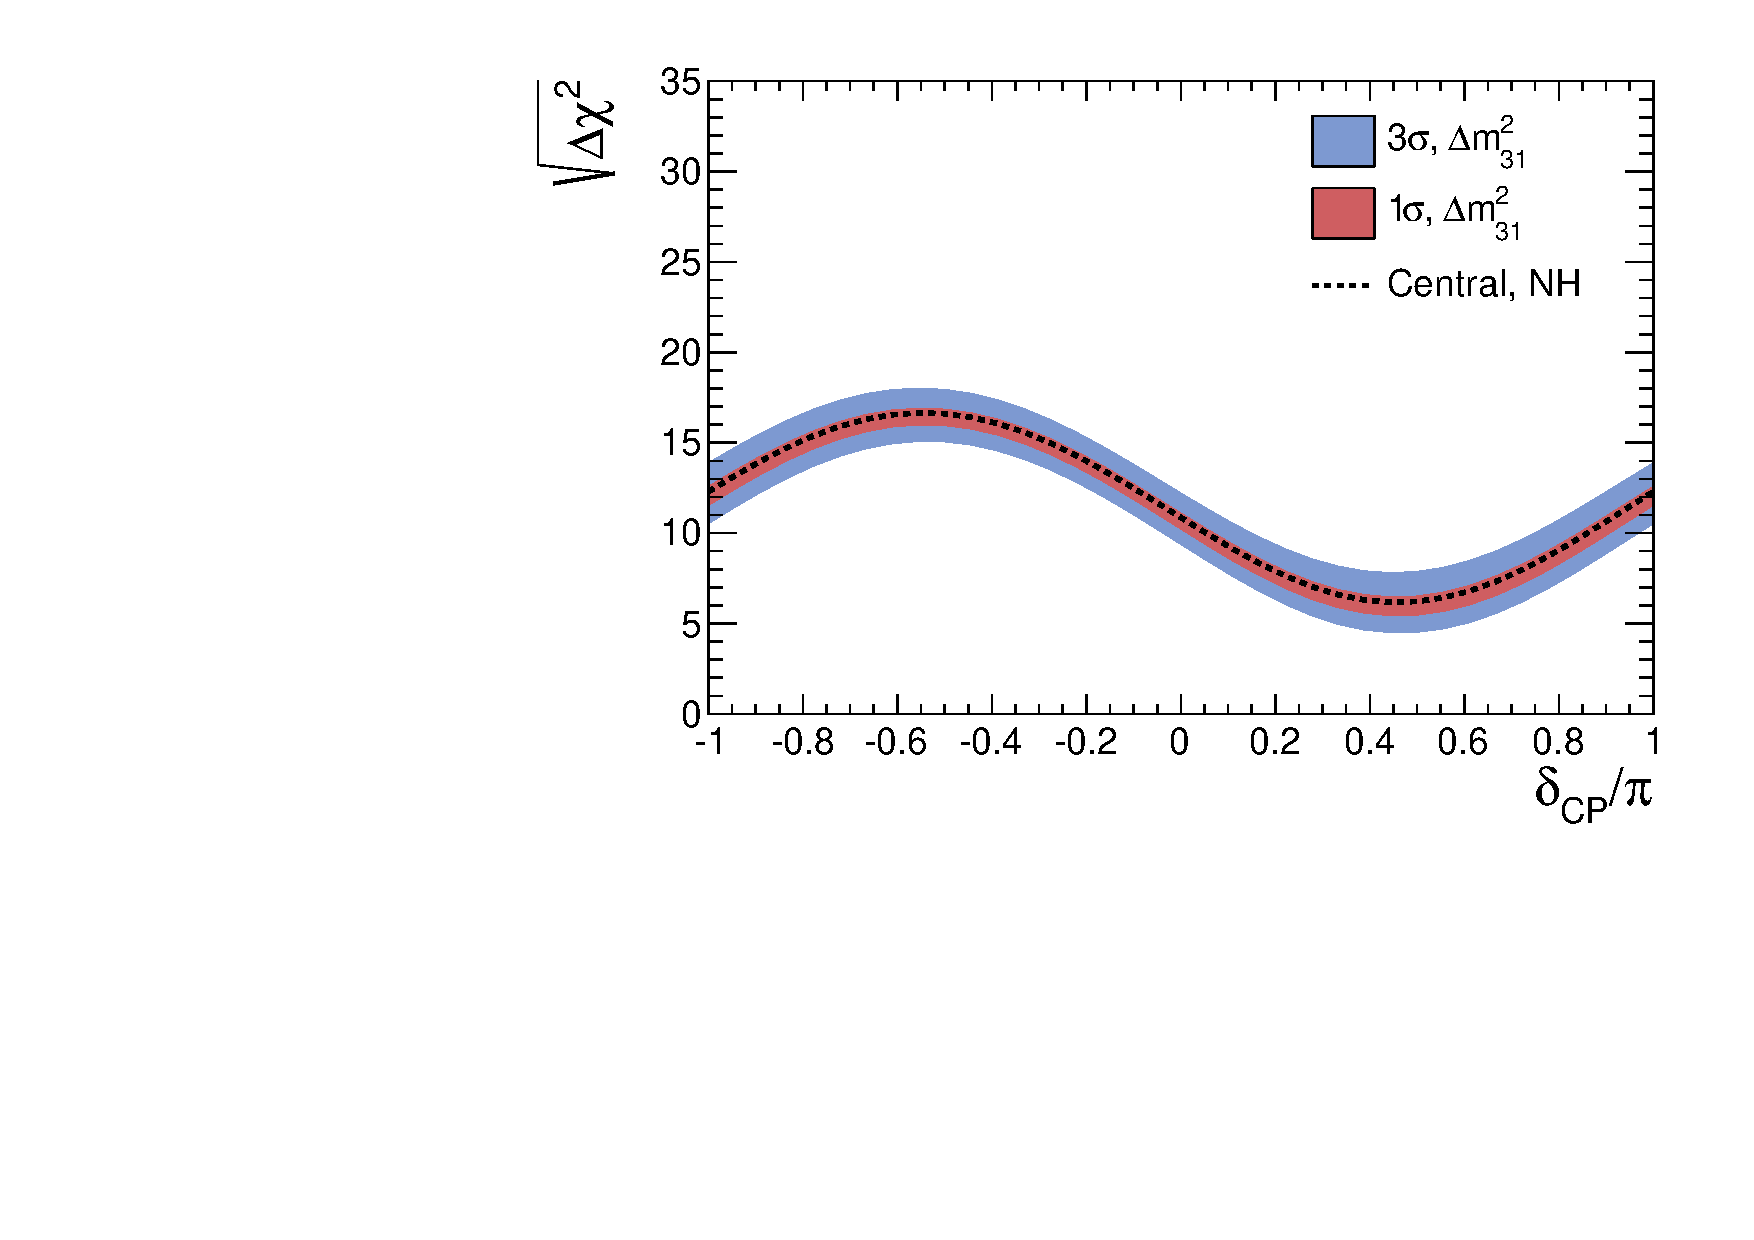
\includegraphics[width=0.45\textwidth]{figs/mh_35kt_nh_dmsq.pdf}
  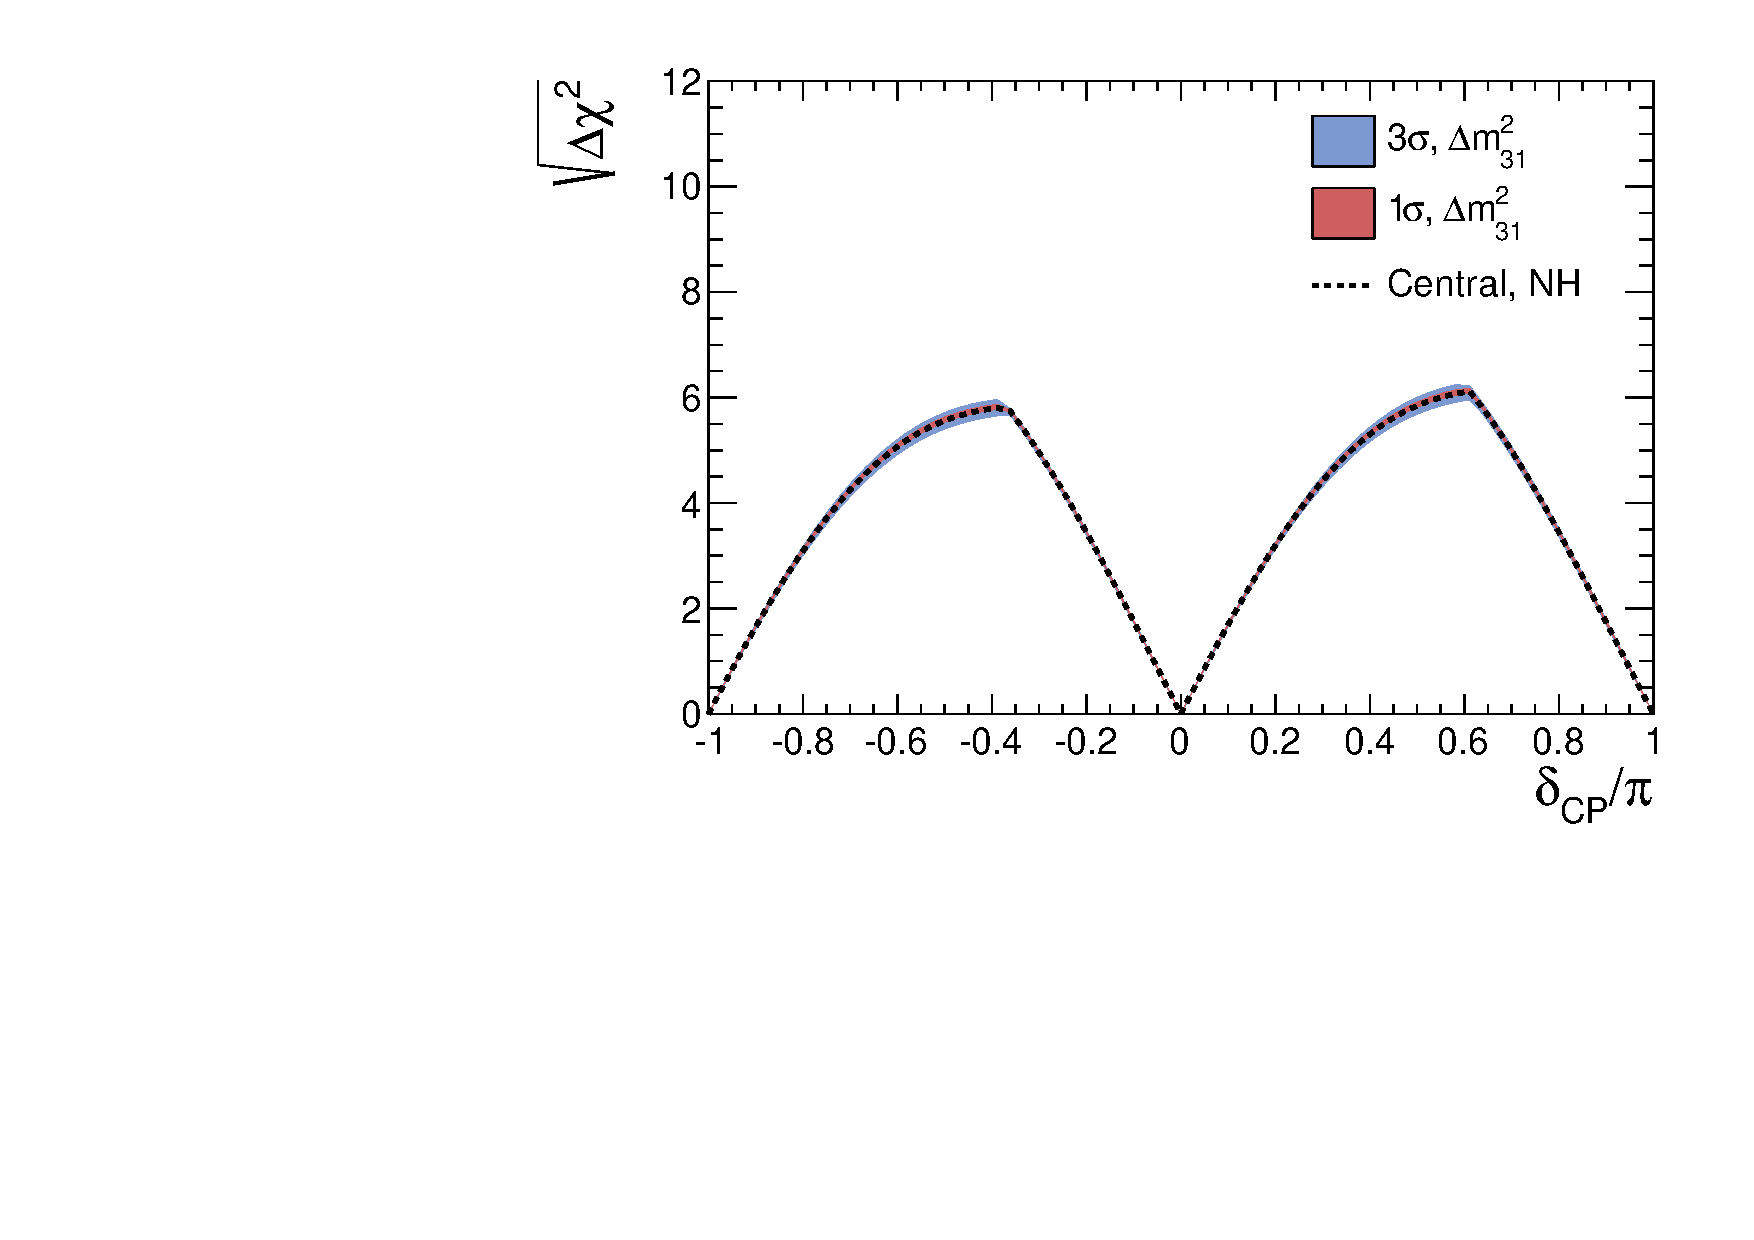
\includegraphics[width=0.45\textwidth]{figs/cpv_35kt_nh_dmsq.pdf}
  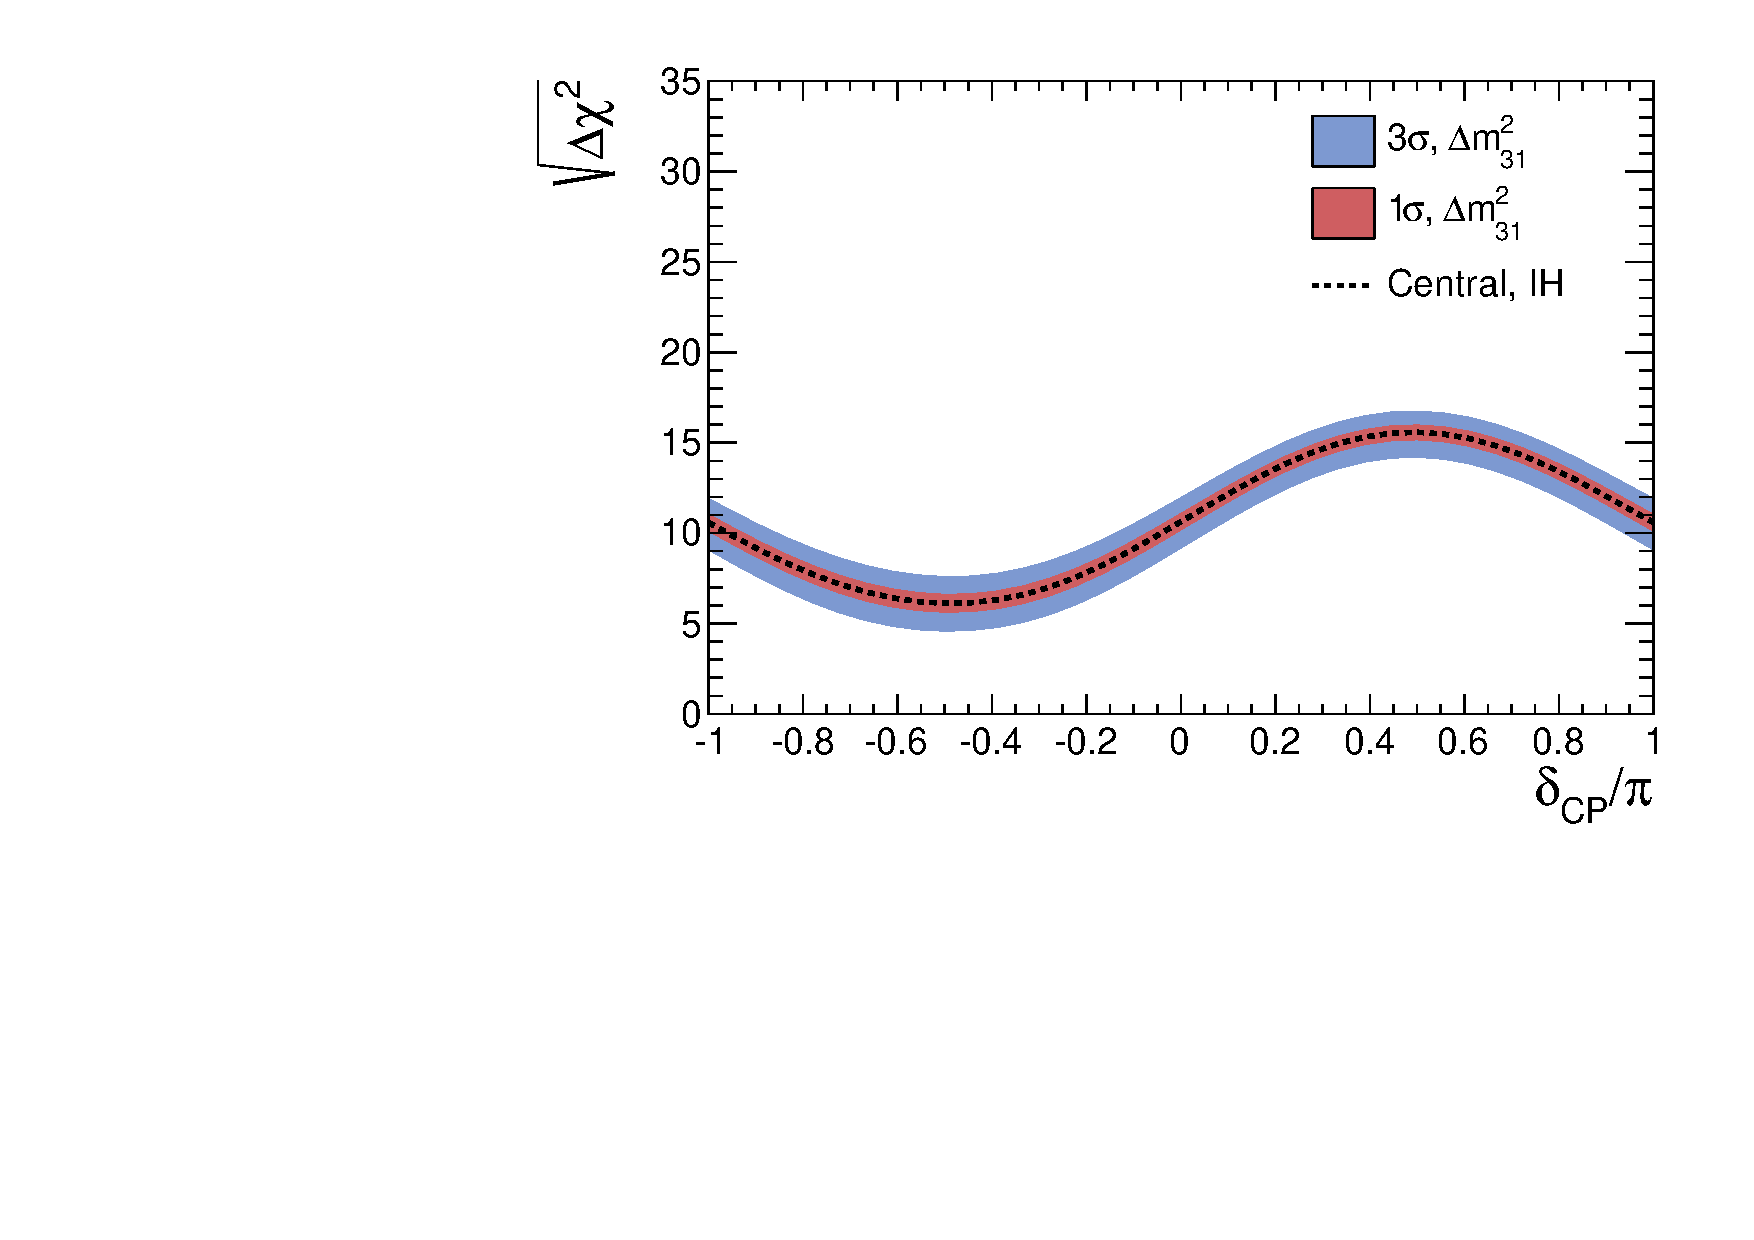
\includegraphics[width=0.45\textwidth]{figs/mh_35kt_ih_dmsq.pdf}
  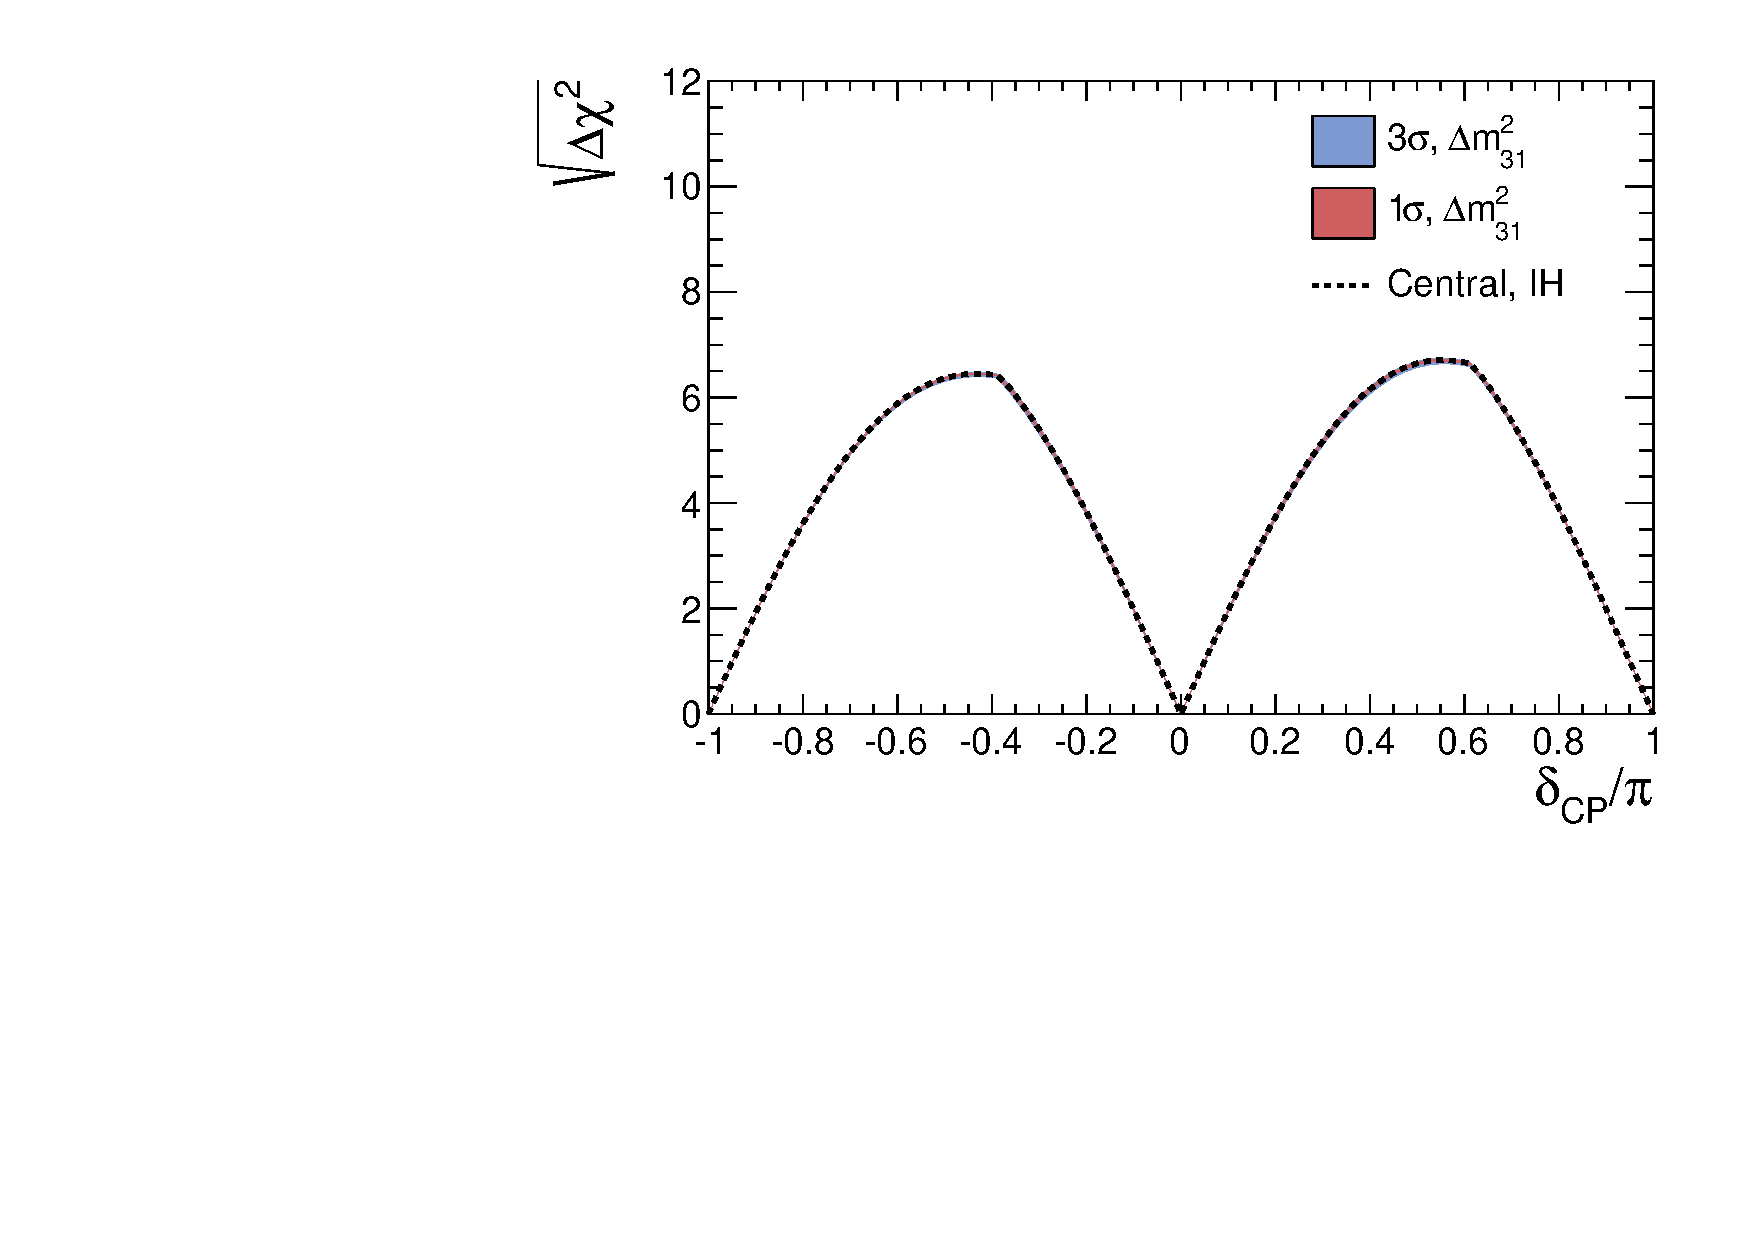
\includegraphics[width=0.45\textwidth]{figs/cpv_35kt_ih_dmsq.pdf}
  \caption{
  Variations in $\Delta m^2_{31}$: 
  MH (left) and CPV (right) sensitivities 
  produced by GLoBES for a 35-kt LArTPC with 3+3 ($\nu + \overline{\nu}$) years of 
  exposure in an 80-GeV, 1.2-MW beam,  for true NH (top) and true IH (bottom). 
  The effects of varying the true
  value of $\Delta m^2_{31}$ within its 1$\sigma$ (red band) and 3$\sigma$ (blue band)
  allowed ranges are shown.} 
  \label{fig:dmsqsens}
\end{figure}

\section{Sensitivity Dependence on $\delta_{CP}$}
\label{sect:deltacp}
The variation in $\nu_{\mu}$~disappearance, $\overline{\nu}_{\mu}$~disappearance, 
$\nu_e$~appearance, and $\overline{\nu}_e$~appearance with variations in the true
value of $\delta_{CP}$ is shown in Fig.~\ref{fig:example_spectra}.
\begin{figure}[!htb]
  \centering
  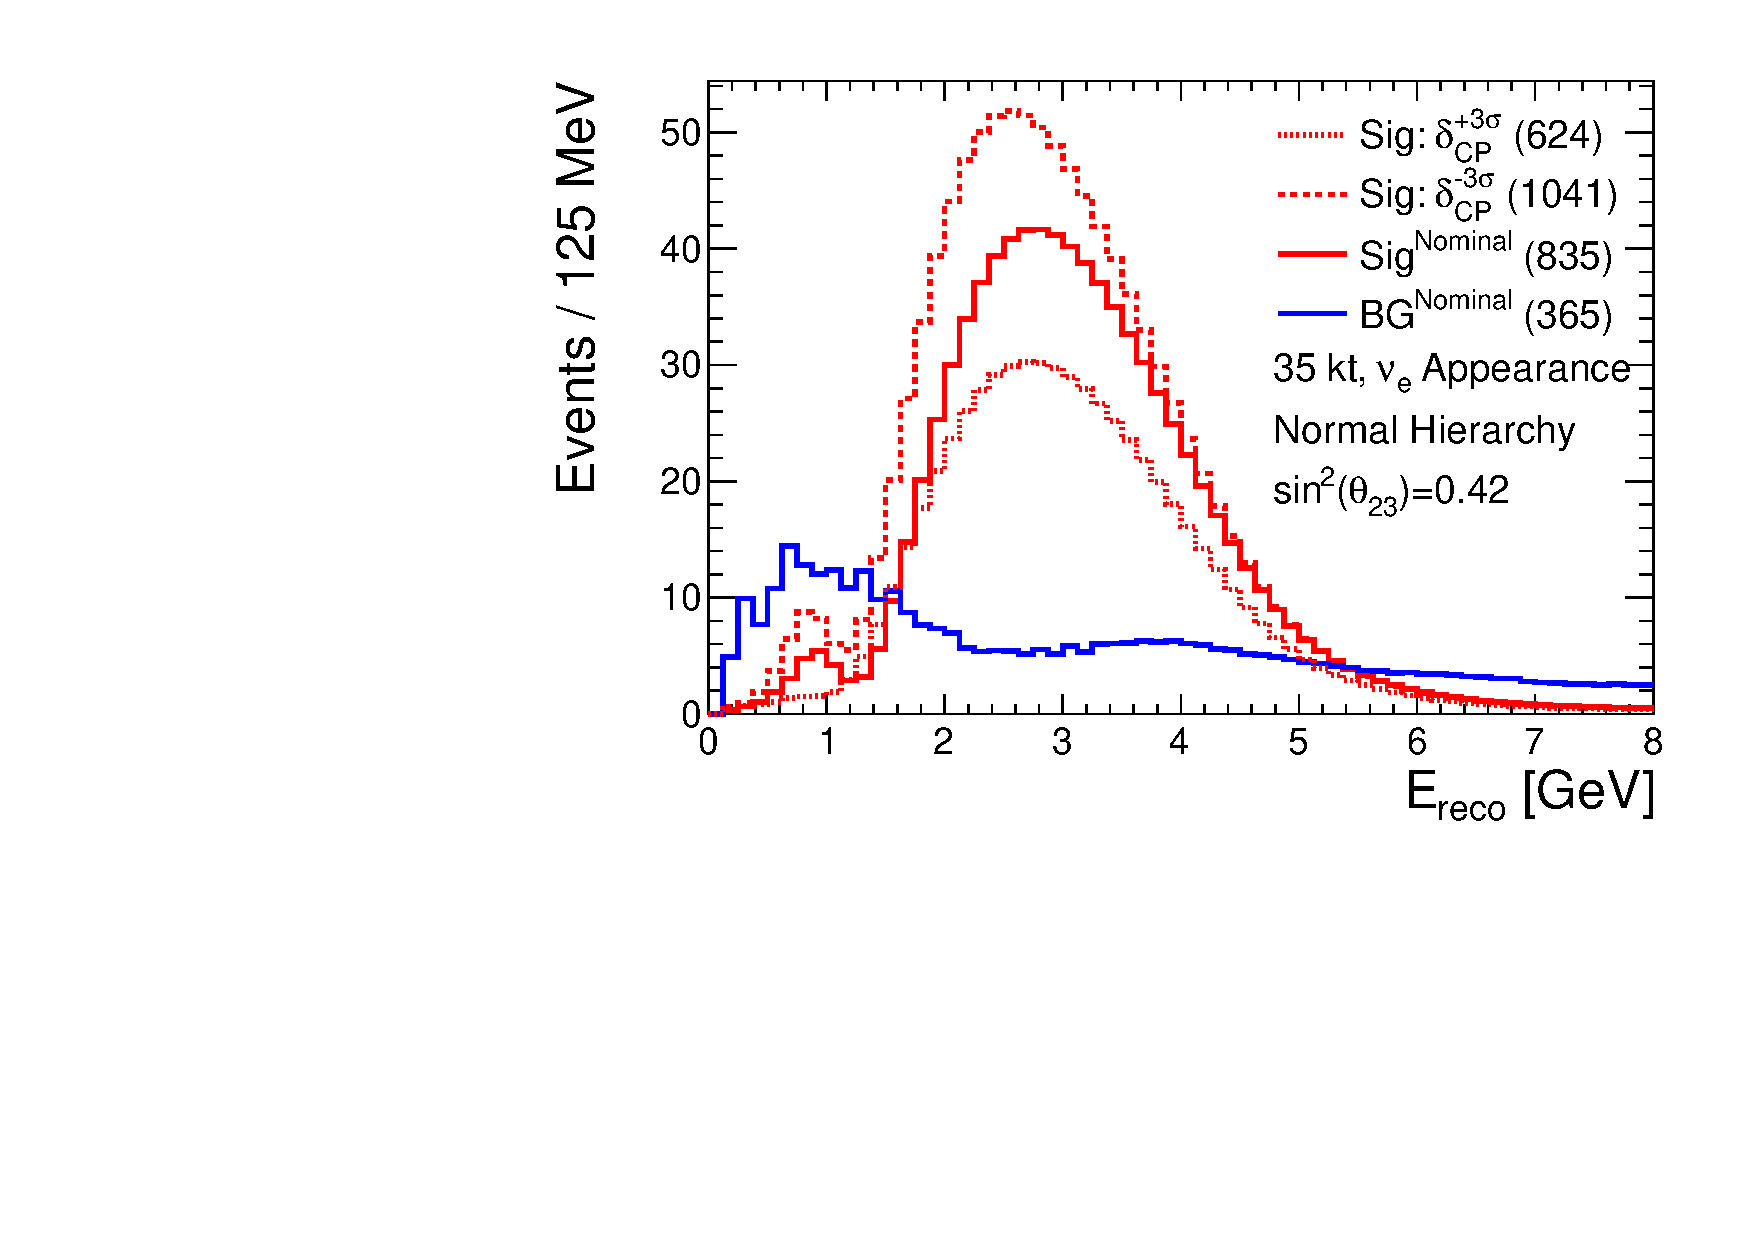
\includegraphics[width=0.45\textwidth]{figs/spectra_35kt_nue_dcpvar_nh.pdf}
  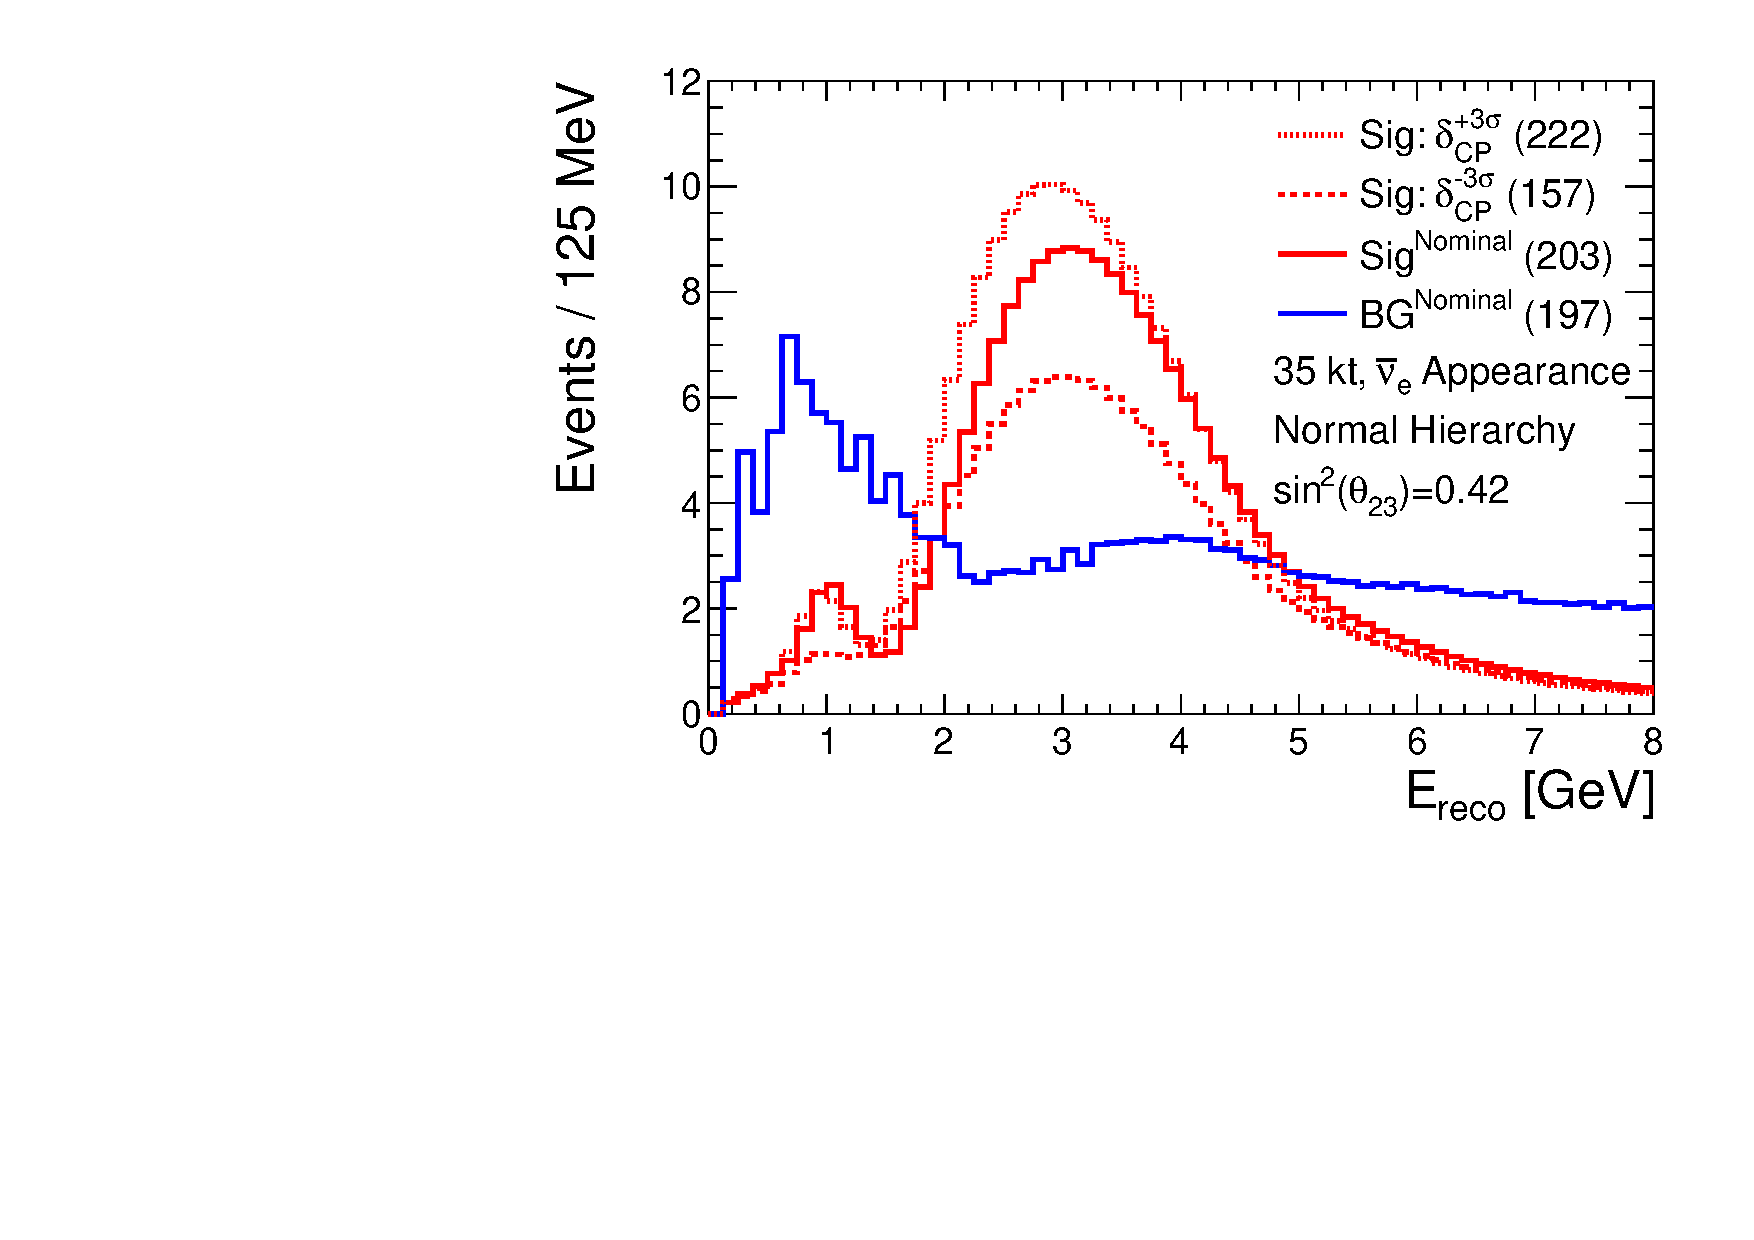
\includegraphics[width=0.45\textwidth]{figs/spectra_35kt_nuebar_dcpvar_nh.pdf}
  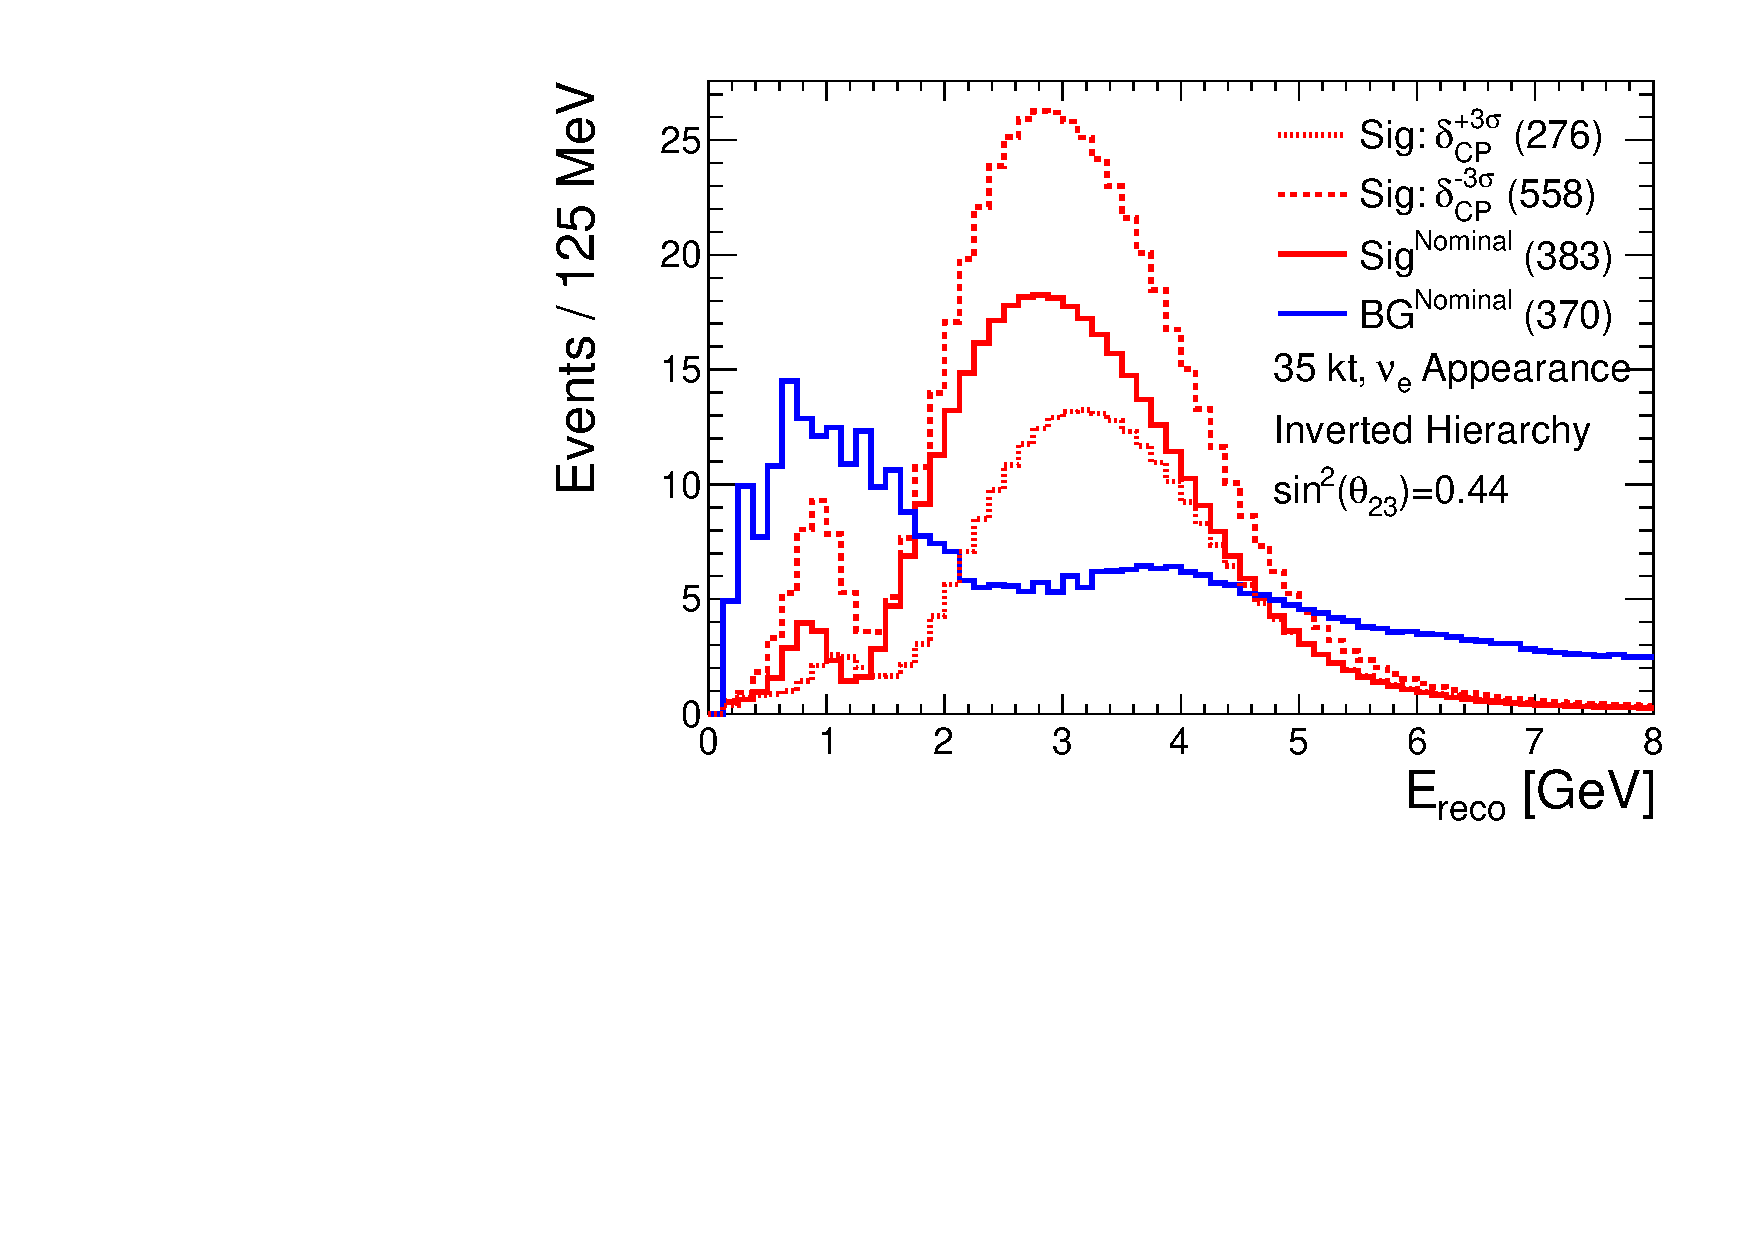
\includegraphics[width=0.45\textwidth]{figs/spectra_35kt_nue_dcpvar_ih.pdf}
  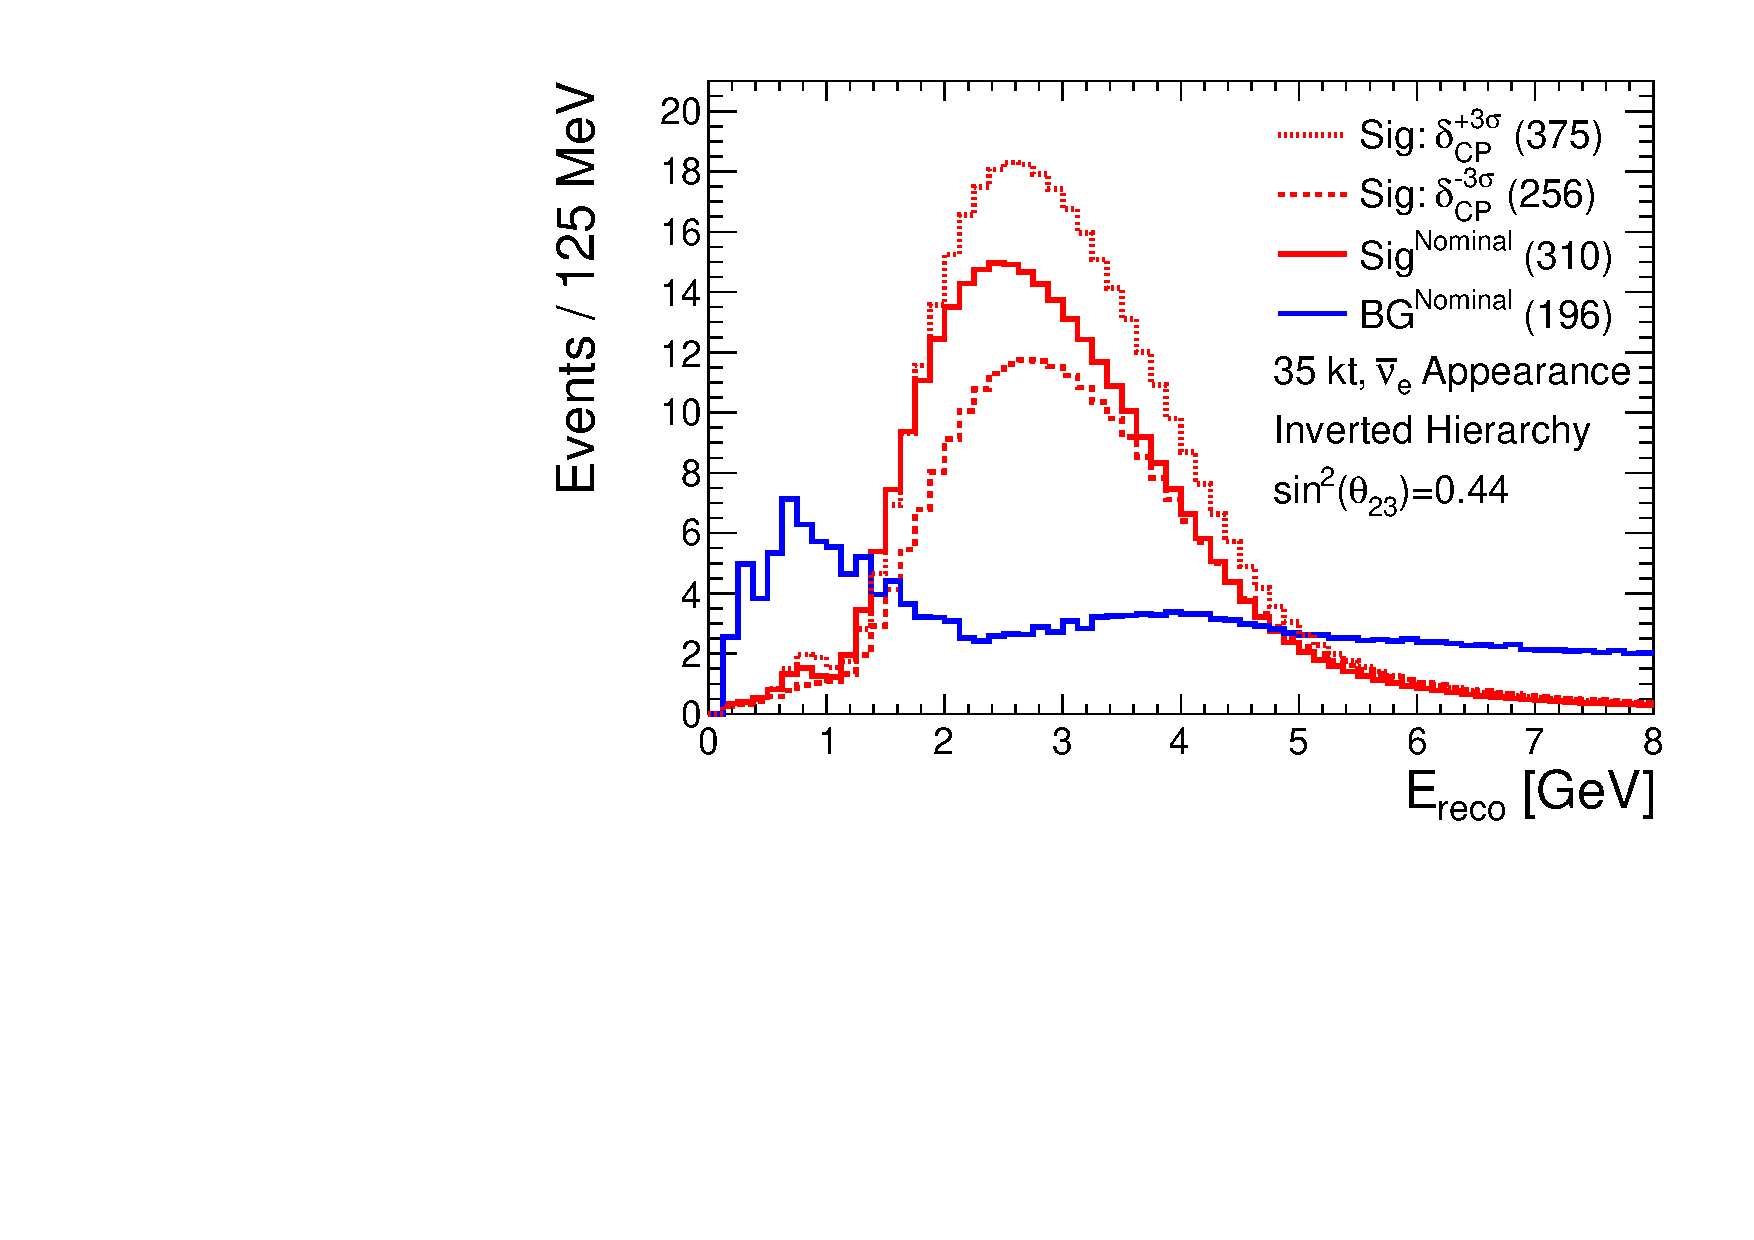
\includegraphics[width=0.45\textwidth]{figs/spectra_35kt_nuebar_dcpvar_ih.pdf}
  \caption{
  Variations in $\delta_{CP}$:
  $\nu_e$~appearance (left) and $\overline{\nu}_e$~appearance (right) spectra 
  produced by GLoBES for a 35-kt LArTPC with 3 years of 
  exposure in an 80-GeV, 1.2-MW beam, for true NH (top) and true IH (bottom). 
  The effect of varying the true
  value of $\delta_{CP}$ from $-\pi/2$ to zero to $\pi/2$ is shown.
  The total background, which does not depend on value of $\delta_{CP}$ (CHECKME), 
  is overlaid on the signal. The total number
  of signal and background events are indicated in parenthesis.}
  \label{fig:dcpspec}
\end{figure}

\section{Conclusions}
\label{sect:conclude}

\bibliography{refs}
\bibliographystyle{lbnepaper}

\end{document}




